\documentclass[
    msc,		% (*) msc, prepmsc, bsc, prepbsc - degree
    % prepbsc(msc) Preparation of BSc (MSc) dissertation
    % bsc(msc) BSc graduation report/ MSc dissertation
    en,			% (*) pt, en - languages 
    twoside,	% (*) twoside, oneside - single or double sided printing
    12pt,		% (*) 12pt, 11pt, 10pt - use font size
    a4paper,	% Paper size/format
    utf8,			% (*) utf8, latin1	- Text encoding: Linux, Mac or Windows
    onscreen, % (*) onscreen, onpaper - Page layout: screen versus paper print
    hyperref = true,  % (*) true, false - Hyperlinks in citations
    listof=totoc
]{thesisisel}

\usepackage{tabularx}
\usepackage[export]{adjustbox}

\lstdefinestyle{mystyle}{
    basicstyle=\ttfamily\footnotesize,
    frame=single,
    numbers=left,
}
\lstset{style=mystyle}

\addbibresource{references.bib}
\graphicspath{ {images/} }

\newacronym{nft}{NFTs}{Non-Fungible Tokens}
\newacronym{dapp}{DApps}{Decentralized Applications}
\newacronym{defi}{DeFi}{Decentralized Finance}
\newacronym{ecdsa}{ECDSA}{Elliptic Curve Digital Signature Algorithm}
\newacronym{rsa}{RSA}{Rivest-Shamir-Adleman}
\newacronym{pow}{PoW}{Proof of Work}
\newacronym{pos}{PoS}{Proof of Stake}
\newacronym{poh}{PoH}{Proof of History}
\newacronym{evm}{EVM}{Ethereum Virtual Machine}
\newacronym{ipfs}{IPFS}{InterPlanetary File System}
\newacronym{erc}{ERC}{Ethereum Request for Comment}
\newacronym{uml}{UML}{Unified Modeling Language}
\newacronym{uri}{URI}{Uniform Resource Identifier}

\def\thetitle{Ticket management system using Blockchain technology}
\def\theauthor{Rodrigo Filipe Leitão Dias}

%% Title of thesis
\title{ \thetitle }

%% Author(s) 
% gender: f for women or m for men and name
%  ------ Master report  (maximum of 1) ---------
\author[m]{\uppercase{\theauthor}}
\authordegree{(Licenciado)}

%  ------ Bachelor report  (maximum of 3) ---------
%\author[f]{\uppercase{[Nome completo do primeiro autor]}}
%\author[f]{\uppercase{[Nome completo do segundo autor]}}
%\author[f]{\uppercase{[Nome completo do terceiro autor]}}
%% remove text inside { } for report document
%\authordegree{} 

%% Date
\themonth{Setembro }
\theyear{2024}

%% Supervisors (maximum of 2)
% use [f] for female and [m] for male
%% ---------------------------------------------------%%
%% \adviser[m|f]{Category}{Name}
%% ---------------------------------------------------%%
\adviser[m]{Carlos Jorge de Sousa Gonçalves}{Doutor}

%
%% Jury (maximum of 5 elements)
%% Use [p] for president, of the jury and [a] for referees
%% ---------------------------------------------------%%
%% \jury[p|a]{Category and Name}
%% ---------------------------------------------------%%
\jury[p]{Doutor António Gelásio Frazão Isidro Teófilo}
%% Referees
\jury[a]{Doutor José Manuel de Campos Lages Garcia Simão}
\jury[a]{Doutor Carlos Jorge de Sousa Gonçalves}
% \jury[a]{[Grau e  Nome do segundo vogal]}
%\jury[a]{[Grau e  Nome do terceiro vogal]}
%\jury[a]{[Grau e  Nome do quarto vogal]}

\hypersetup{
    pdftitle={ \thetitle},
    pdfauthor={ \theauthor},
    pdfsubject={ },
    pdfkeywords={{ }, { }, { }}
}


\begin{document}

% \frontmatter
\printcoverpage

\chapter*{Abstract}

The traditional ticketing industry faces challenges such as ticket scalping,
fraud, and limited transparency in secondary markets. Blockchain technology has
the potential to revolutionize ticketing by offering a secure, transparent, and
efficient solution. This thesis proposes a blockchain-based ticketing system
that leverages the core strengths of blockchain technology to address these
shortcomings.

The system utilizes smart contracts to manage the ticket lifecycle securely,
from creation by event organizers to purchase and transfer by users. This
ensures authenticity and eliminates the risk of counterfeiting. Additionally,
the system facilitates a secure and transparent secondary market for ticket
resale, with fair pricing mechanisms and clear ownership tracking.

\paragraph{Keywords:} Blockchain, Ticketing System, NFTs

\chapter*{Resumo}

A indústria tradicional de bilhetes enfrenta desafios como a revenda ilegal de
bilhetes, fraude e transparência limitada nos mercados secundários. A
tecnologia blockchain tem o potencial de revolucionar o setor de bilheteiras ao
oferecer uma solução segura, transparente e eficiente. Esta tese propõe um
sistema de bilheteira baseado em blockchain que aproveita as principais
capacidades desta tecnologia para resolver esses problemas.

O sistema utiliza \textit[smart contracts] para gerir de forma segura o ciclo
de vida dos bilhetes, desde a criação pelos organizadores de eventos até à
compra e transferência pelos utilizadores. Isto garante a autenticidade e
elimina o risco de falsificação. Além disso, o sistema facilita um mercado
secundário seguro e transparente para a revenda de bilhetes, com mecanismos de
preços justos e um rastreio claro de propriedade.

\paragraph{Palavras-chave:} Blockchain, Sistema de Bilheteira, NFTs

\tableofcontents
\listoffigures
\listoftables
\lstlistoflistings
\printnoidxglossaries

\chapter{Introduction}
\label{ch:introduction}

Concerts and festivals play a big role in peoples life's, allowing them to
create memorable experiences watching live performances from their favorite
artists. Those are the kinds of memories that last for life, so every event
organizer wants to ensure that the whole process works seamlessly, from the end
user to the entire background planning of the event.

The process of organizing an event starts with the event organizer, who is
responsible for the whole planning of the event, from the venue to the artists,
to the marketing and ticketing. The event organizer is the one who takes the
risk of organizing the event, and the one who will profit from it, and can be a
company, a group of people, or even a single person, whom will hire the
artists, the venue, the security, the marketing, and the ticketing.

However, there's an issue with the ticketing process, which is the scalping.
Scalping is the process of buying tickets in bulk, exploiting high demand, and
reselling them at significantly inflated prices. This not only disadvantages
for people that genuinely want to attend but also undermines the integrity of
the ticketing system. Traditional ticketing platforms often rely on centralized
databases and intermediaries, providing opportunities for scalpers to
manipulate the system and engage in fraudulent activities. Moreover, existing
ticketing systems frequently encounter issues related to security, trust, and
reliability. Centralized databases are vulnerable to cyber attacks, leading to
unauthorized access, data breaches, and the manipulation of ticketing
information. Trust in the authenticity of tickets and the reliability of
transactions is compromised, creating a pressing need for innovative solutions
that can address these inherent challenges.

That's where blockchain comes in. Blockchain technology, renowned for its
decentralized and transparent nature, presents a compelling solution to
revolutionize the ticketing industry. By leveraging blockchain, it becomes
possible to create a secure and tamper-proof ledger of transactions, mitigating
the risk of scalping and ensuring the integrity of the ticketing process. The
use of smart contracts further automates transactions, reducing the reliance on
intermediaries, therefore extra costs, and enhancing operational efficiency.
This allows the event organizer to have a more secure and reliable ticketing
process, and the end user to have a more transparent and fair ticketing
process.

\section{Motivation}

The motivation for this work is primarily to avoid ticket scalping. This is the process of buying tickets in bulk, exploiting high demand, and reselling them at significantly inflated prices. This not only disadvantages people that genuinely want to attend but also undermines the integrity of the ticketing system. Traditional ticketing platforms often rely on centralized databases and intermediaries, providing opportunities for scalpers to manipulate the system and engage in fraudulent activities. By using blockchain, it's possible to create a system that prevents any kind of unwanted operations, because of the properties of smart contracts, that enforce a certain behavior, allowing for users to resell a ticket, but not for a price higher than the original price. This is a way to guarantee that the end user will have a fair and transparent ticketing process.

For this to happen, the idea is to have a marketplace for users to resell their tickets, enforcing a price cap. With this feature, it's also possible to have a way for the organizer to promote the event on this platform, giving the possibility of reducing costs, by removing intermediaries like marketing companies.

Another important feature is the possibility of having partial refunds. This is something that is not always available in traditional ticketing platforms, and when it is, it's not always easy to do. With blockchain, it's possible to have a system that allows for easy and instant refunds, without the need for intermediaries. Enabling a feature like this can actually be advantageous for the organizers, if they're expecting the venue to be full. This way, when users buy their tickets and then realize they can't attend, they have a reason to refund, making that ticket available again for the original price, making a profit for the organizer.

Another point, and the main reason to use blockchain, is to guarantee the user of any operation. In the traditional ticketing system, there can be human errors, or even fraud, and this assures users that any operation defined will never change and will be executed as expected.
\section{Objectives}

{\color{red}
\begin{itemize}
    \item develop smart contracts
    \item app for users to manage their tickets
    \item authentication logic on tickets to verify ticket ownership
    \item develop dashboard to allow event organizers to deploy their events
\end{itemize}
}

\section{Contributions}

 [website]
 [user app]
 [validator app]
\section{Document Structure}
\label{sec:document_structure}

The document is structured in the following way: \textbf{Chapter
    ~\ref{ch:introduction}: Introduction} provides an overview of the project,
including its context, motivation, objectives, and contributions;
\textbf{Chapter~\ref{ch:background_and_related_work}: Background and Related
    Work} introduces essential concepts and technologies that serve as the
foundation for the project; \textbf{Chapter~\ref{ch:requirements_analysis}:
    Requirements Analysis} outlines the functional and non-functional requirements
of the project as well as the use cases and the architecture; \textbf{Chapter
    ~\ref{ch:implementation}: Implementation} describes the implementation of the
project, including the technologies used; \textbf{Chapter~\ref{ch:results}:
    Results} presents the results of the project and how it meets the requirements;
\textbf{Chapter~\ref{ch:conclusions}: Conclusions} summarizes the project,
reflecting on the achievements and limitations, and suggesting future work.


\pagebreak
\chapter{Background and Related Work}
\label{ch:background_and_related_work}

[Brief introduction of the chapter]

\section{Background}

\subsection{Blockchain}

Blockchain is a decentralized and distributed ledger technology that enables the secure recording and sharing of data across a network of computers. At its core, a blockchain consists of a series of blocks, each containing a list of transactions. These blocks are linked together in a chronological and immutable chain, forming a transparent and tamper-proof record of transactions.

~

Key characteristics of blockchain technology include:
\begin{itemize}
    \item \textbf{Decentralization}: Unlike traditional centralized systems where data is stored in a single location or controlled by a central authority, blockchain operates on a decentralized network of computers (nodes). Each node maintains a copy of the entire blockchain, ensuring that there is no single point of failure or control.
    \item \textbf{Transparency}: The data recorded on a blockchain is visible to all participants in the network. This transparency fosters trust among users, as they can independently verify the integrity of transactions and the state of the ledger without relying on intermediaries.
    \item \textbf{Immutability}: Once a transaction is recorded on the blockchain and added to a block, it becomes virtually impossible to alter or delete. This immutability is achieved through cryptographic techniques such as hashing and consensus mechanisms, ensuring that the historical record of transactions remains tamper-proof.
    \item \textbf{Security}: Blockchain technology employs advanced cryptographic algorithms to secure transactions and protect the integrity of the network. Transactions are verified and validated by network participants through a process known as consensus, which prevents fraudulent or unauthorized changes to the ledger.
    \item \textbf{Smart Contracts}: Smart contracts are self-executing contracts with predefined rules and conditions written in code. These contracts automate the execution of transactions and enforce agreements without the need for intermediaries. Smart contracts enable the creation of decentralized applications (DApps) that run on blockchain networks, facilitating a wide range of use cases beyond simple monetary transactions.
\end{itemize}

Blockchain technology has applications across various industries, including finance, supply chain management, healthcare, and decentralized finance (DeFi). Its potential to revolutionize existing systems by enhancing security, transparency, and efficiency has led to widespread adoption and exploration of its capabilities in solving complex challenges. Some people refer to this ecosystem as Web3, which is a new paradigm for the internet that aims to decentralize control and empower users with greater ownership and privacy over their data and digital assets.
The reason a system like this works is because it leverages the human nature of greed and self-interest to create a system that is secure and reliable. The network of nodes is incentivized to maintain the integrity of the blockchain by rewarding them with cryptocurrency for their efforts. This creates a system where the majority of the network is honest and works together to maintain the integrity of the blockchain, making it resistant to attacks and fraud, as the cost of attacking the network would far outweigh any potential gains.

\subsection{Wallets}
Cryptocurrency wallets rely on cryptographic principles to securely manage and interact with digital assets on blockchain networks. These cryptographic techniques ensure the security and integrity of transactions while protecting the private keys that control access to cryptocurrency holdings.

~

Some of the key cryptographic aspects of wallets are:
\begin{itemize}
    \item \textbf{Private and Public Keys}: Cryptocurrency wallets utilize a pair of cryptographic keys: a public key and a private key. The public key, also known as the wallet address, is used to receive funds and is shared publicly. The private key, on the other hand, is known only to the wallet owner and is used to sign transactions and authorize the spending of funds. The relationship between the public key and the private key is based on asymmetric cryptography, where data encrypted with one key can only be decrypted with the other key. This ensures that transactions are secure and that only the rightful owner of the private key can access and control their cryptocurrency holdings.
    \item \textbf{Digital Signatures}: When a transaction is initiated from a cryptocurrency wallet, it is digitally signed using the wallet's private key. This digital signature serves as proof of authorization and ensures that the transaction cannot be tampered with or altered. Digital signatures are generated using cryptographic algorithms such as the Elliptic Curve Digital Signature Algorithm (ECDSA) or the Rivest-Shamir-Adleman (RSA) algorithm, depending on the specific blockchain network and protocol.
    \item \textbf{Hash Functions}: Cryptocurrency wallets use cryptographic hash functions to create a unique representation of transaction data, known as a transaction hash. These hash functions generate fixed-length strings of characters from input data, making it computationally infeasible to reverse-engineer the original data from the hash. Transaction hashes are essential for verifying the integrity of transactions and ensuring that they have not been altered or tampered with during transmission.
    \item \textbf{Seed Phrases and Mnemonic Codes}: Some cryptocurrency wallets use mnemonic codes or seed phrases as a backup mechanism for restoring access to wallet funds in case the original private key is lost or compromised. These seed phrases are generated from a random sequence of words and serve as a human-readable representation of the wallet's private key. They can be used to regenerate the private key and restore access to funds on a new wallet instance.
\end{itemize}

By leveraging these cryptographic techniques, cryptocurrency wallets provide a secure and reliable means for users to store, manage, and transact with digital assets on blockchain networks. The robustness of these cryptographic mechanisms ensures the confidentiality, integrity, and authenticity of transactions, safeguarding the value of cryptocurrency holdings against unauthorized access and fraudulent activities.

\subsection{Interacting with the Blockchain}

todo [explain what's needed to interact with the blockchain, with images]

~

As we saw, a blochchain works as a decentralized network of nodes, where each node has a copy of the entire blockchain. This means that in order to interact with the blockchain, we need to send transactions to the network, which will then be validated and added to a block by the nodes. To do this, we need to use a wallet, which is a software application that allows users to manage their digital assets, interact with smart contracts, and send transactions on the blockchain.
Wallets provide a user-friendly interface for accessing the blockchain network, signing transactions with private keys, and viewing account balances and transaction history. To execute a transaction on the blockchain, we need to sign it with our private key, which proves that we are the rightful owner of the assets being transferred. The transaction is then broadcast to the network, where it is validated by network participants and added to a block. Once the transaction is confirmed and included in a block, it becomes part of the immutable blockchain ledger, visible to all participants in the network.



\subsection{Networks}

This technology has evolved significantly since the inception of Bitcoin in 2009. Numerous platforms have emerged, each offering unique features, capabilities, and use cases.

~

Some of the most prominent networks that have gained traction in the decentralized ecosystem are:
\begin{itemize}
    \item \textbf{Bitcoin (BTC)}: Bitcoin is the first and most well-known cryptocurrency, introduced by an anonymous person or group of people under the pseudonym Satoshi Nakamoto in 2008. It operates on a decentralized network using a Proof of Work (PoW) consensus mechanism to validate transactions and secure the network. Bitcoin is designed as a peer-to-peer electronic cash system, enabling users to send and receive payments without the need for intermediaries. It has gained widespread adoption as a store of value and digital currency, with a fixed supply of 21 million coins and a deflationary monetary policy.
    \item \textbf{Ethereum (ETH)}: Ethereum is a decentralized, open-source blockchain platform that enables the creation and execution of smart contracts and decentralized applications (DApps). It introduced the concept of smart contracts, allowing developers to build a wide range of decentralized applications, from decentralized finance (DeFi) protocols to non-fungible token (NFT) marketplaces. Ethereum operates on a Proof of Work (PoW) consensus mechanism but is transitioning to a Proof of Stake (PoS) consensus model with the Ethereum 2.0 upgrade to improve scalability and energy efficiency.
    \item \textbf{Polygon (MATIC)}: Polygon is a Layer 2 scaling solution for Ethereum, designed to address the network's scalability issues by offering faster and cheaper transactions. It provides a framework for building and connecting Ethereum-compatible blockchain networks, known as sidechains, which leverage the security of the Ethereum mainnet. Polygon aims to enhance Ethereum's capabilities and support the mass adoption of
    \item \textbf{Solana (SOL)}: Solana is a high-performance blockchain platform designed for decentralized applications and crypto-currencies. It uses a unique combination of Proof of History (PoH) and Proof of Stake (PoS) consensus mechanisms to achieve high throughput and low latency, enabling fast transaction speeds and low fees. Solana aims to provide a scalable infrastructure for decentralized finance (DeFi), decentralized exchanges (DEXs), and other high-performance applications.
\end{itemize}

These are just a few examples of the diverse range of blockchain networks that exist, each offering unique features, capabilities, and use cases. As the blockchain ecosystem continues to evolve, new networks and technologies are constantly being developed, driving innovation and expanding the possibilities of decentralized applications and digital assets.

\subsection{Smart Contracts}
Smart contracts are self-executing contracts with the terms of the agreement directly written in code. These contracts automatically execute and enforce themselves when predefined conditions are met, without the need for intermediaries such as lawyers or notaries. Smart contracts run on blockchain platforms and are stored and executed across a decentralized network of nodes.

~

Key characteristics of smart contracts include:
\begin{itemize}
    \item \textbf{Autonomy}: Once deployed on the blockchain, smart contracts operate autonomously, executing transactions and enforcing agreements without human intervention. This autonomy ensures that contract terms are upheld impartially and transparently.
    \item \textbf{Trust}: Smart contracts leverage the trustless nature of blockchain technology, meaning that parties can trust the execution of the contract without relying on a trusted third party. The decentralized and immutable nature of blockchain ensures that contract terms are tamper-proof and transparent.
    \item \textbf{Security}: Smart contracts are highly secure due to the cryptographic principles underlying blockchain technology. Once deployed, smart contracts cannot be altered or tampered with, providing a high level of security and reliability.
    \item \textbf{Efficiency}: By automating contract execution, smart contracts eliminate the need for intermediaries, reducing costs and processing times associated with traditional contract enforcement. Transactions are executed quickly and efficiently, enhancing the overall speed and efficiency of business processes.
    \item \textbf{Versatility}: Smart contracts can be programmed to execute a wide range of functions beyond simple transaction processing. They can facilitate complex conditional agreements, manage digital assets, and even interact with other smart contracts, enabling the development of decentralized applications (DApps) with diverse functionalities.
\end{itemize}

Smart contracts have numerous applications across various industries, including finance, supply chain management, real estate, healthcare, and more. They are particularly well-suited for scenarios where trust, transparency, and automation are paramount, offering a revolutionary approach to contract execution and enforcement in the digital age.

\subsection{Token Standards}
Token standards play a crucial role in defining the rules and functionalities of digital tokens on blockchain networks. These standards provide a common framework that facilitates interoperability, compatibility, and ease of use for developers and users alike.

~

[add image]

~

Some of the most widely recognized token standards in the blockchain ecosystem are:
\begin{itemize}
    \item \textbf{ERC-20 (Ethereum Request for Comment 20)}: ERC-20 is the most commonly used token standard on the Ethereum blockchain, governing the creation and implementation of fungible tokens. These tokens are interchangeable and have identical properties, allowing them to be traded on cryptocurrency exchanges seamlessly. ERC-20 tokens adhere to a set of standard functions, including methods for transferring tokens, querying token balances, and approving token transfers on behalf of other addresses. Many of the initial coin offerings (ICOs), token sales, and decentralized finance (DeFi) projects on Ethereum utilize ERC-20 tokens due to their widespread adoption and compatibility with Ethereum wallets and exchanges.
    \item \textbf{ERC-721 (Ethereum Request for Comment 721)}: ERC-721 is a token standard on the Ethereum blockchain that governs the creation and implementation of non-fungible tokens (NFTs). Unlike ERC-20 tokens, each ERC-721 token is unique and indivisible, representing ownership or proof of authenticity of a specific asset. ERC-721 tokens are commonly used to represent digital assets such as digital art, collectibles, virtual real estate, and in-game items. Each token is assigned a unique identifier (token ID), allowing it to be distinguished from other tokens within the same contract. The ERC-721 standard defines methods for transferring tokens, querying token ownership, and managing metadata associated with each token, enabling a wide range of use cases in the burgeoning NFT market.
    \item \textbf{ERC-1155 (Ethereum Request for Comment 1155)}: ERC-1155 is a token standard on the Ethereum blockchain that supports the creation and management of both fungible and non-fungible tokens within the same contract. This allows developers to efficiently manage multiple token types and reduce gas costs associated with deploying multiple contracts. ERC-1155 tokens are highly flexible and versatile, making them suitable for a wide range of applications, including gaming, digital collectibles, and decentralized finance (DeFi). They provide developers with the ability to create tokenized assets with varying degrees of uniqueness and scarcity. The ERC-1155 standard defines methods for transferring tokens, querying token balances, and managing batch transfers of multiple token types, offering enhanced functionality compared to previous token standards.
\end{itemize}

These token standards represent just a few examples of the diverse range of standards shaping the landscape of tokenization on blockchain networks. As blockchain technology continues to evolve, new standards are likely to emerge, offering innovative solutions and driving further adoption of digital tokens across various industries.

\subsection{Non-Fungible Tokens (NFTs)}

Since we're talking about a ticketing system for events, we can see a lot of potential in the use of NFTs to represent digital tickets, providing a secure and verifiable means of ticket issuance, transfer, and validation. NFT-based tickets can be associated with unique metadata, such as event details, seat numbers, and access permissions, providing a rich and customizable ticketing experience for event organizers and attendees. NFTs can also be used to create limited edition or VIP tickets, offering exclusive access and additional benefits to holders of these special tickets.


\section{Related Work}
\label{sec:related_work}

This section reviews some of the leading traditional ticket-selling platforms
and their functionalities, followed by an exploration of the application of
NFTs in various industries, including art and gaming, highlighting
key projects and emerging trends.

\subsection{Traditional Ticket-Selling Platforms}
\label{subsec:traditional_ticket_selling_platforms}

Several established platforms are widely used for ticket sales. Two of the
largest and most reputable Portuguese companies in this space are
\href{https://ticketline.sapo.pt/}{Ticketline} and
\href{https://blueticket.meo.pt/}{Blueticket}. These platforms cater to a wide
range of events, such as concerts, sports matches, theater performances, and
exhibitions. In addition, they collaborate with physical retailers, including
\href{https://www.worten.pt/}{Worten}, \href{https://www.fnac.pt/}{Fnac}, and
\href{https://www.elcorteingles.pt/}{El Corte Inglés}, providing users with the
flexibility to purchase tickets both online and in person.

Both platforms feature comprehensive websites where event organizers can list
their events. Users can browse upcoming events, access detailed event
information, and purchase tickets online, with options to print tickets at home
or pick them up at designated physical outlets.

% A comparison table between traditional ticket-selling platforms and Ticketchain will be included here.

\subsection{Application of NFTs}
\label{subsec:application_of_nfts}

NFTs have gained significant traction in industries such as art and gaming,
where they represent ownership of unique digital assets. In the art industry,
NFTs enable creators to mint and sell digital artworks, which are authenticated
and tracked on the blockchain, ensuring their uniqueness and provenance. NFT
artworks can be traded on various platforms, with many artists benefiting from
royalties generated from secondary sales.

In gaming, NFTs are utilized to represent unique in-game assets, such as skins,
weapons, or characters. These items can be traded between players, adding a new
dimension to gameplay and player ownership. One of the most notable NFT
projects is the \href{https://www.boredapeyachtclub.com/}{Bored Ape Yacht
    Club}, a collection of digital avatars in JPEG format that have sold for
millions of dollars. Beyond digital ownership, membership in the Bored Ape
Yacht Club offers exclusive benefits, such as access to private events,
merchandise, and a dedicated community of collectors.


\pagebreak
\chapter{Requirements Analysis}
\label{ch:requirements_analysis}

This Chapter will present the requirements analysis for the system and is
divided into 3 sections: Requirements in the Section \ref{sec:requirements}
where it presents the functional and Non-Functional Requirements; Use Cases in
the Section \ref{sec:use_cases}; and Architecture in the Section
\ref{sec:architecture}.

\section{Requirements}
\label{sec:requirements}

This section outlines the system requirements, categorized into functional and
non-functional requirements. The functional requirements, described in Section
\ref{subsec:functional_requirements}, define the specific features and
behaviors the system must support. In contrast, the non-functional
requirements, covered in Section \ref{subsec:non_functional_requirements},
address aspects like performance, security, and user experience.

\subsection{Functional Requirements}
\label{subsec:functional_requirements}

Table \ref{tab:functional_requirements} lists the functional requirements along
with their respective descriptions, outlining the core functionalities that the
system must implement.

\begin{table}[H]
    \caption{Functional Requirements}
    \centering
    \begin{tabularx}{\textwidth}{lX}
        \hline
        \textbf{Requirement}       & \textbf{Description}                                                                                                              \\
        \hline
        Wallet software            & The system must connect to a wallet software to interact with the blockchain, enabling the signing of transactions.               \\
        \hline
        Smart contract interaction & The system must interact with the smart contract to display event-related information and update the status of events or tickets. \\
        \hline
        File storage system        & The system must be able to upload the NFTs metadata to a file storage system, to store and retrieve them.                         \\
        \hline
    \end{tabularx}
    \label{tab:functional_requirements}
\end{table}

We can see that the system's core functionalities revolve around the
interaction with the blockchain. The system must connect to a wallet software
to sign transactions, interact with the smart contract to manage events and
tickets, and store NFT metadata in a file storage system. These requirements
are essential for the system to function as intended and provide a seamless
experience for users.

\subsection{Non-Functional Requirements}
\label{subsec:non_functional_requirements}

Table \ref{tab:non_functional_requirements} presents the non-functional
requirements, defining the system's performance, security, scalability, and
overall quality to ensure an optimal user experience.

\begin{table}[H]
    \caption{Non-Functional Requirements}
    \centering
    \begin{tabularx}{\textwidth}{lX}
        \hline
        \textbf{Requirement} & \textbf{Description}                                                                                     \\
        \hline
        Scalable             & The system must scale to accommodate a large number of users and events without performance degradation. \\
        \hline
        Low Fees             & The system must minimize operational fees to provide cost-efficient transactions.                        \\
        \hline
        Fast                 & The system must ensure fast processing times to offer a seamless experience for users during events.     \\
        \hline
        Secure               & The system must ensure security to prevent fraud or unauthorized access.                                 \\
        \hline
        User-Friendly        & The system must be intuitive and easy to use, facilitating the buying and selling of tickets.            \\
        \hline
    \end{tabularx}
    \label{tab:non_functional_requirements}
\end{table}

The requirements for scalability, low fees, and speed are largely influenced by
the choice of the blockchain network. As discussed in Section
\ref{subsec:networks}, each blockchain network offers different
characteristics, and selecting the right one is crucial for meeting these
requirements. For now, since we'll be using testnets (networks with fake
funds), this study can be done later when deploying to a real network.
Meanwhile, security and user-friendliness are more dependent on the system's
design and implementation. The system must be engineered to prevent fraud and
ensure a smooth user experience.

\section{Use Cases}
\label{sec:use_cases}

This section presents the use cases for the system, categorized by four key
actors: the Ticketchain Owner in the Section \ref{subsec:ticketchain_owner}
where we detail the use cases for the Ticketchain owner, focusing on system
settings management and the oversight of event organizers; the organizer in the
Section \ref{subsec:organizer} that covers the use cases for organizers,
including event creation, management, and validator selection; the Validator in
the Section \ref{subsec:validator} where we describe the validator's use case,
which involves ticket validation to ensure that only users with valid tickets
can enter events; and the Common User in the Section \ref{subsec:common_user}
where we outline the use cases for common users, such as purchasing, gifting,
refunding, and reselling tickets. Each actor shares a common use case:
authentication, which is responsible for verifying user identities within the
system.

\subsection{Ticketchain Owner}
\label{subsec:ticketchain_owner}

As illustrated in Figure \ref{fig:ticketchain_owner_use_cases}, the Ticketchain
owner has the specific use case of managing event organizers.

\begin{figure}[H]
    \centering
    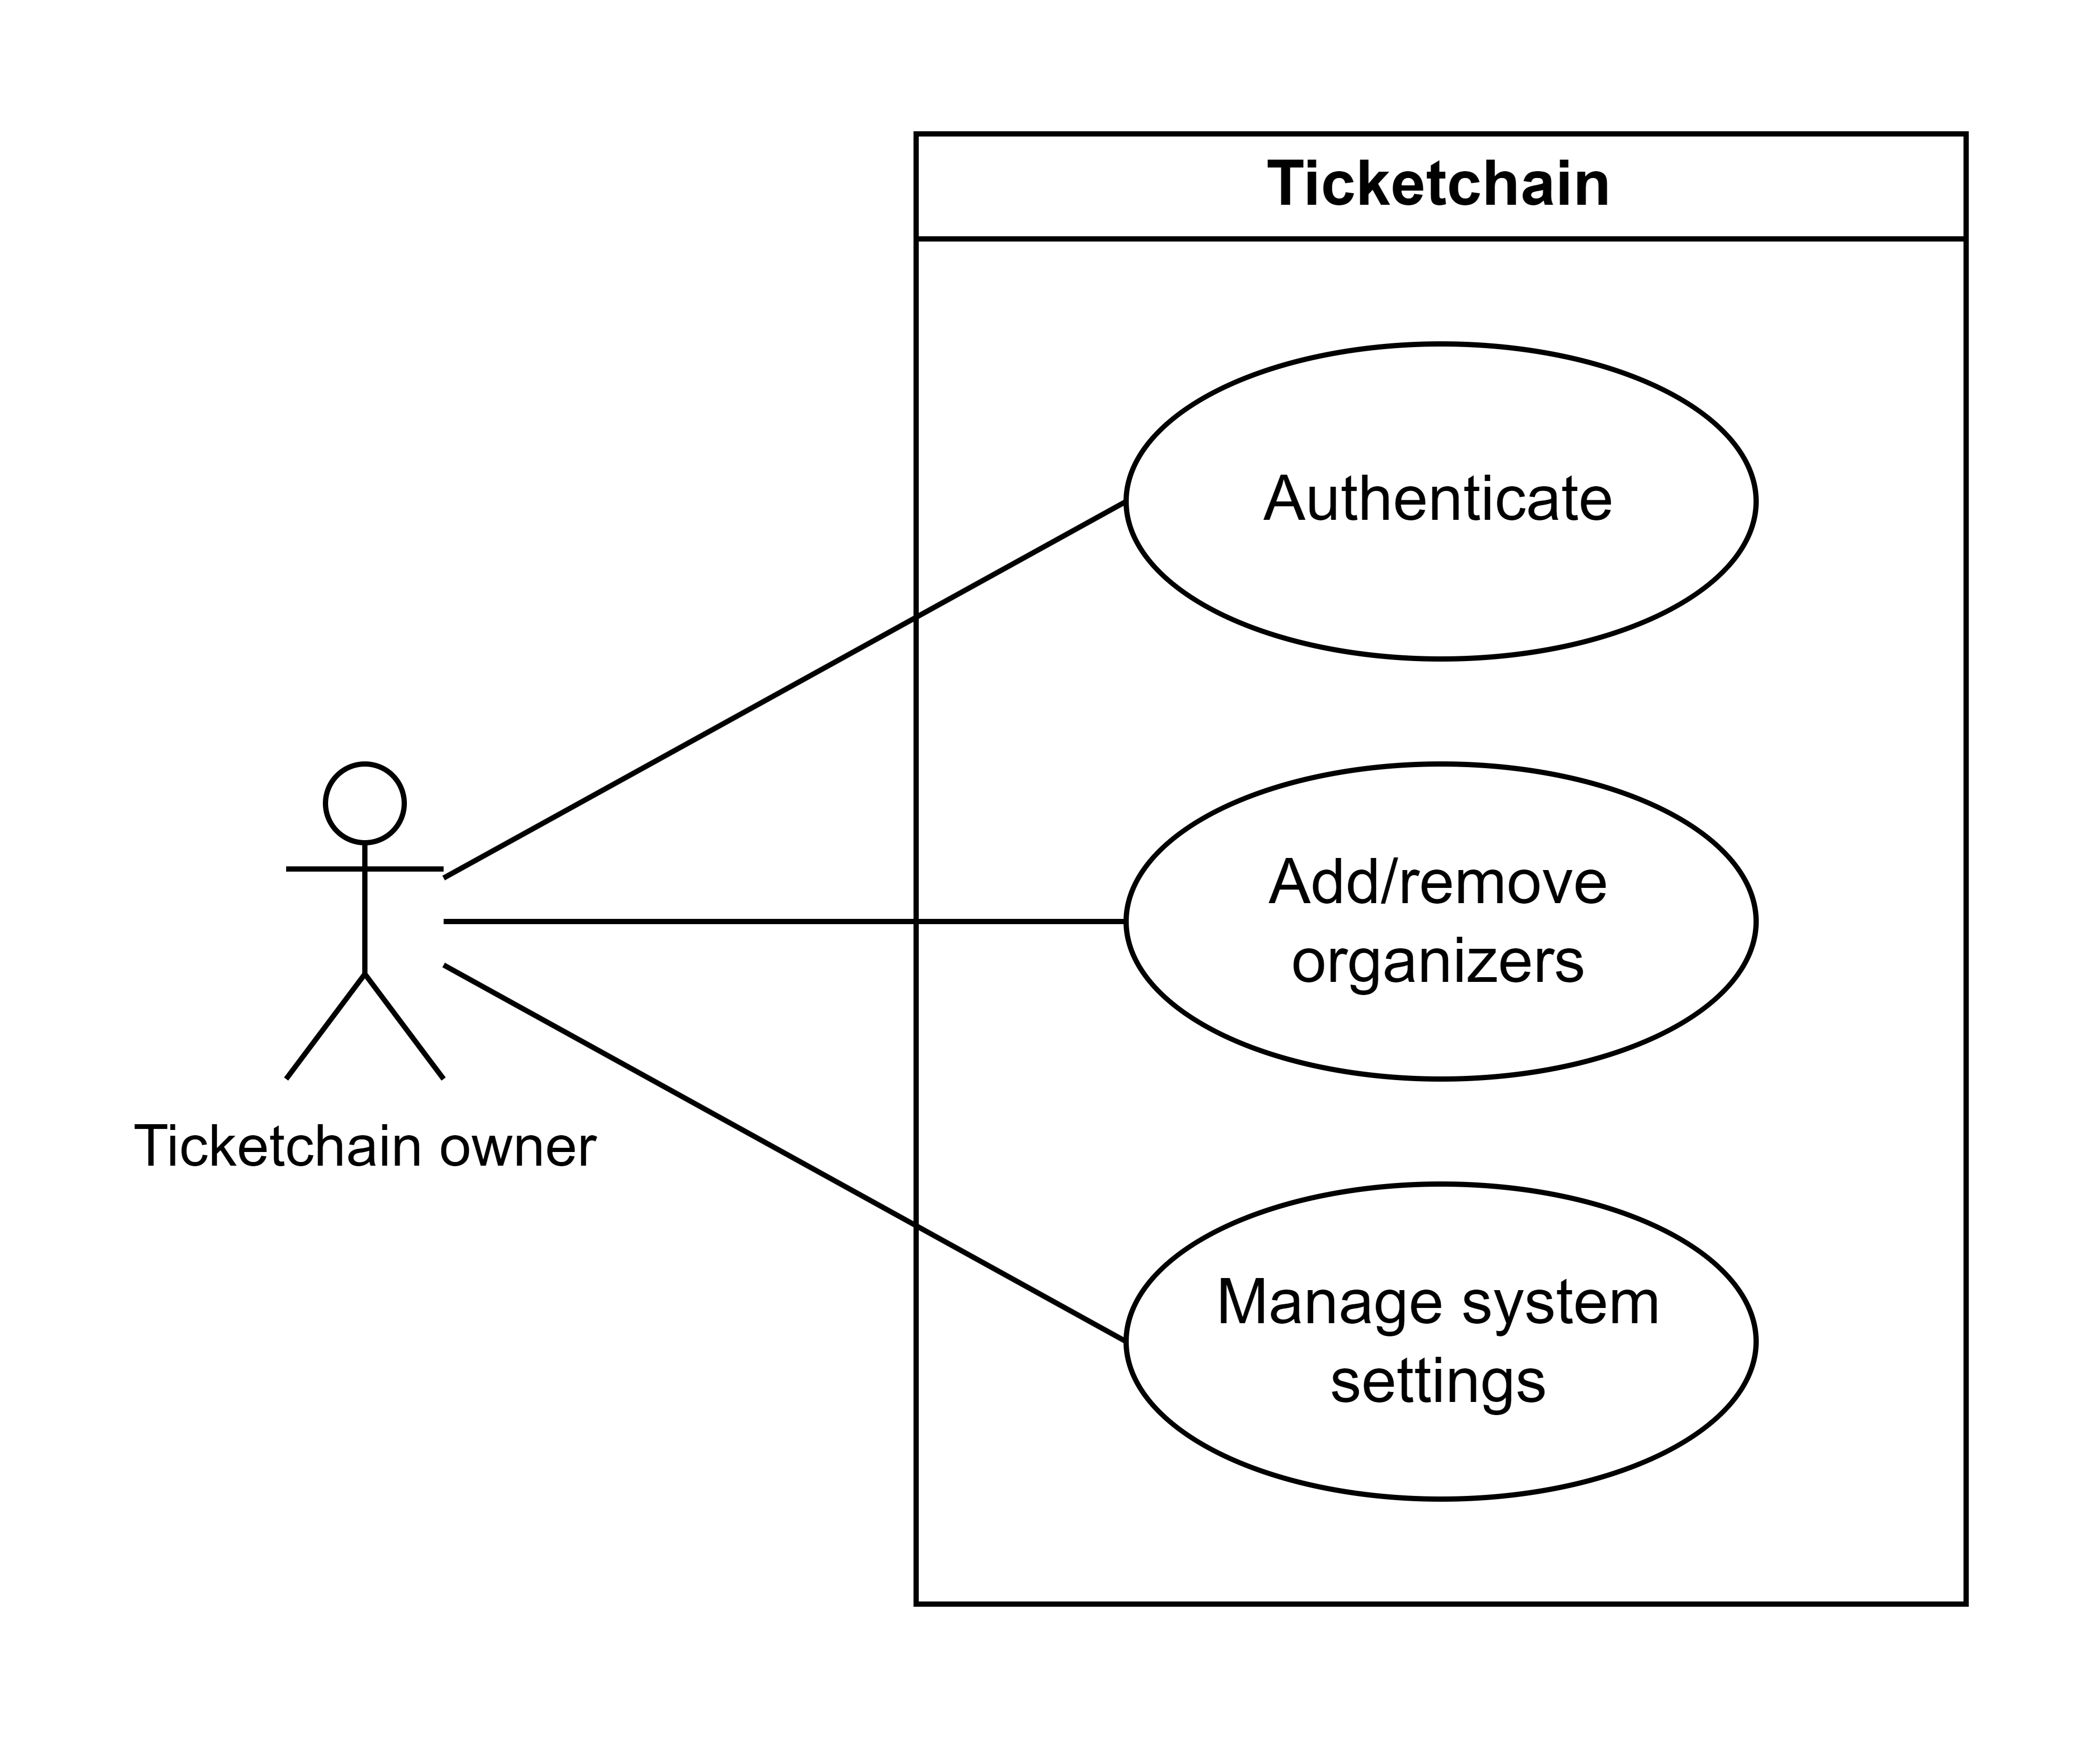
\includegraphics[width=0.5\textwidth]{Ticketchain owner use cases.png}
    \caption{Ticketchain Owner Use Cases}
    \label{fig:ticketchain_owner_use_cases}
\end{figure}

This control is essential to ensure that only authorized individuals have
access to the system. Additionally, the Ticketchain owner can manage system
settings, which are crucial for tailoring the system’s behavior to meet the
needs of organizers.

\subsection{Organizer}
\label{subsec:organizer}

As shown in Figure \ref{fig:organizer_use_cases}, the organizer has several key
use cases, including event creation and management.

\begin{figure}[H]
    \centering
    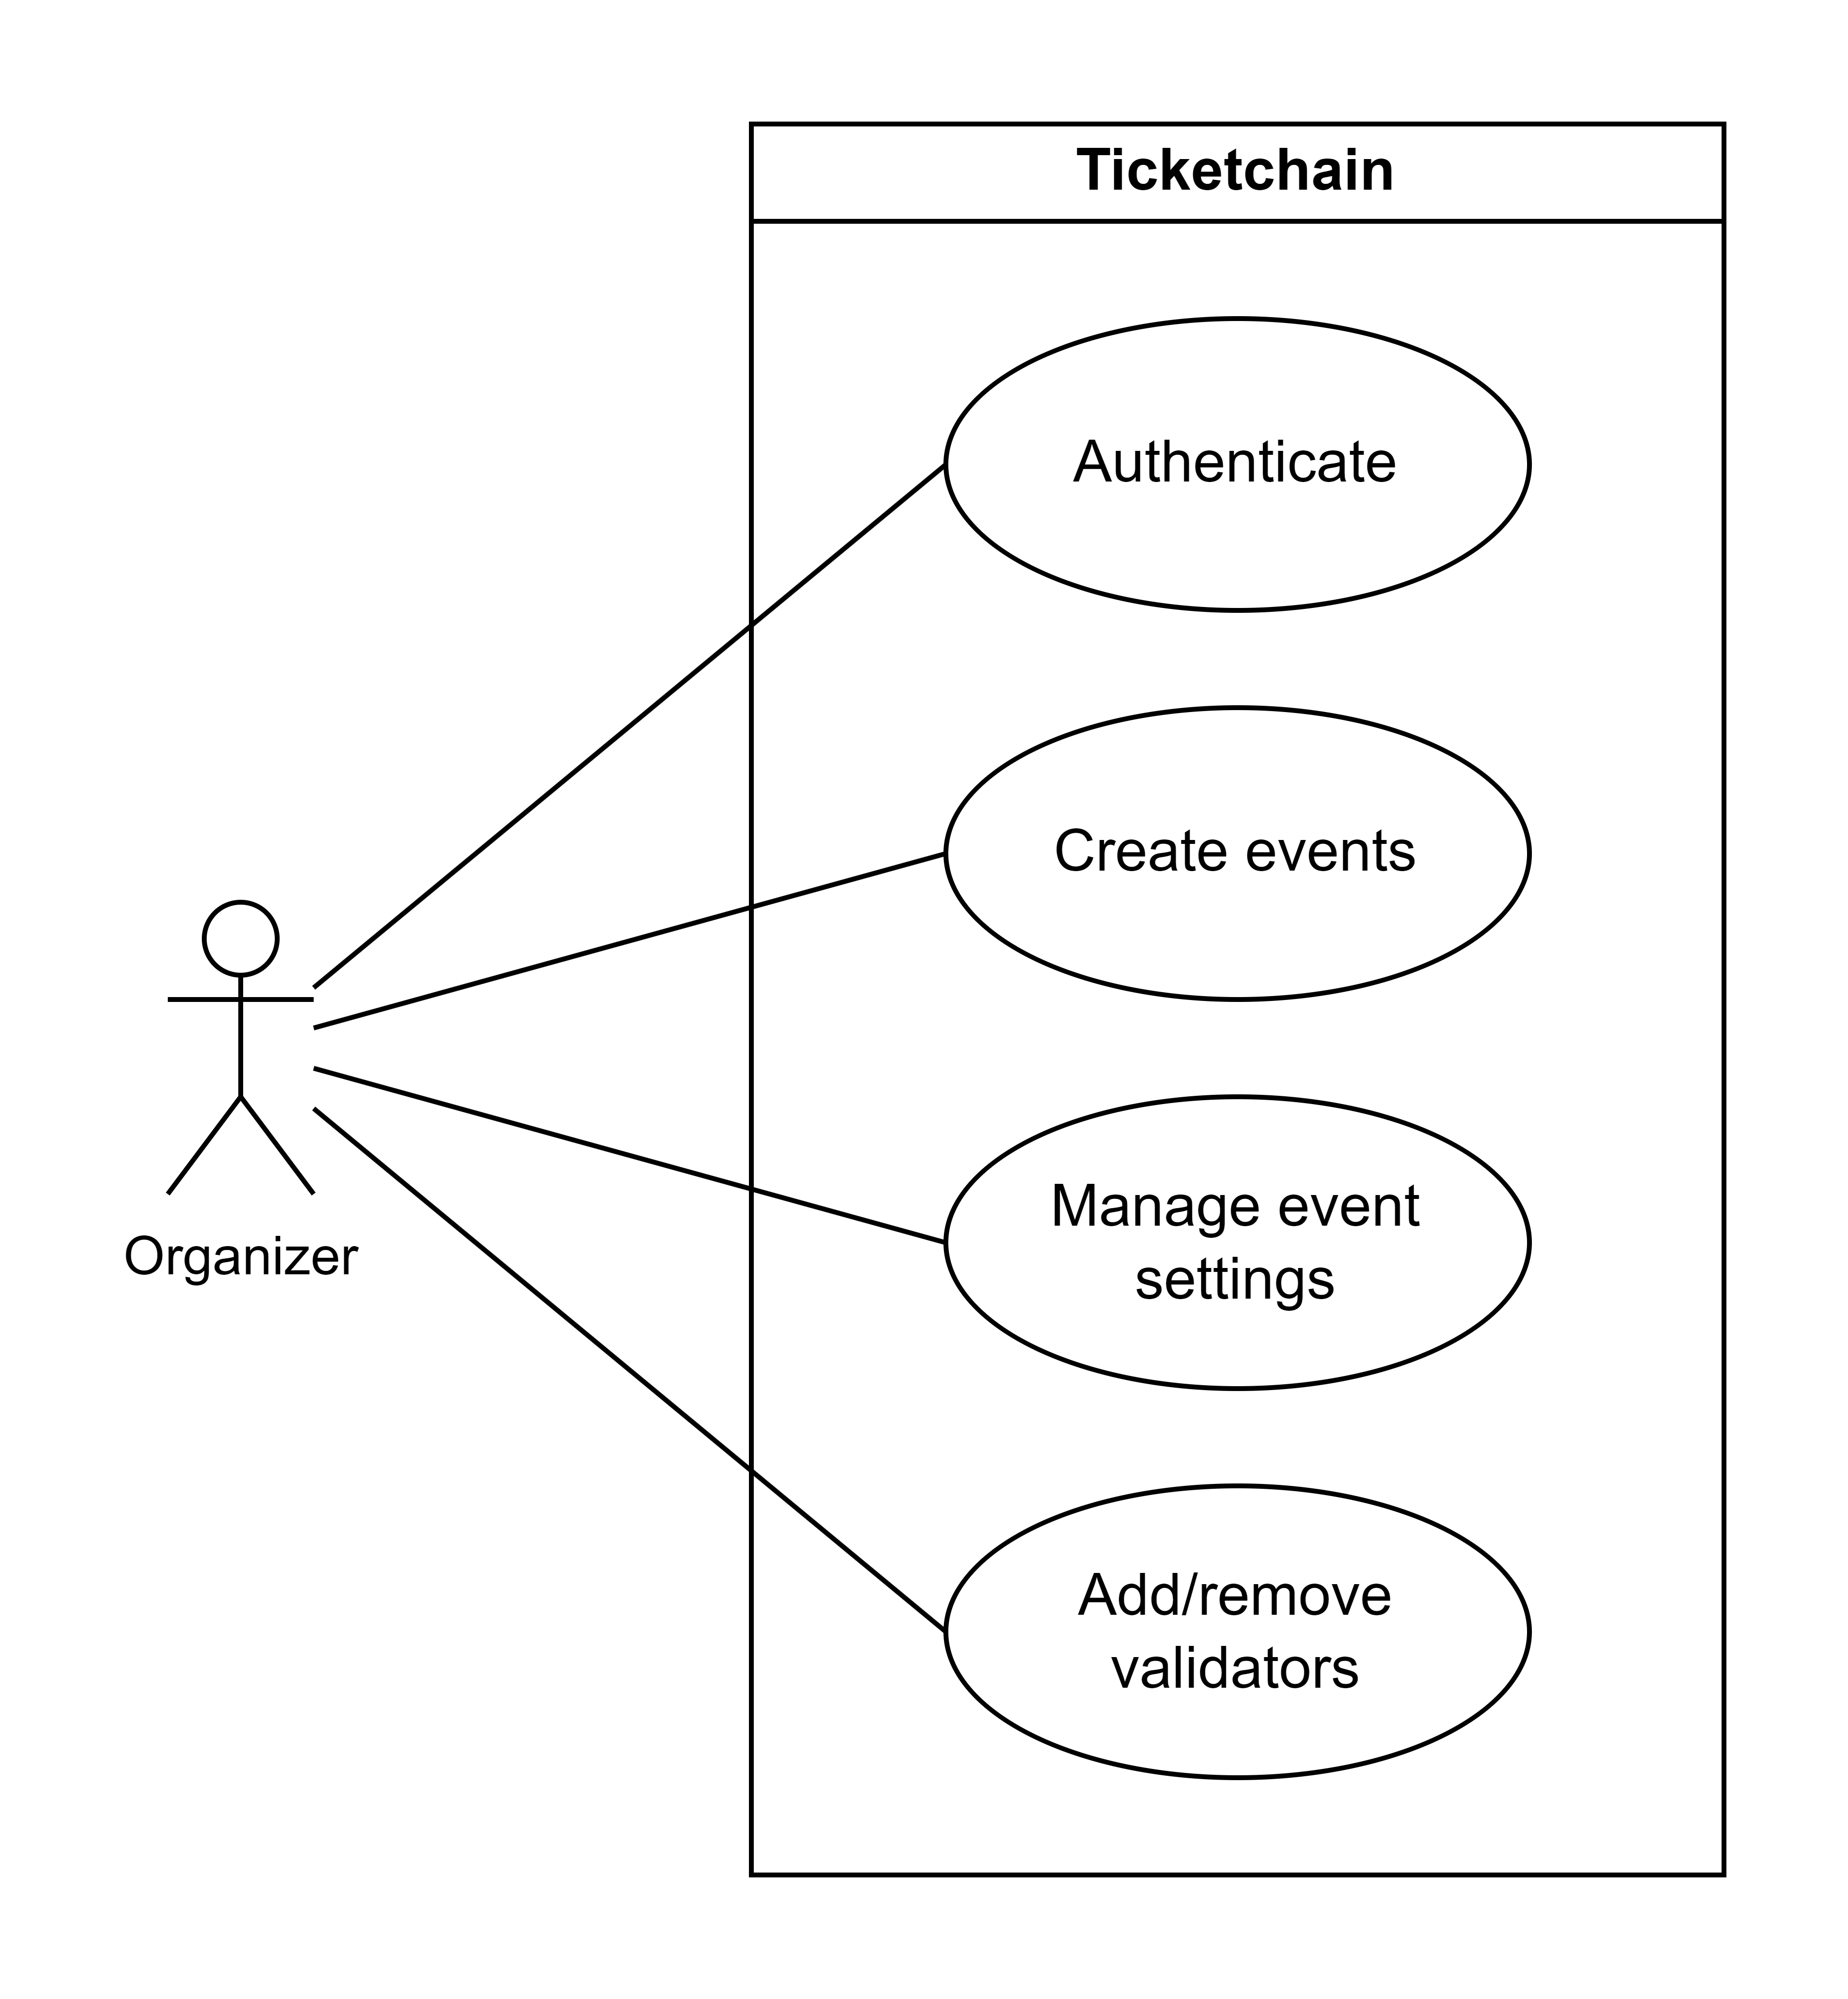
\includegraphics[width=0.5\textwidth]{Organizer use cases.png}
    \caption{Organizer Use Cases}
    \label{fig:organizer_use_cases}
\end{figure}

The organizer also oversees the selection of validators for each event,
ensuring that only authorized personnel can validate tickets. Furthermore, the
organizer can manage event settings, such as updating information or canceling
events when necessary.

\subsection{Validator}
\label{subsec:validator}

For validators, as illustrated in Figure \ref{fig:validator_use_cases}, the
primary use case is to validate users' tickets, allowing entry to the event.

\begin{figure}[H]
    \centering
    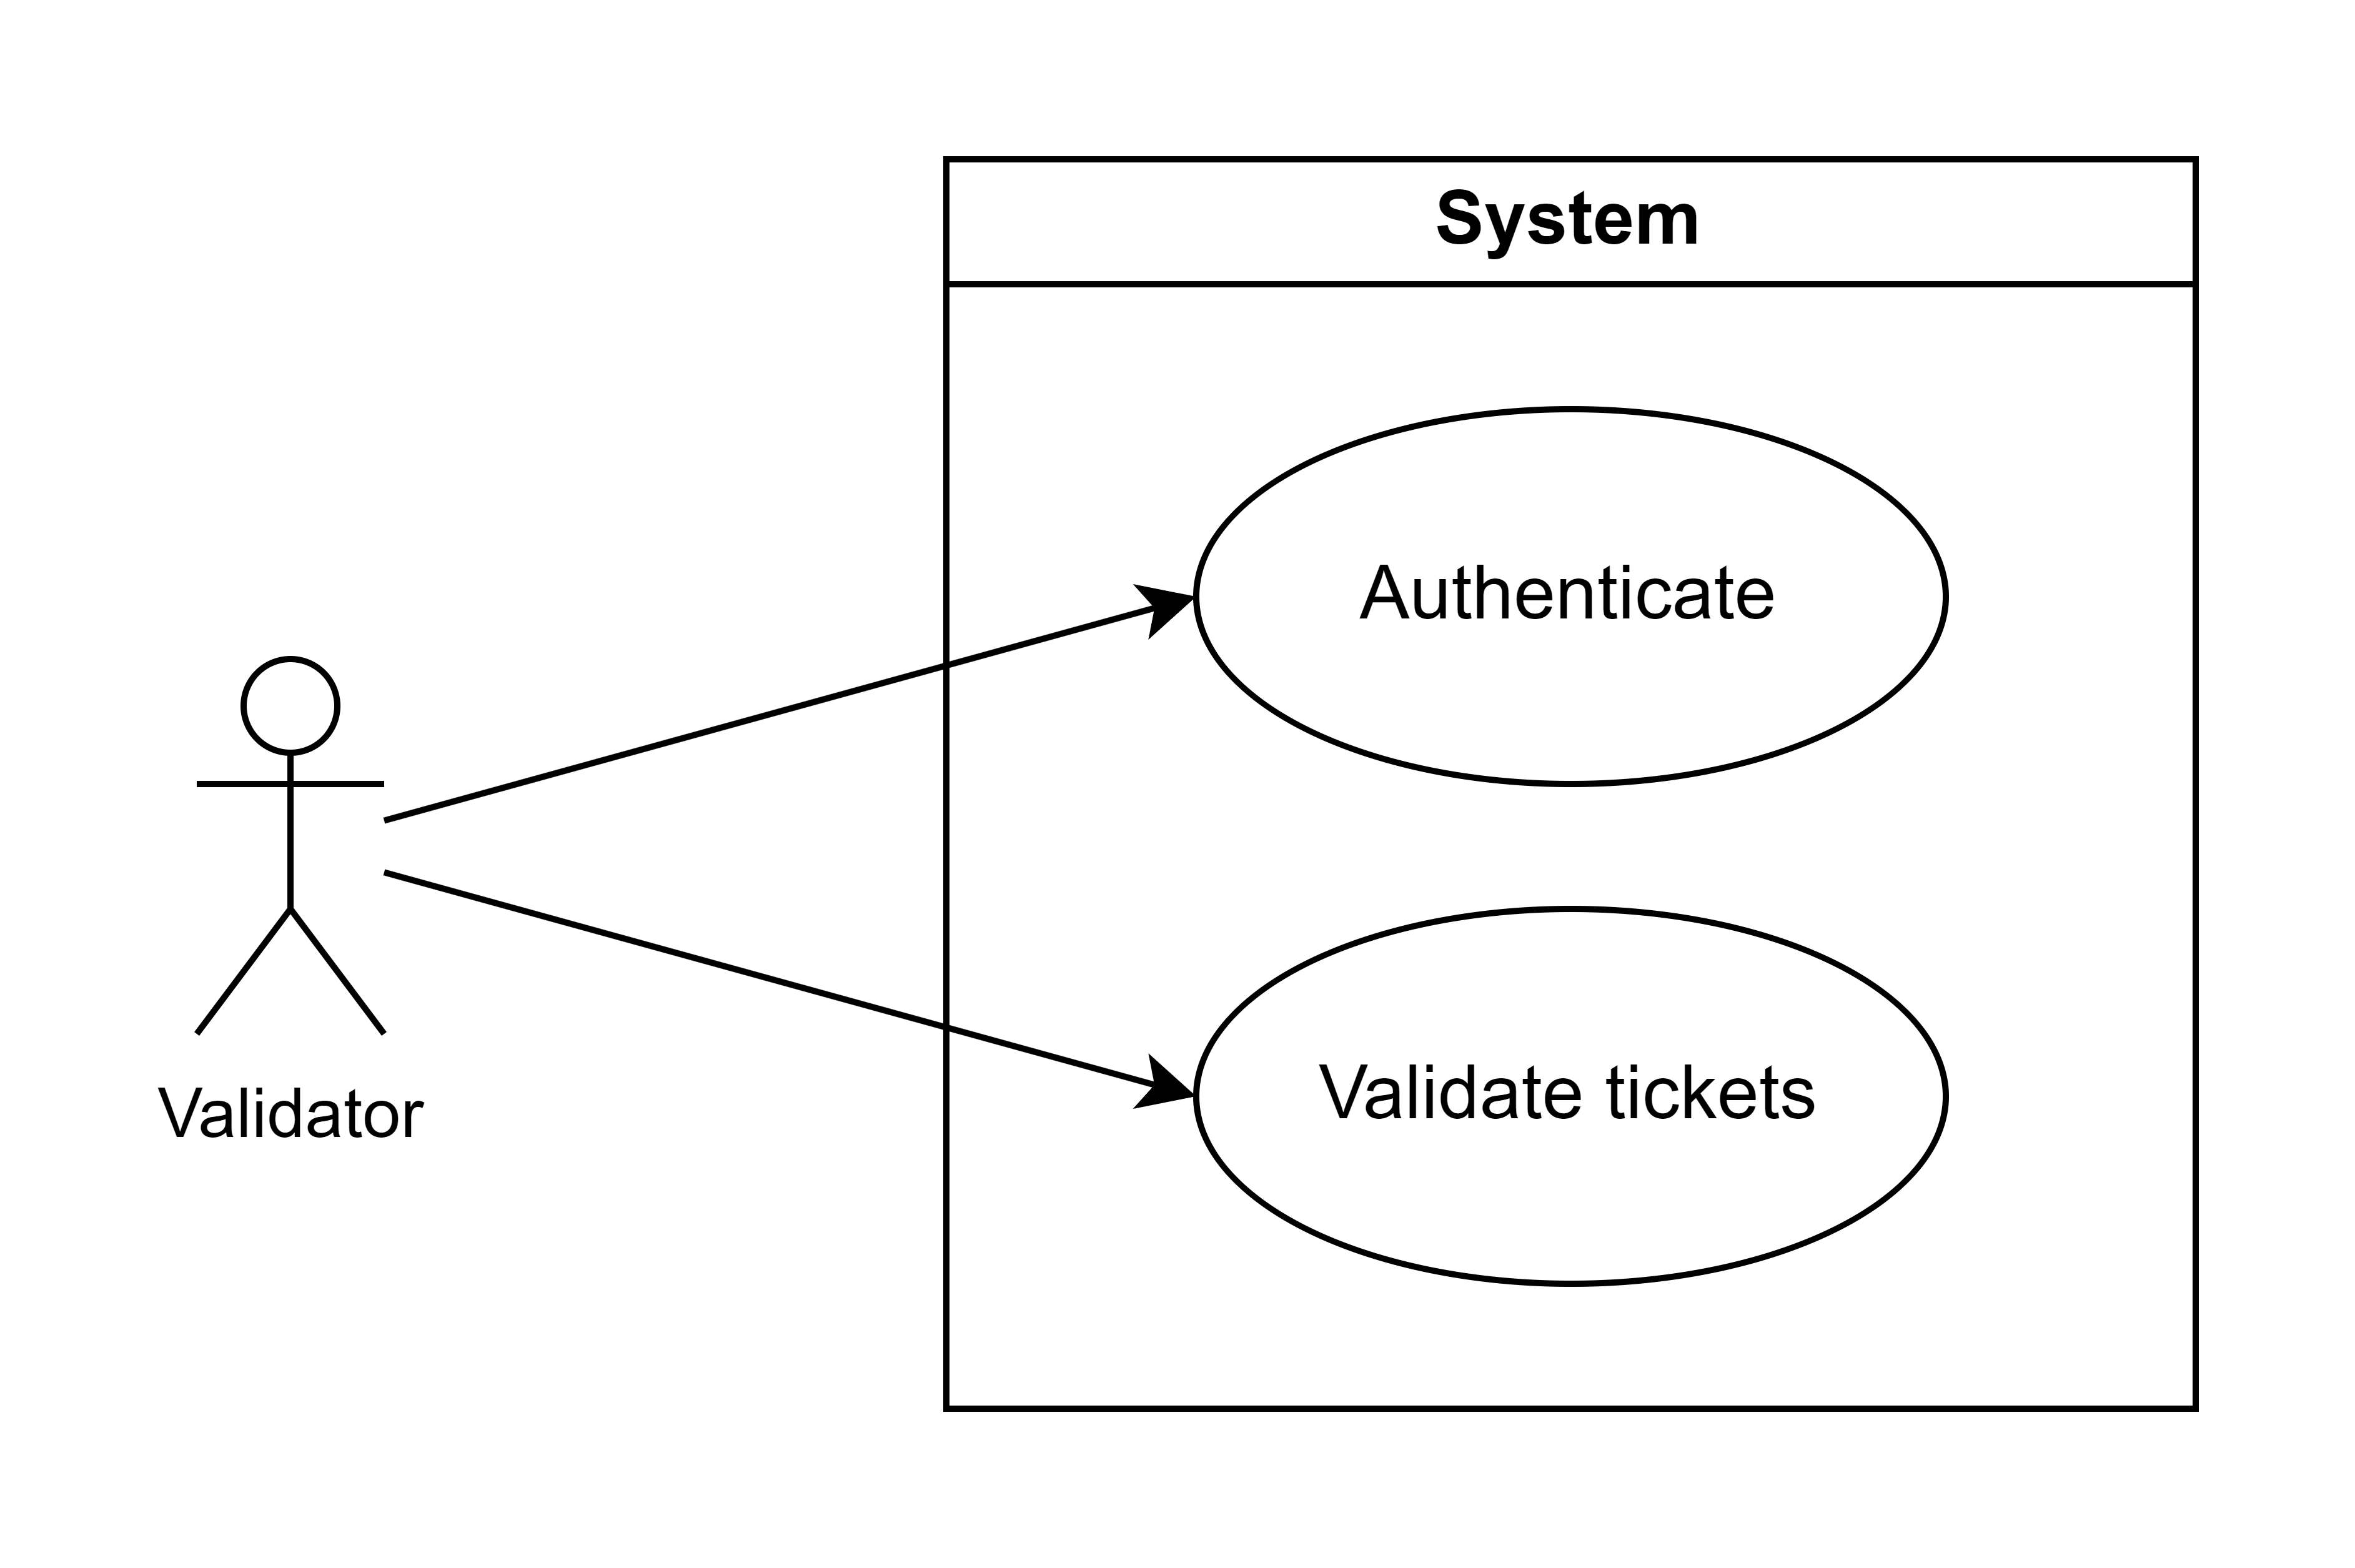
\includegraphics[width=0.5\textwidth]{Validator use cases.png}
    \caption{Validator Use Cases}
    \label{fig:validator_use_cases}
\end{figure}

This step is critical for maintaining security and ensuring that only users
with valid tickets can participate.

\subsection{Common User}
\label{subsec:common_user}

Figure \ref{fig:common_user_use_cases} presents the use cases for common users.

\begin{figure}[H]
    \centering
    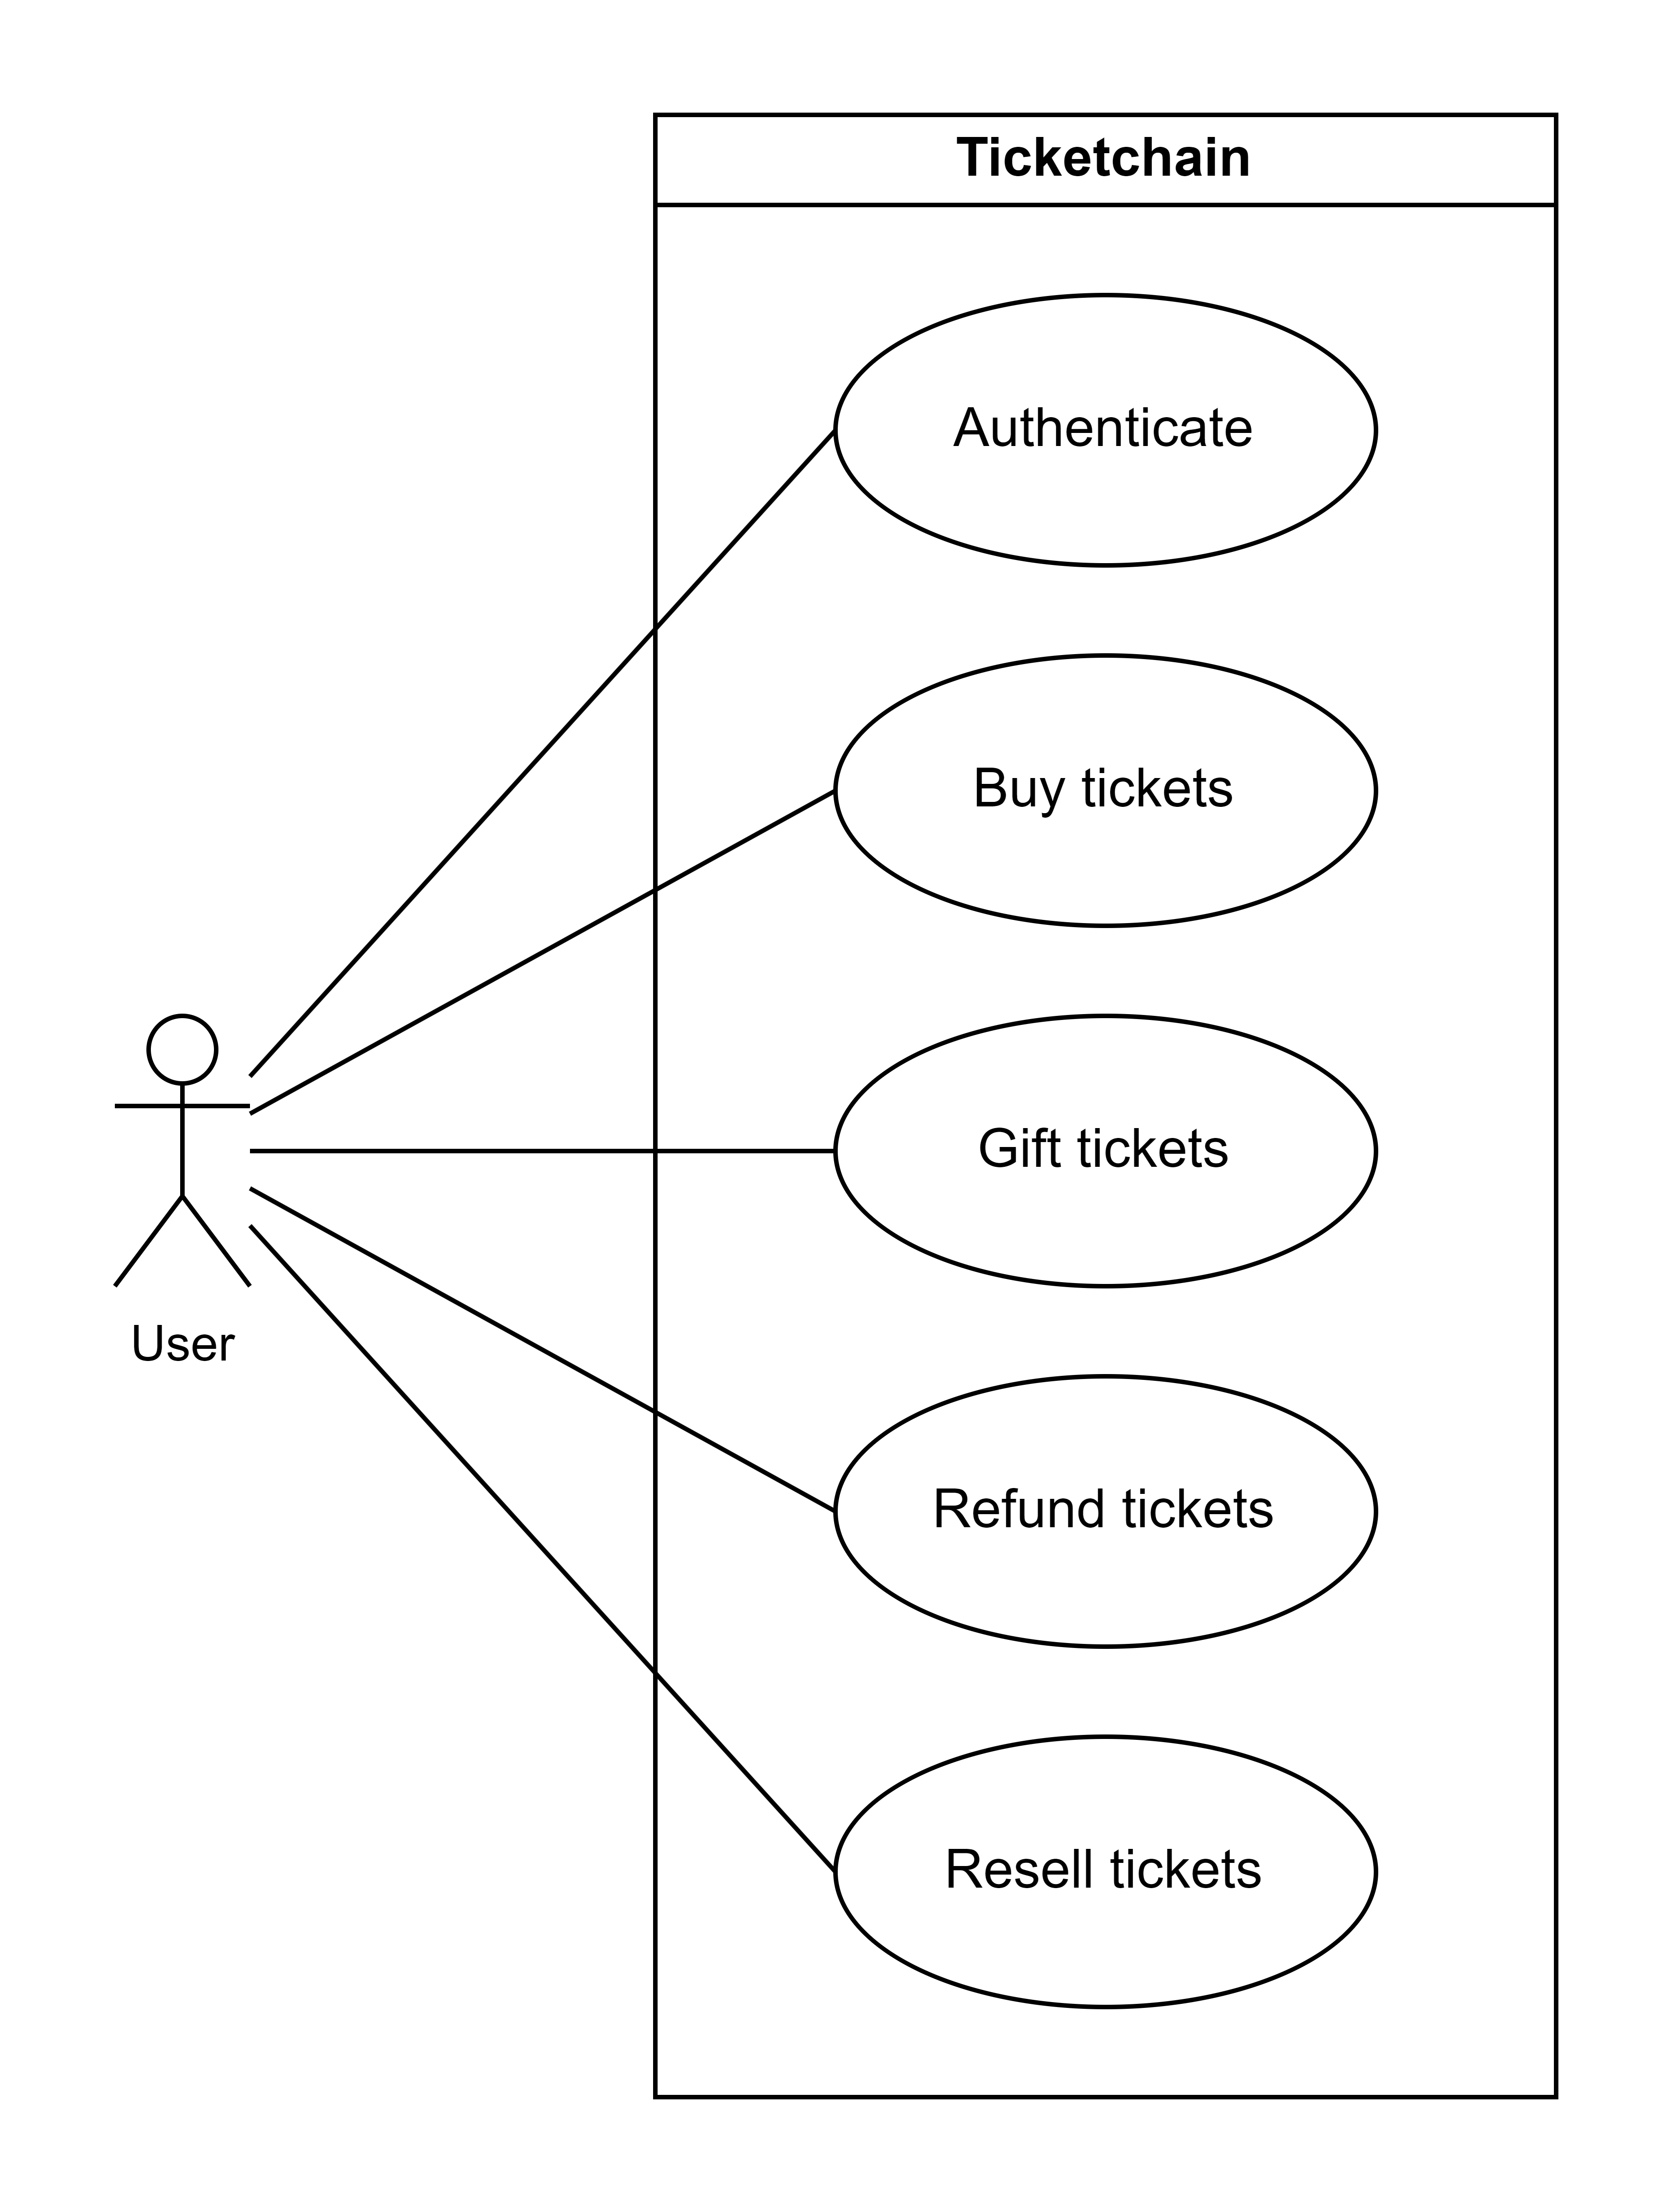
\includegraphics[width=0.5\textwidth]{Common user use cases.png}
    \caption{Common User Use Cases}
    \label{fig:common_user_use_cases}
\end{figure}

Users can purchase tickets, gift them to others, request refunds (depending on
event policies), and resell tickets (with the condition that they cannot sell
at a price higher than the original). These use cases provide users with the
flexibility to manage their tickets according to their preferences while
adhering to system regulations.

\section{Architecture}
\label{sec:architecture}

As this work is a blockchain-based project, the goal is to minimize the use of
traditional Web2 technologies, such as server-based backends and related
services. Instead, we aim to rely primarily on Web3 technologies to fully
understand the limitations and possibilities of adopting a blockchain-only
ecosystem. In the future, a hybrid approach combining both Web2 and Web3 could
offer significant advantages. The system architecture is depicted in Figure
\ref{fig:architecture}, illustrating how the various components of the project
interact, in line with the requirements discussed in previous sections.

\begin{figure}[H]
    \centering
    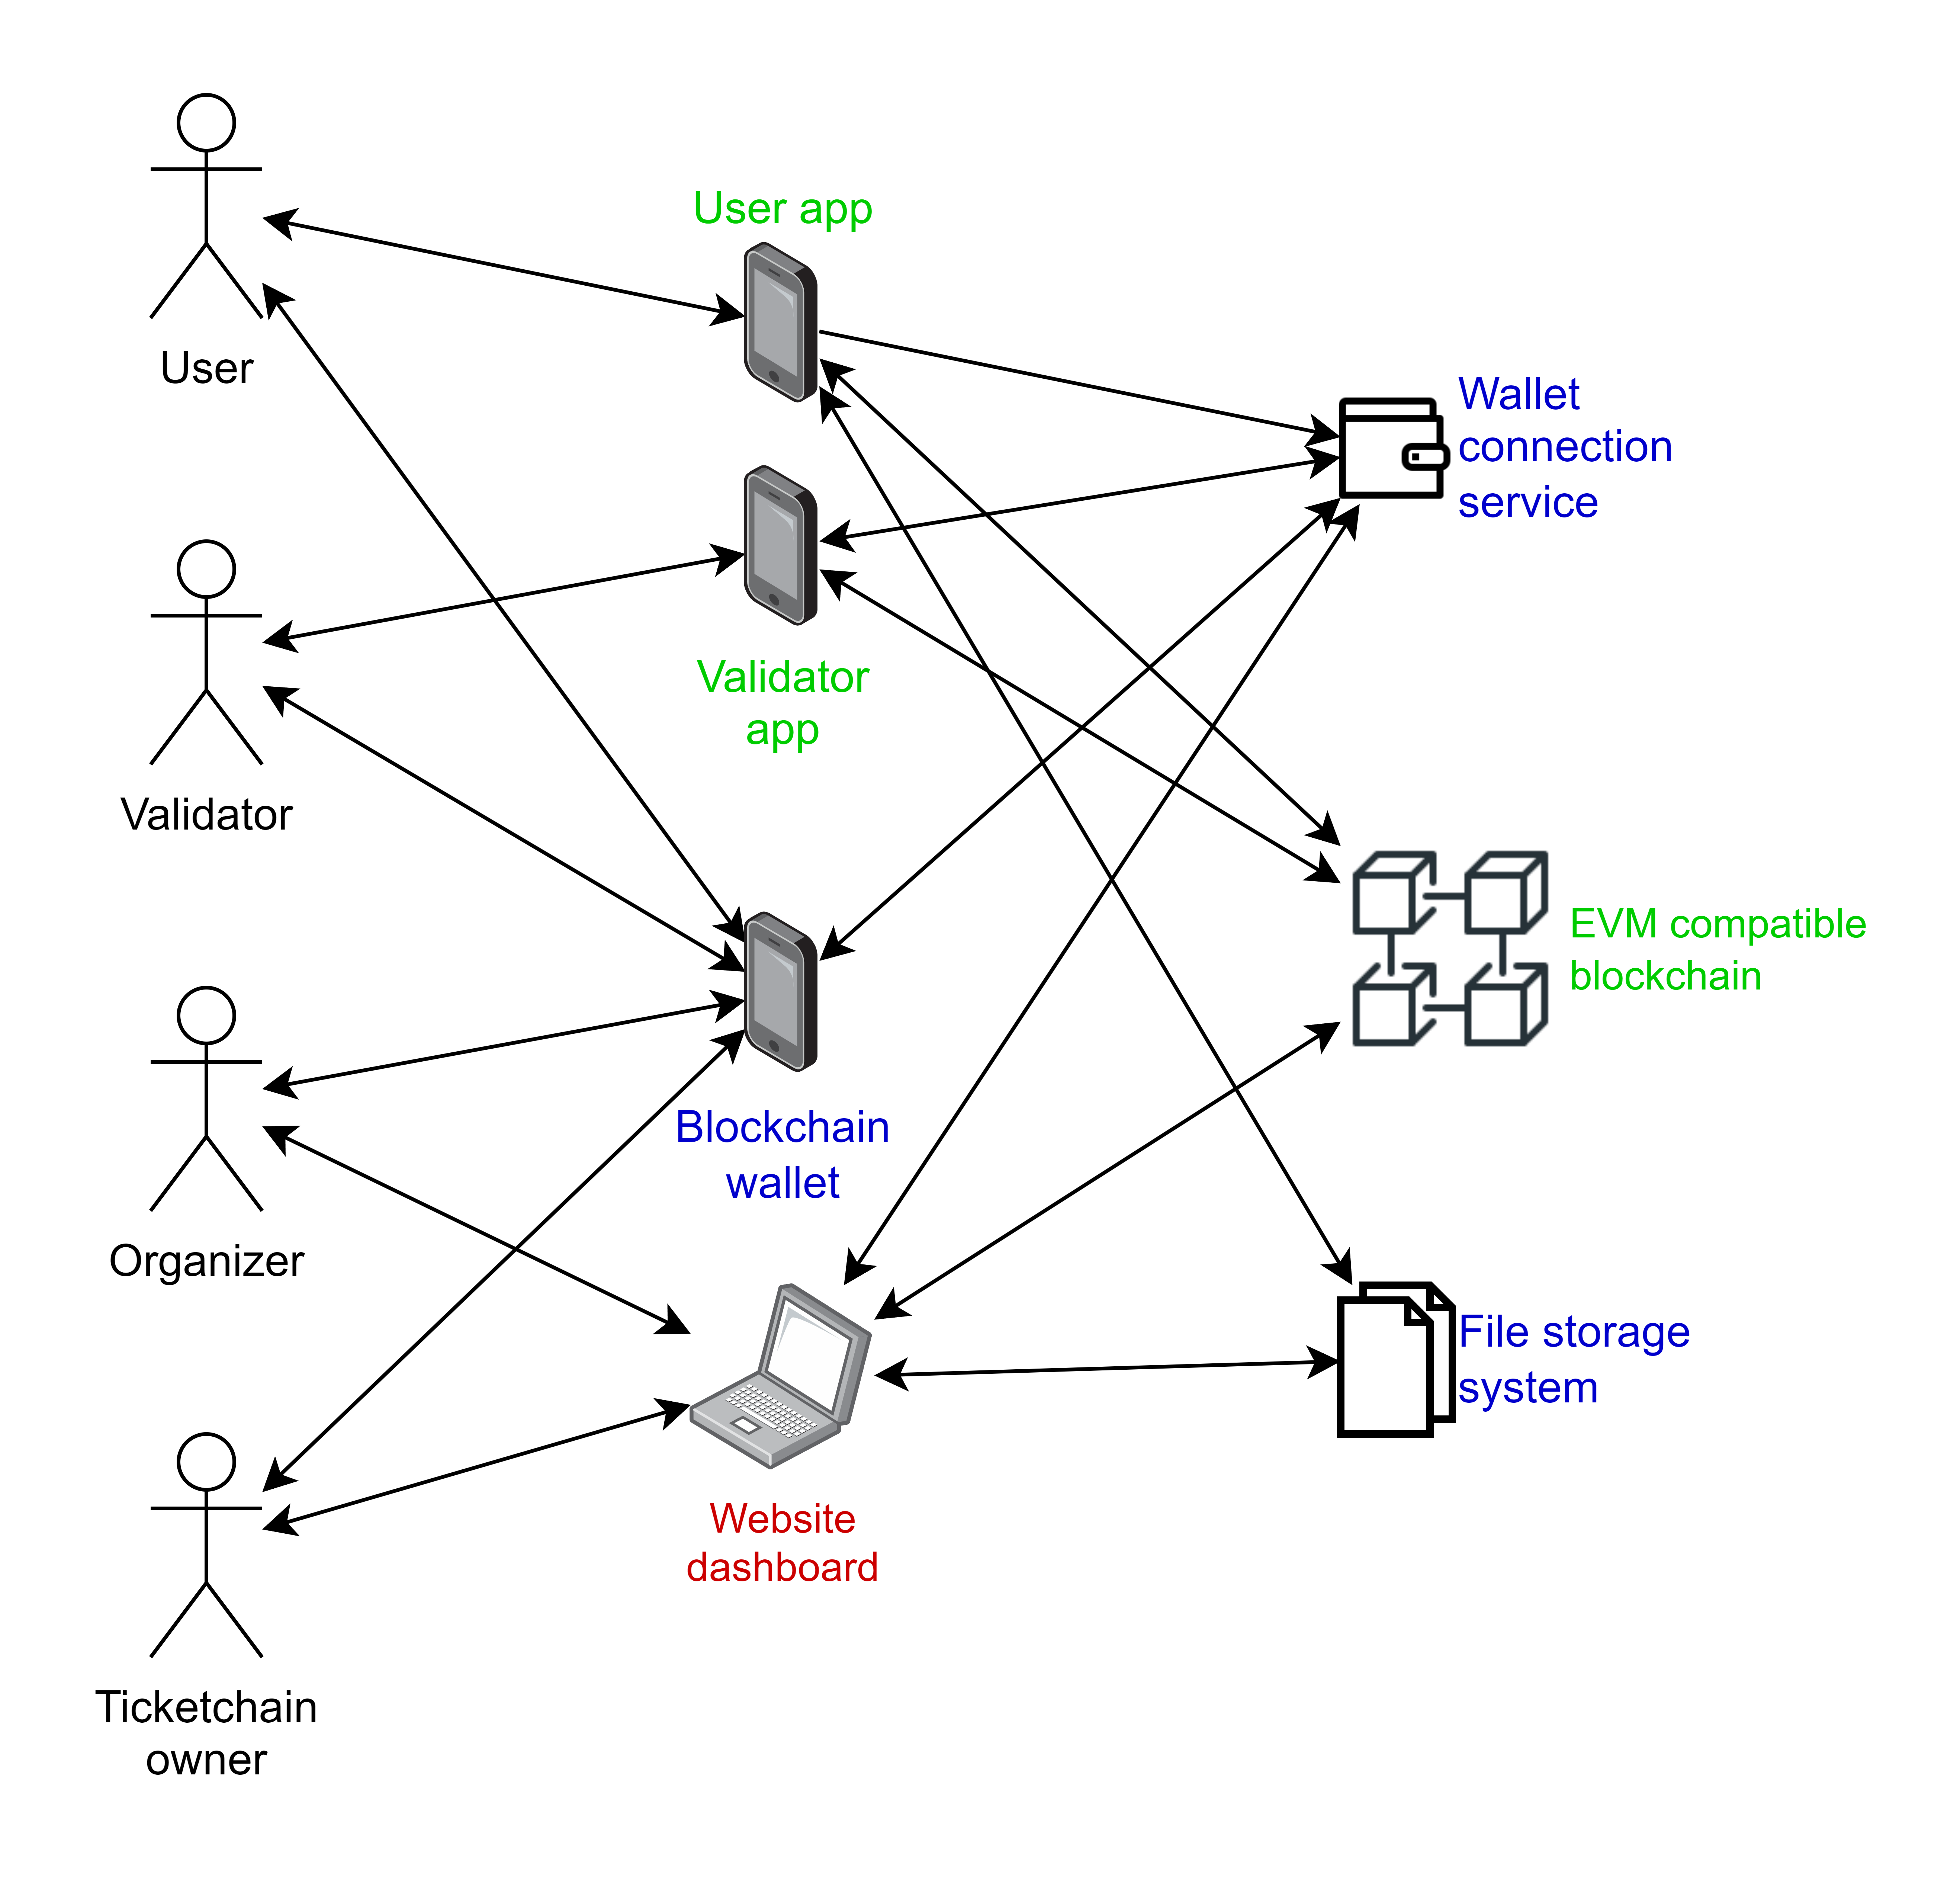
\includegraphics[width=\textwidth*2/3]{Architecture.png}
    \caption{System Architecture}
    \label{fig:architecture}
\end{figure}

The architecture includes two main mobile applications—one for regular users
and the other for validators—as well as a website dashboard for the Ticketchain
owner and event organizers to manage system settings and events.

The components highlighted in blue represent external services, while green
components denote those we are developing in the context of this project. The
red component, the website dashboard, has not yet been implemented due to time
constraints, so for now, interactions will occur directly with the smart
contract. Additionally, to streamline development, the two mobile applications
have been consolidated into a single app, allowing us to focus on the core
functionality.

As described in previous sections, all users must authenticate before accessing
the system. Instead of traditional email and password logins, authentication
will require wallet software to interact with the blockchain. Thus, a wallet
connection service is needed to link user wallets to the system.

Once authenticated, the system will interact with the smart contract to display
event-related information and update the status of events or tickets. The smart
contracts will be deployed on an EVM-compatible blockchain.

Regarding ticket images, a file storage system will be required. This serves to
store images associated to the tickets, because storing them on-chain is
expensive. Although image uploads will eventually be handled via the dashboard,
this feature is not yet implemented, necessitating manual uploads for now.


\pagebreak
\chapter{Implementation}
\label{ch:implementation}

[Brief introduction of the chapter]

\section{Mobile App}
\label{sec:mobile_app}

The mobile app is the main interface for the users to interact with the system,
where they can authenticate, see the events, and buy and manage tickets. It
will have a main page to check the events and a page for each event, where the
user can see the details and buy the tickets, and will also have a page to see
the tickets he owns.

We also made the validator logic in the same app to simplify the process, so we
don't have to make a separate app for the validators, however in a real
scenario we would have separate apps.

The app will be developed using the Flutter framework, which is a
cross-platform framework that allows us to build apps for Android and iOS from
a single codebase. It's made by Google and it's very popular for its ease of
use and performance.

\subsection{Authentication}
\label{subsec:authentication}

The Figure \ref{fig:authentication_page} shows the starting point of the app
that separates the authentication of the common users from the validators.

\begin{figure}[H]
	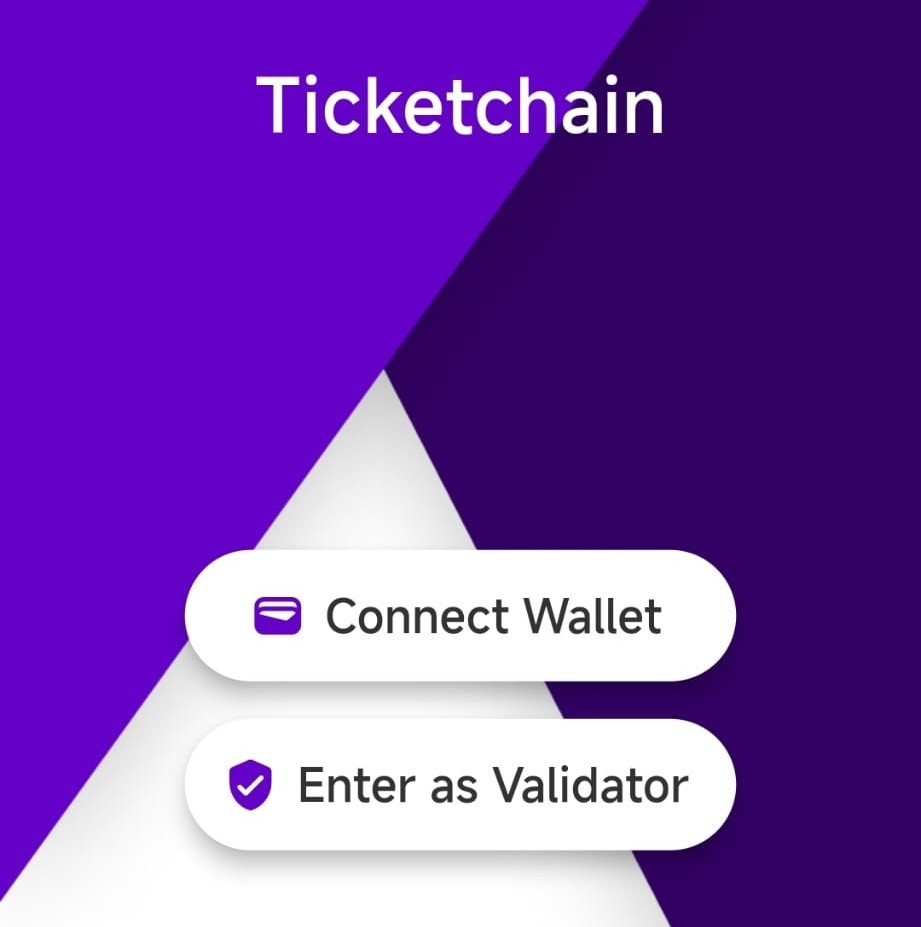
\includegraphics[width=\textwidth/3,frame]{Authentication page.jpg}
	\centering
	\caption{Authentication page}
	\label{fig:authentication_page}
\end{figure}

To authenticate the users, we will use the
\href{https://walletconnect.com/}{Wallet Connect} service, which supports a
variety of wallets to interact with. What this service does is establishes a
connection between the app and a wallet, so that when a function needs to be
called, the wallet receives the prompt and signs the transaction after the
user's approval.

The Figure \ref{fig:wallet_connect_prompt} shows what happens when we try to
authenticate as common users which triggers the Wallet Connect service. This
lists all the wallets that are supported by the service and the user can choose
the one he uses.

\begin{figure}[H]
	\includegraphics[width=\textwidth/3,frame]{Wallet connect prompt.jpg}
	\centering
	\caption{Wallet connect prompt}
	\label{fig:wallet_connect_prompt}
\end{figure}

After choosing one, the wallet app will open automatically and the user will
have to approve the connection, as the Figure \ref{fig:metamask_connect} shows.
We're using \href{https://metamask.io/}{MetaMask} as the external blockchain
wallet, which is the most popular blockchain wallet and it's available as a
browser extension and as a mobile app. To use it, you just have to create a
wallet there and you'll be all set to start interacting with the app.

\begin{figure}[H]
	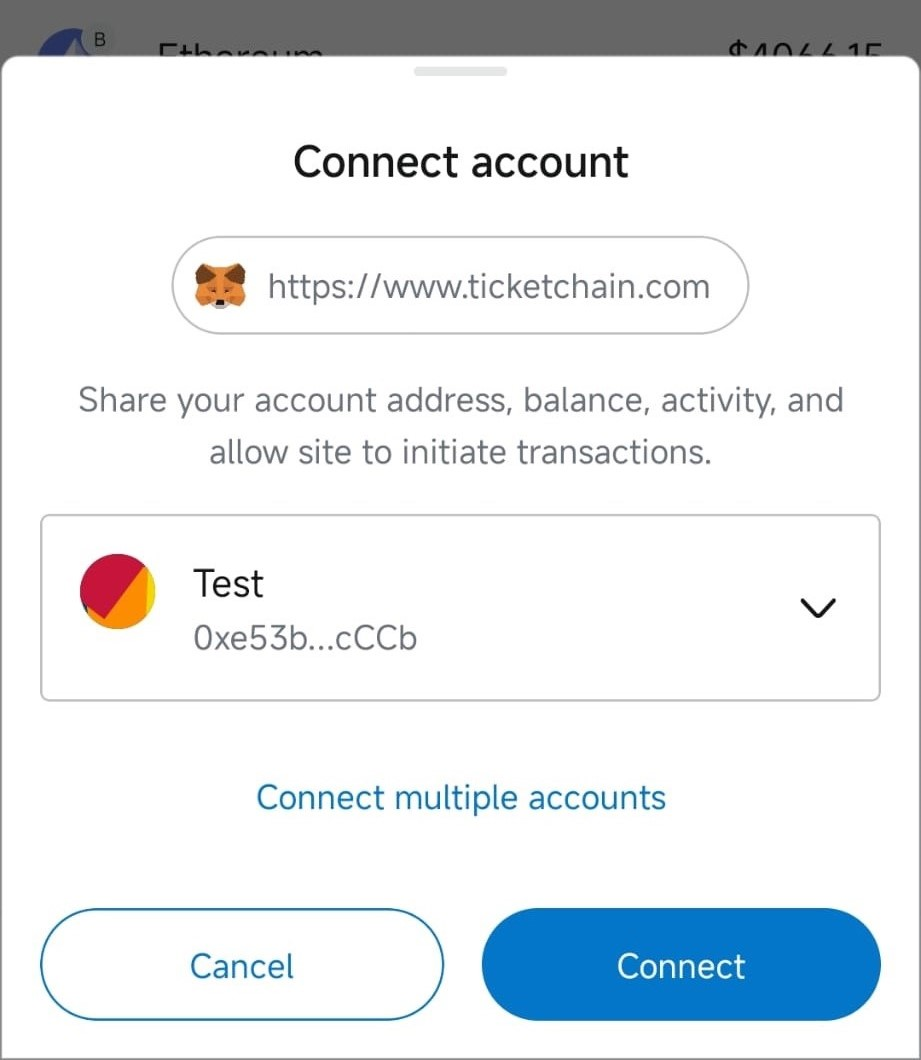
\includegraphics[width=\textwidth/3,frame]{MetaMask connect.jpg}
	\centering
	\caption{MetaMask connect}
	\label{fig:metamask_connect}
\end{figure}

The authentication is a one-time process, so the user doesn't have to do this
every time he wants to interact with the app. Basically when a connection is
established, the next time the app tries to reconnect to the wallet, it will
skip the prompt.

\subsection{Events}
\label{subsec:events}

After the common user authenticates, he will be redirected to the main page of
the app, where he can see the events that are available. The Figure
\ref{fig:main_page} shows the main page of the app, where the user can see the
events and search for them.

\begin{figure}[H]
	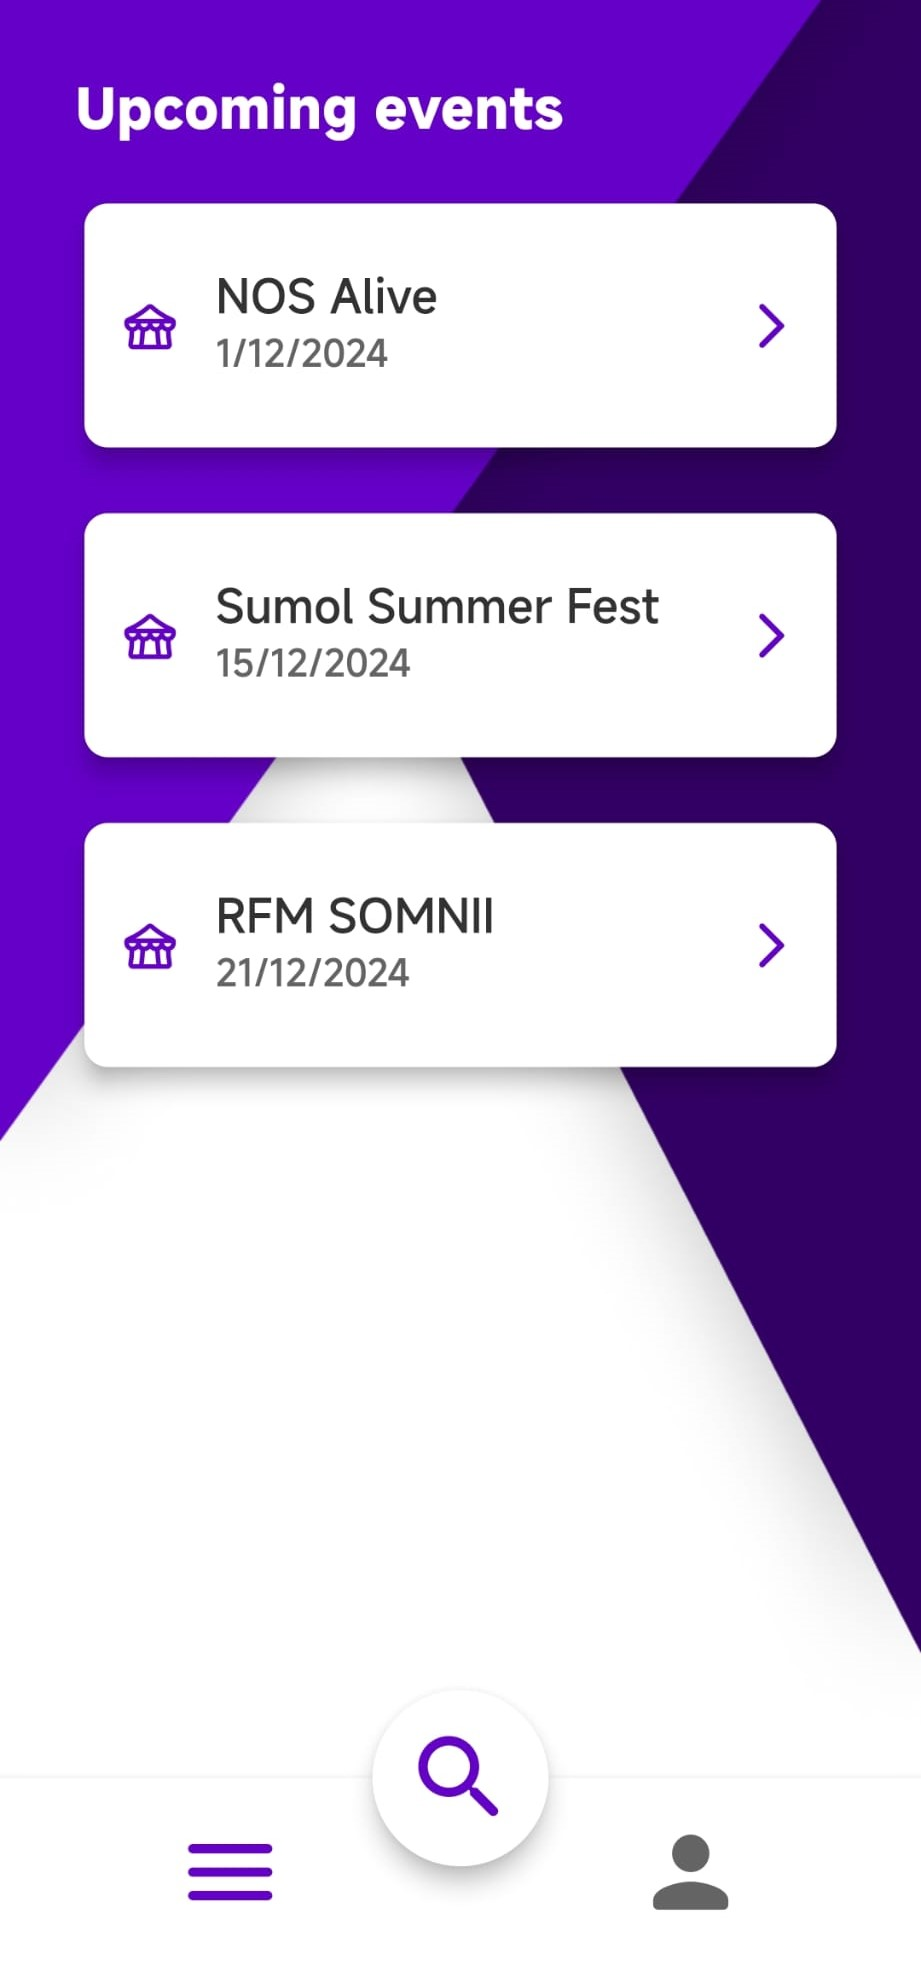
\includegraphics[width=\textwidth/3,frame]{Main page.jpg}
	\centering
	\caption{Main page}
	\label{fig:main_page}
\end{figure}

When clicking on one of the events, the user will be redirected to the event
page. The Figure \ref{fig:event_page} shows the event page, where the user can
see the details of the event and the packages available.

\begin{figure}[H]
	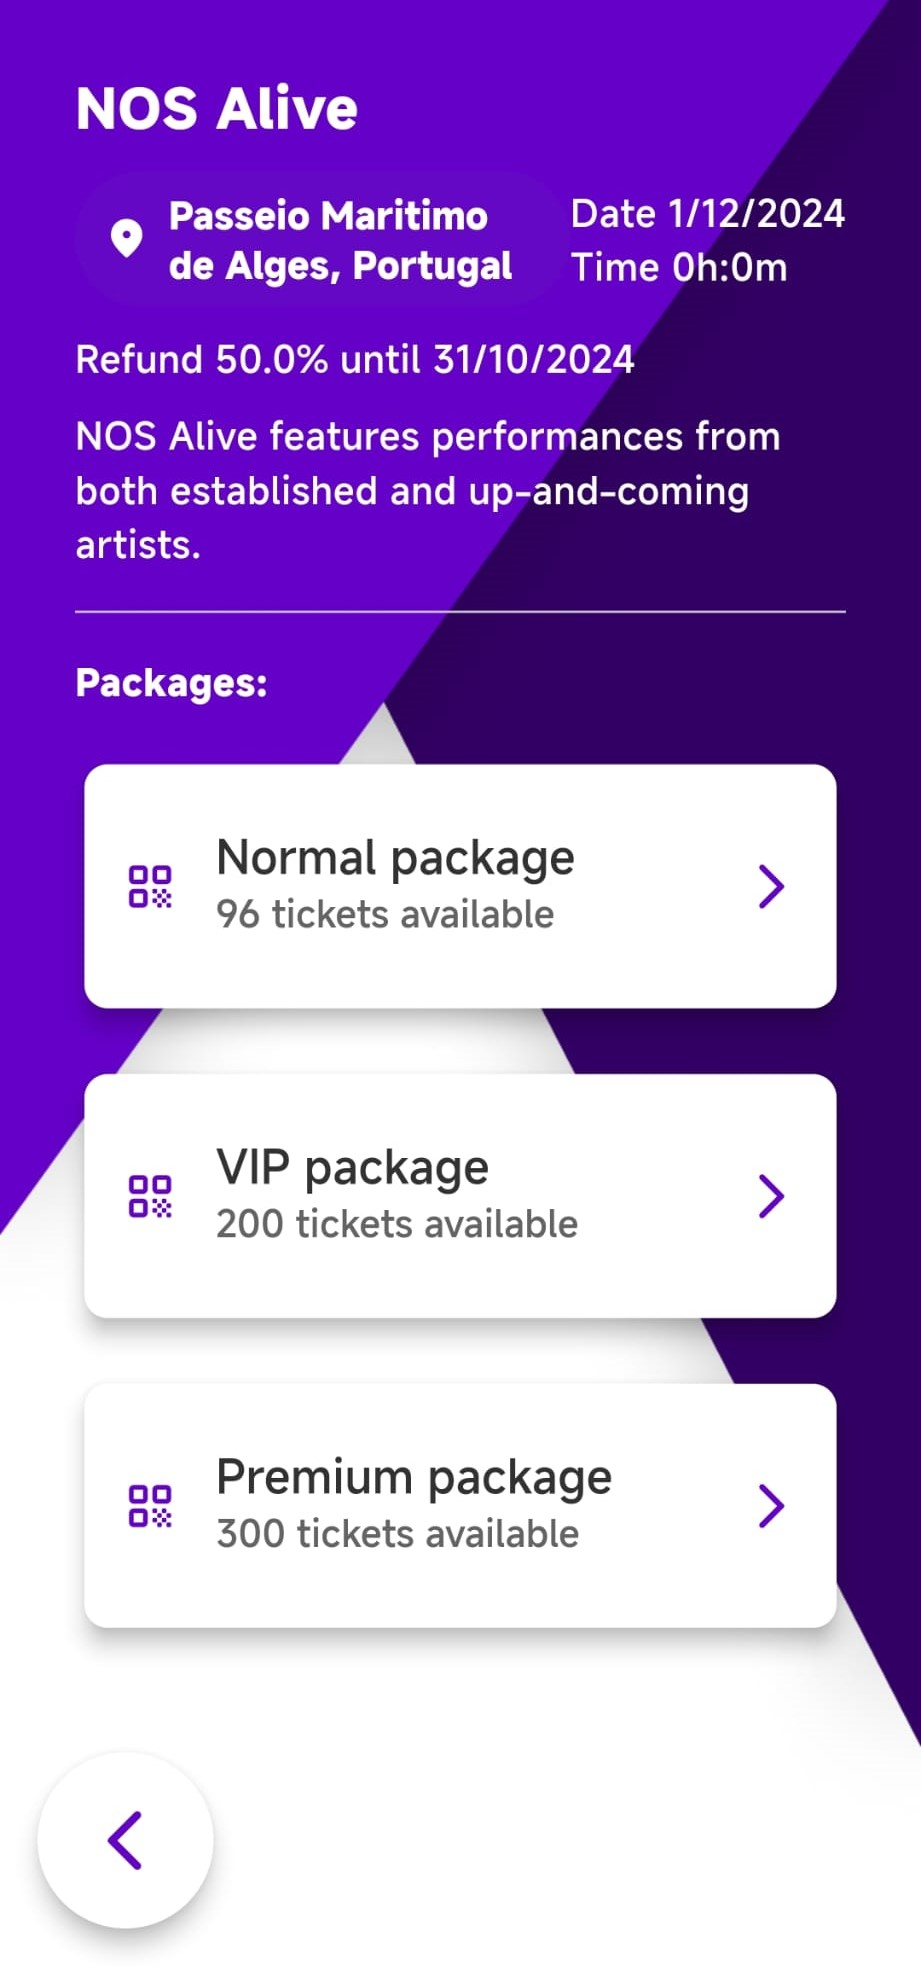
\includegraphics[width=\textwidth/3,frame]{Event page.jpg}
	\centering
	\caption{Event page}
	\label{fig:event_page}
\end{figure}

The user sees the name, description, location, date, packages and even the
refund information. When the user taps on the package he wants to buy, the
prompt shown in the Figure \ref{fig:buy_tickets_prompt} appears, where the user
can choose the amount of tickets he wants to buy. We went with this approach of
only choosing the amount of tickets to buy, but in the future a feature like
seat selection could be implemented.

\begin{figure}[H]
	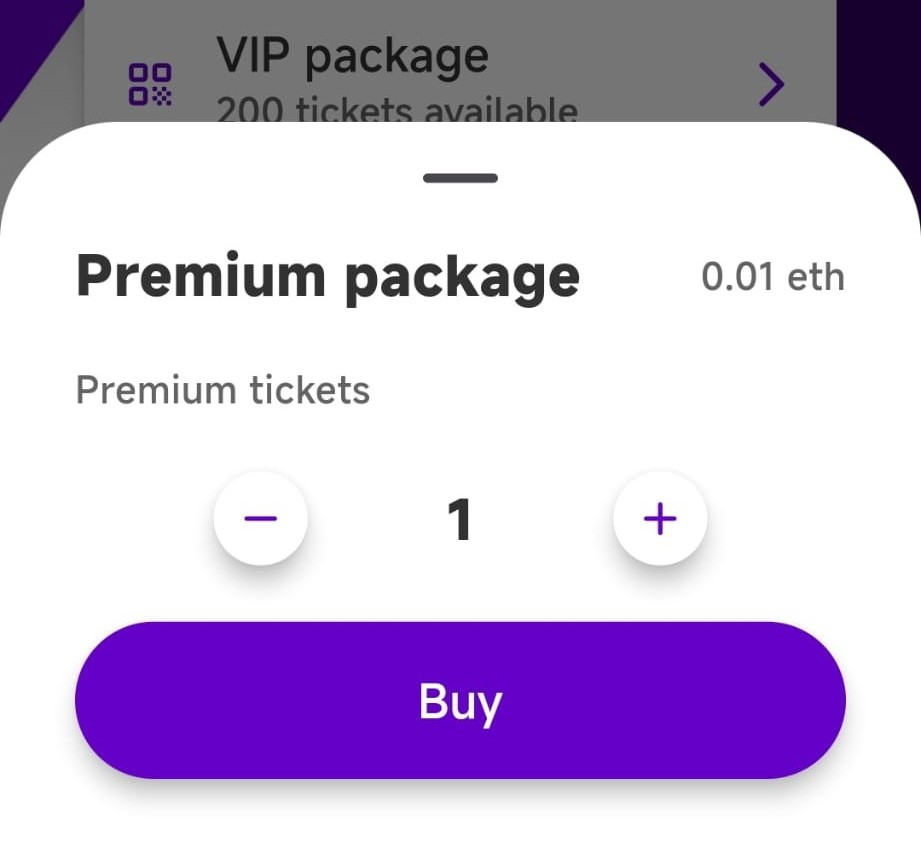
\includegraphics[width=\textwidth/3,frame]{Buy tickets prompt.jpg}
	\centering
	\caption{Buy tickets prompt}
	\label{fig:buy_tickets_prompt}
\end{figure}

The user can then confirm the purchase, and the wallet will prompt the user to
sign the transaction, as shown in the Figure
\ref{fig:metamask_transaction_prompt}. It displays the amount of money the user
has to pay, to which address he's interacting with, and the total cost to
execute the transaction.

\begin{figure}[H]
	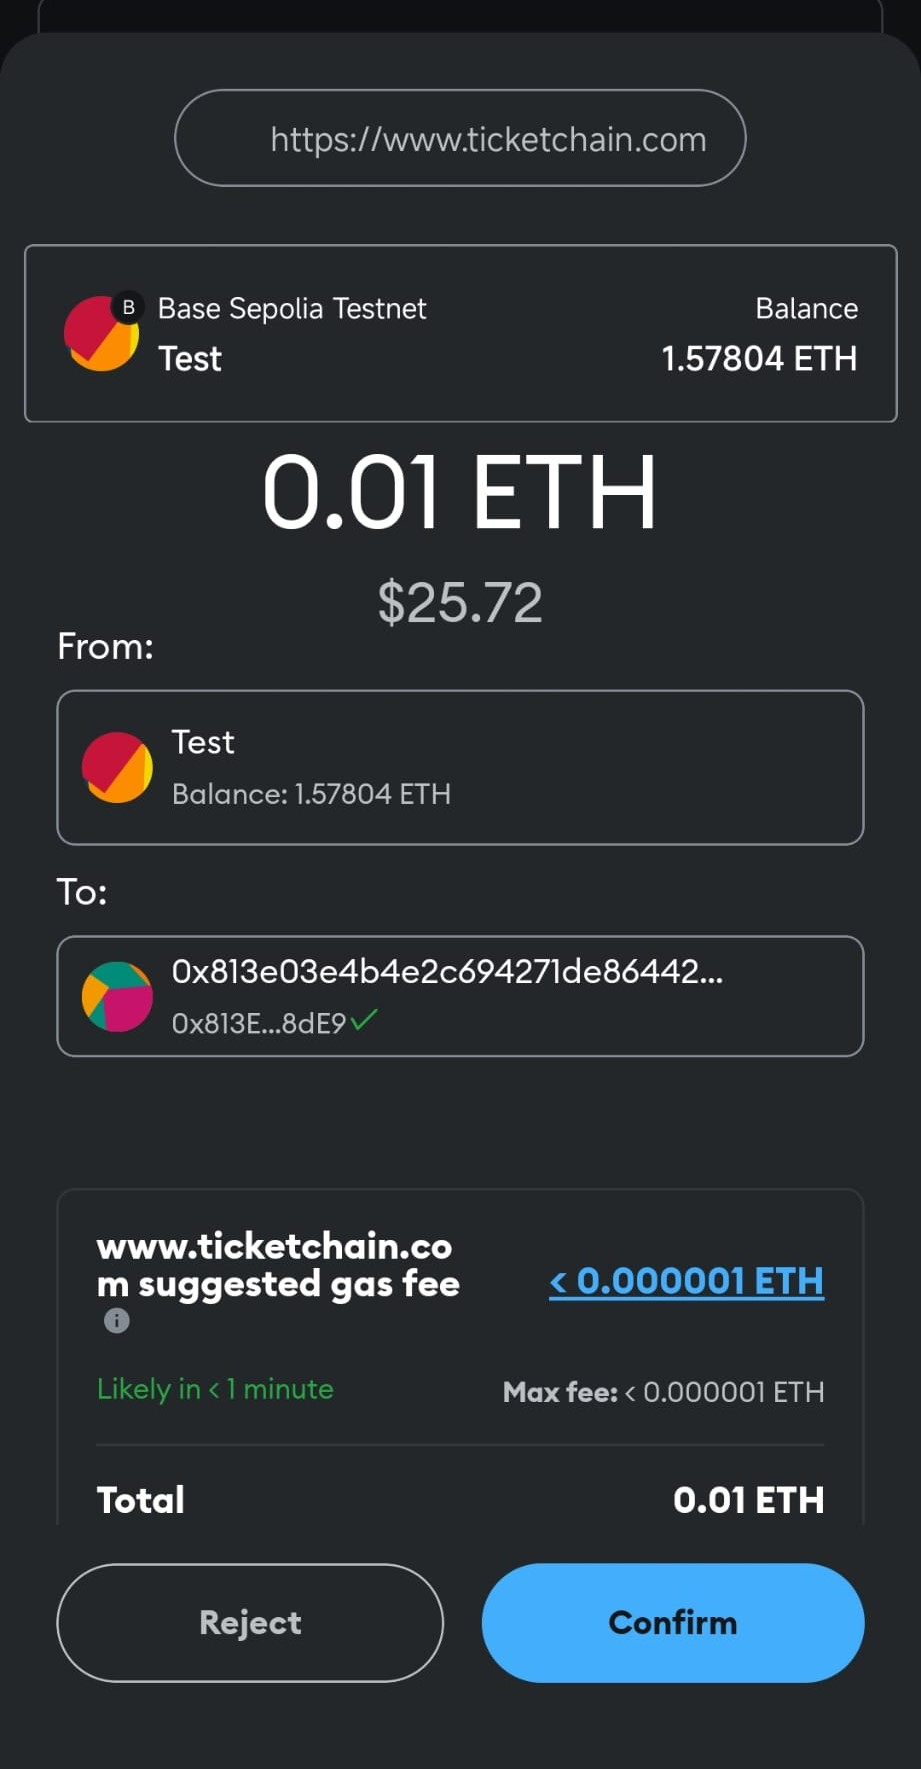
\includegraphics[width=\textwidth/3,frame]{MetaMask transaction prompt.jpg}
	\centering
	\caption{MetaMask transaction prompt}
	\label{fig:metamask_transaction_prompt}
\end{figure}

\subsection{Tickets}
\label{subsec:tickets}

After confirmation, the user is redirected back to the app, where he will be
able to see the events which he owns any tickets, on the profile page, the
second tab with the profile icon, along with the button to disconnect from the
wallet, like shown in the Figure \ref{fig:profile_page}.

\begin{figure}[H]
	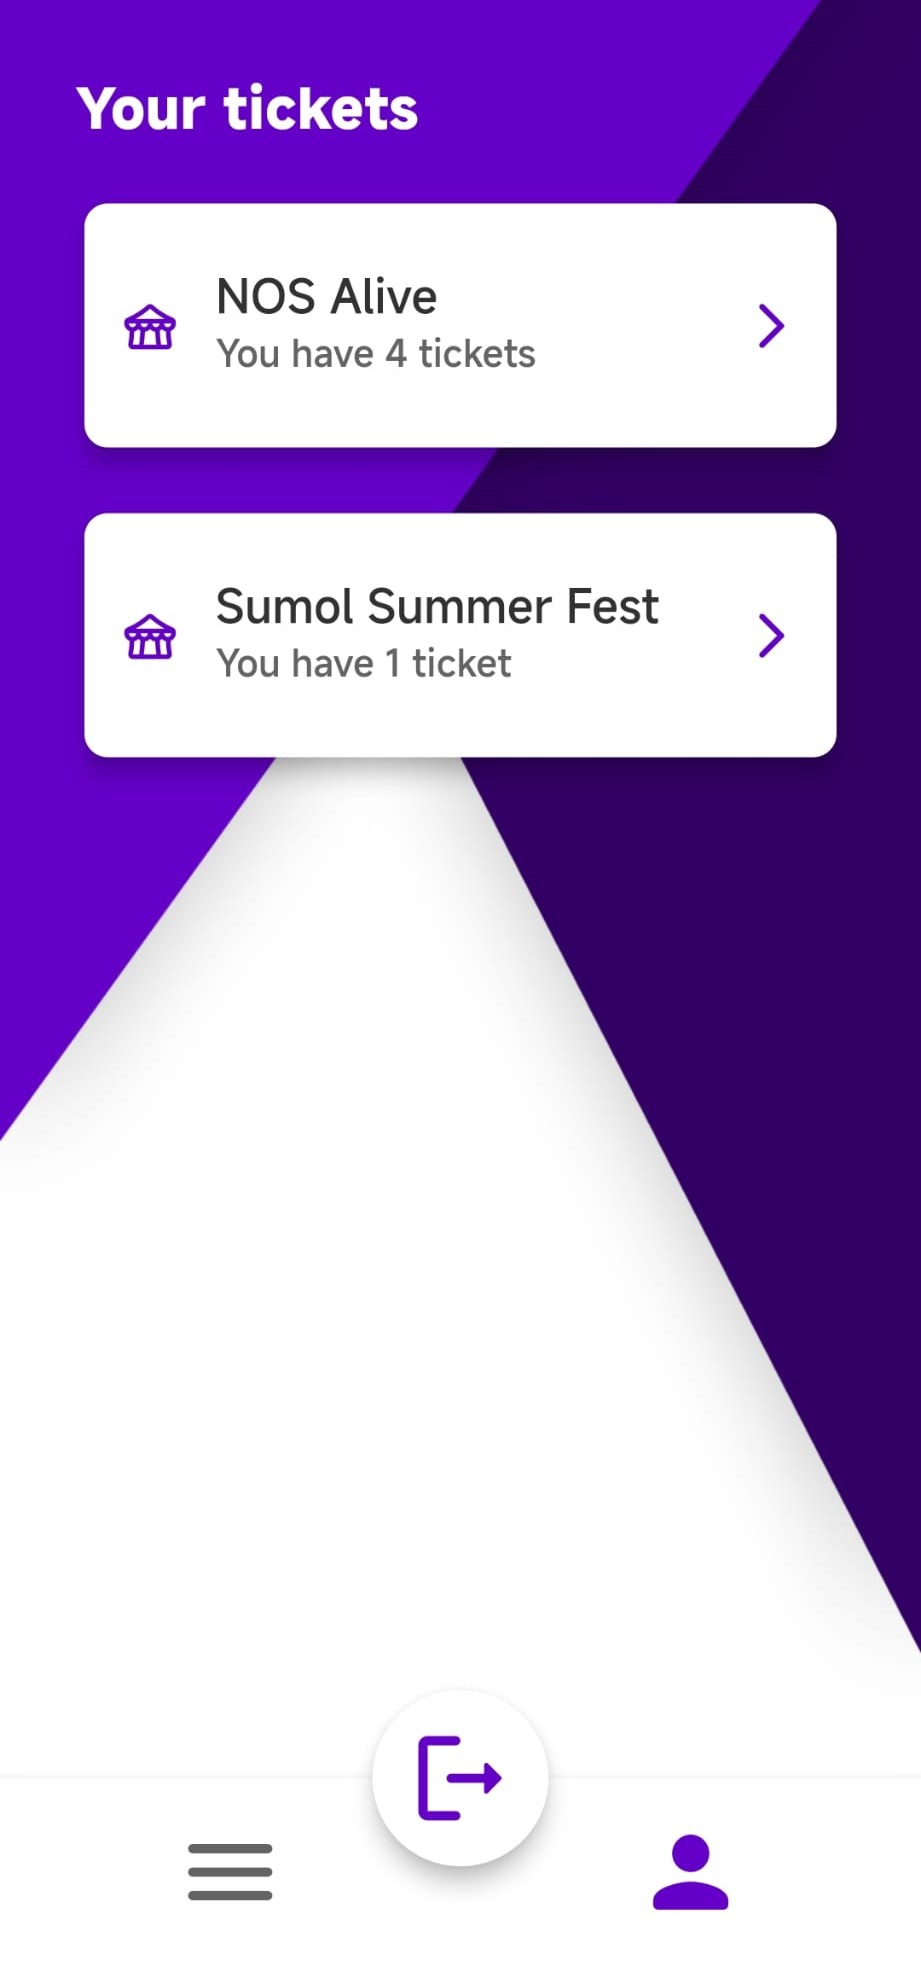
\includegraphics[width=\textwidth/3,frame]{Profile page.jpg}
	\centering
	\caption{Profile page}
	\label{fig:profile_page}
\end{figure}

Going into one of them, like the Figure \ref{fig:tickets_page} shows, the user
can see the tickets he owns for that event. It's a similar page as the normal
event one, but with the tickets he owns instead of the packages available. We
see 4 tickets here and the first one has a mark on it. This means the ticket
has already been validated. In the real world, a user do this doesn't make
sense, but we did it to make sure we handle every case.

\begin{figure}[H]
	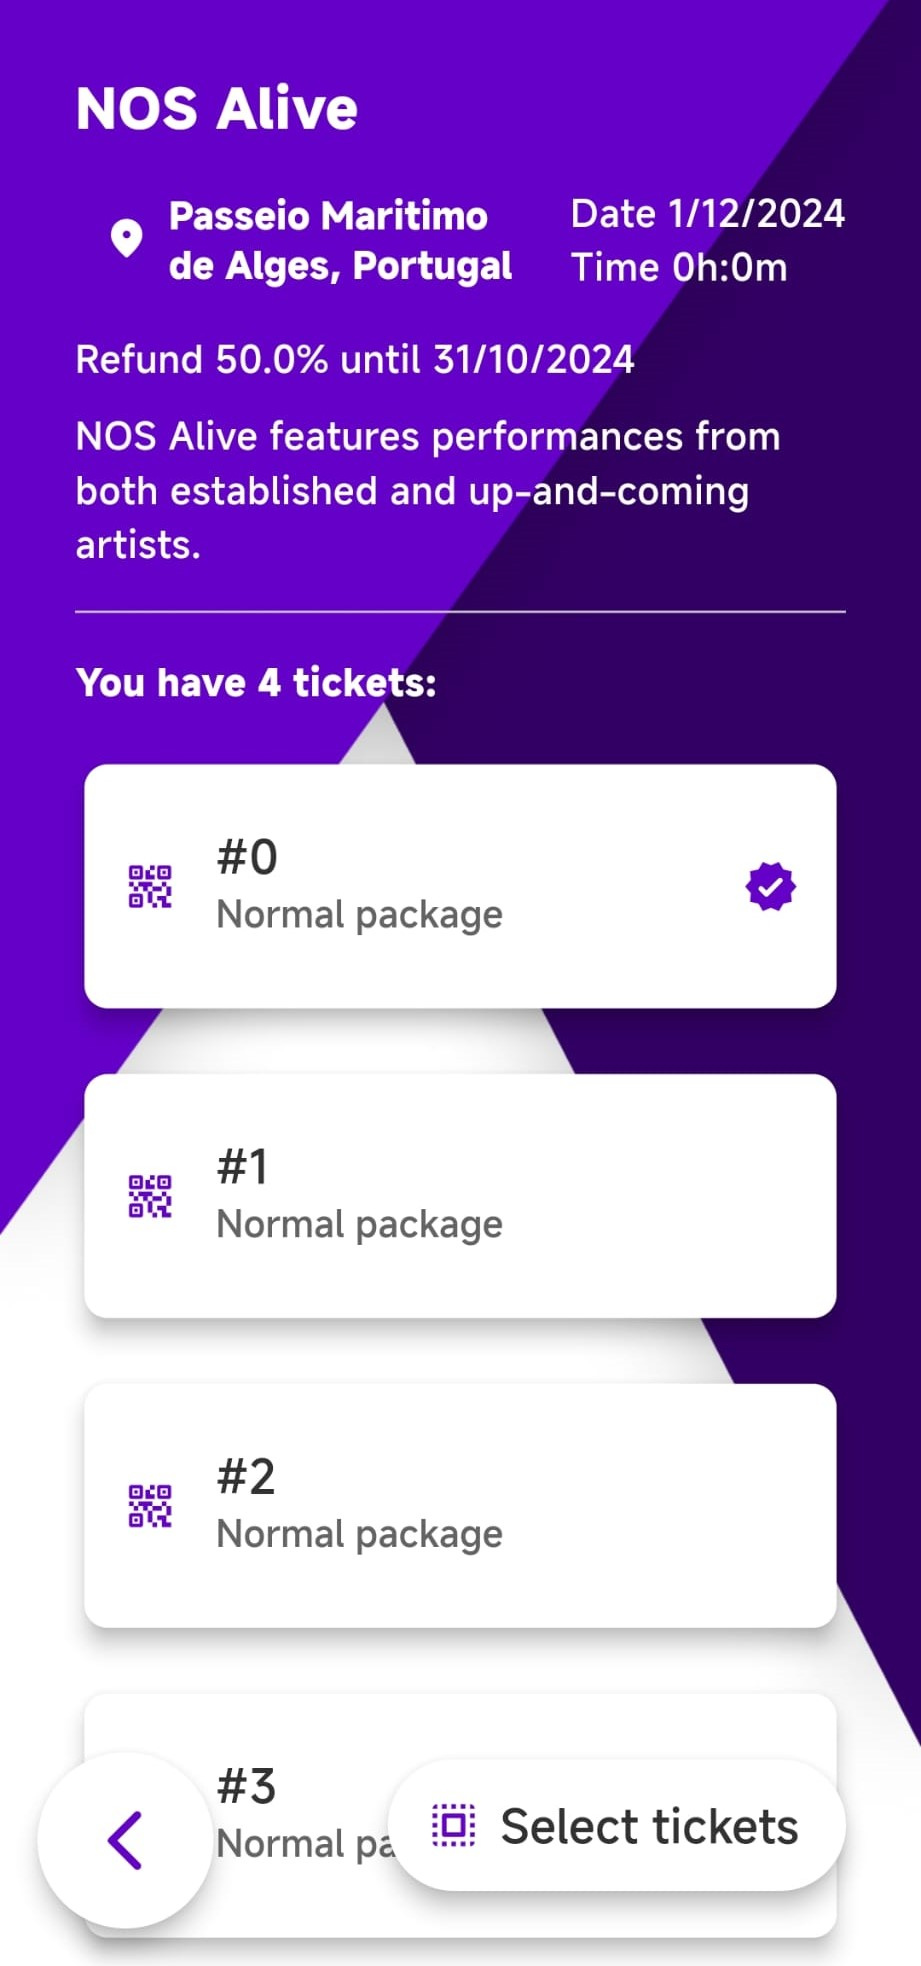
\includegraphics[width=\textwidth/3,frame]{Tickets page.jpg}
	\centering
	\caption{Tickets page}
	\label{fig:tickets_page}
\end{figure}

Clicking on one of the tickets, it shows us the basic ticket information, along
with its image, like shown in the Figure \ref{fig:ticket_information}.

\begin{figure}[H]
	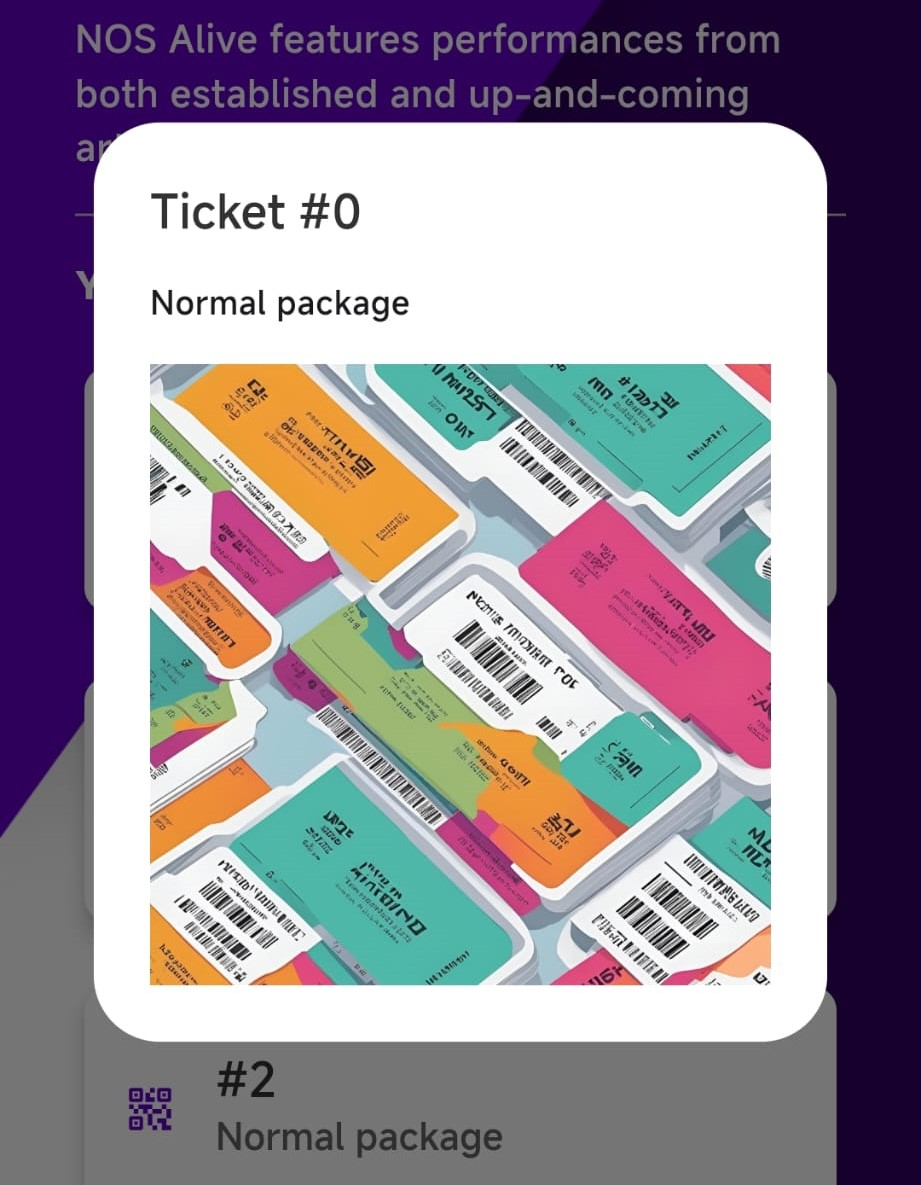
\includegraphics[width=\textwidth/3,frame]{Ticket information.jpg}
	\centering
	\caption{Ticket information}
	\label{fig:ticket_information}
\end{figure}

For operating the tickets, the user can simply click on the select tickets
button which will allow him to choose the tickets which he wishes to operate,
like shown in the Figure \ref{fig:ticket_operations}. In this case the user
sees only 3 tickets (while the Figure \ref{fig:tickets_page} shows 4) because
since the first is already validated, it's not possible to operate on it
anymore. We see the options to gift, refund and validate the tickets he
selected.

\begin{figure}[H]
	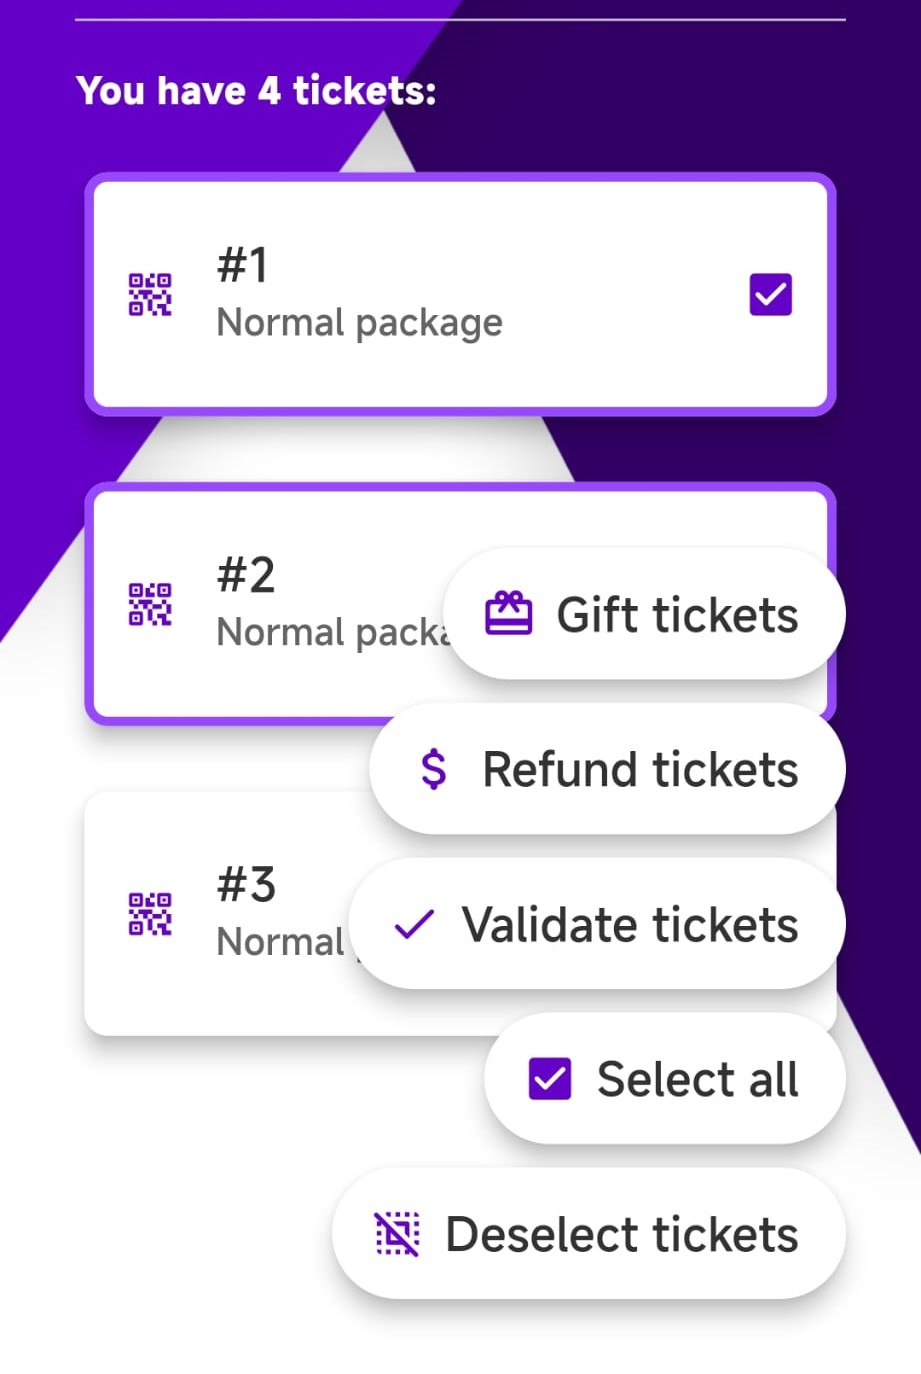
\includegraphics[width=\textwidth/3,frame]{Ticket operations.jpg}
	\centering
	\caption{Ticket operations}
	\label{fig:ticket_operations}
\end{figure}

The gift option will ask the user for the address to which he wants to gift the
tickets. After that, it will trigger the wallet to sign the transaction, and
the tickets will be transferred to the address.

The refund option will ask the user to confirm the refund, and trigger the
wallet to confirm the transaction in which the tickets will be burned, making
them available again for other users to buy, and returning the correct amount
of money to the user.

The validate option will start the validation process, which will be explained
in the Section TODO.

% 
% 

\section{TODO Validator App}
\label{sec:validator_app}

For the validator app, we will have a simple interface for the validators to
execute the process mentioned in the Figure \ref{fig:ticket_validation}.

[TODO mention the wallet being local]

%  The app itself will behave as a wallet in this case, to make things simple. 
% So basically the app will generate a private key and when the validator validates the tickets, the app will sign the message with the private key and send it to the blockchain. Since this is done by our system, when the validator has the app, the organizer will need to pass him some funds

Since the validators need to sign the message, the organizer just has to make
sure the validators have enough funds to pay for the transaction.

\subsection{Ticket Validation}
\label{subsec:ticket_validation}

For the ticket validation, we must take into consideration a lot of aspects,
because it's not just checking if the user address has a ticket associated to
him. This is because, since the data is on the blockchain, anyone can see the
addresses where each ticket belongs to, and pretend he's the owner of the
ticket. For this to be secure, we need to guarantee the user is actually the
owner of the address, and here is where the cryptographic message signature
comes in, the same process that happens when executing a normal blockchain
transaction.

We came up with the process shown in the Figure \ref{fig:ticket_validation},
that shows the steps between the actors and the system to validate the tickets.

\begin{figure}[H]
	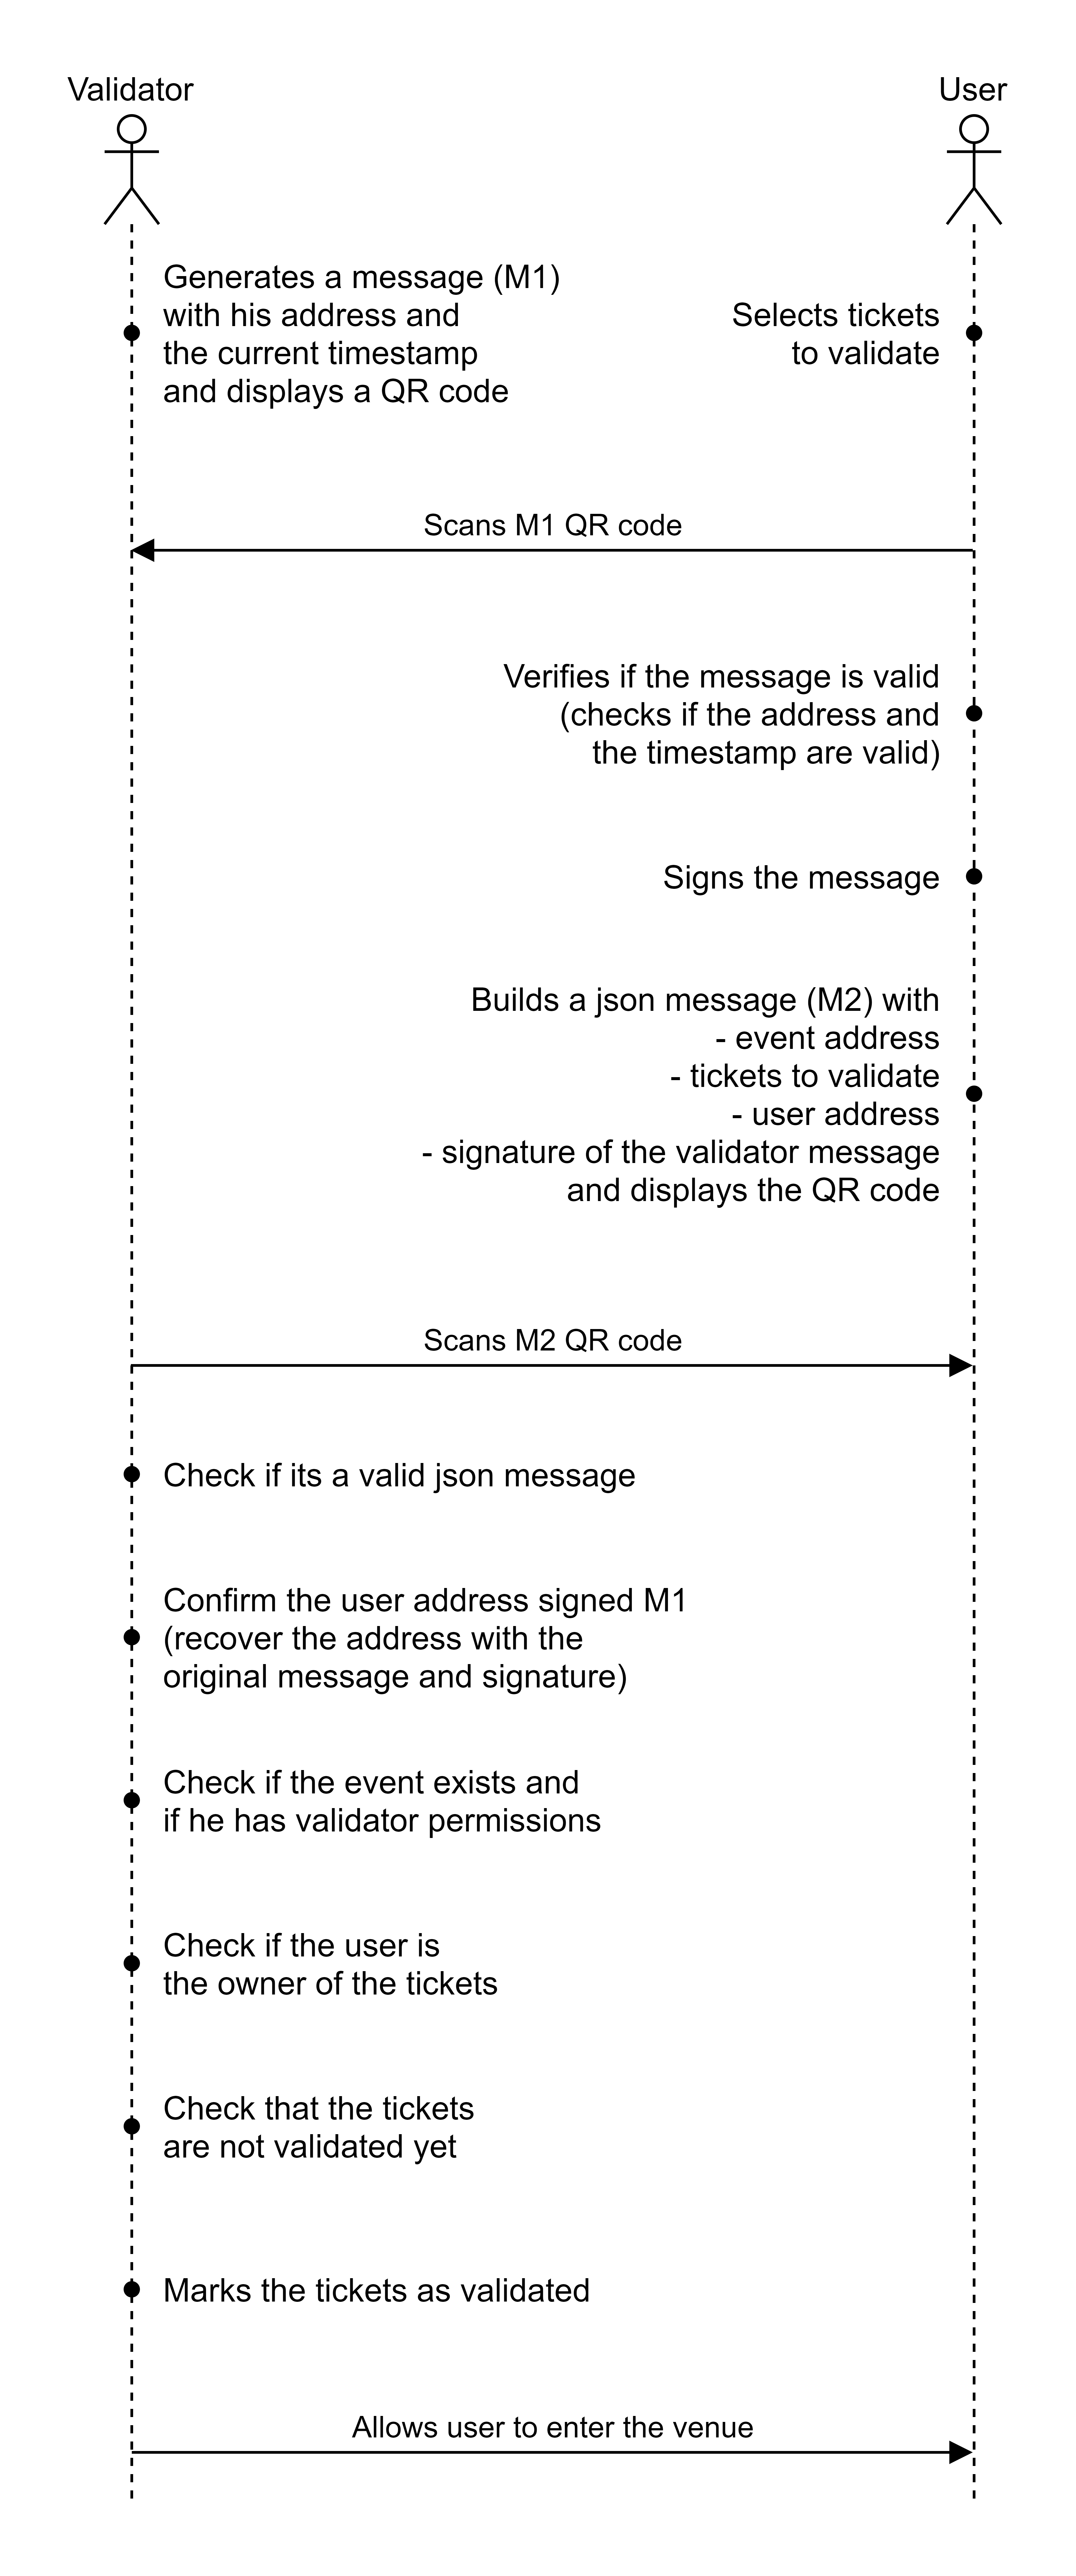
\includegraphics[width=\textwidth*2/3]{Ticket validation.png}
	\centering
	\caption{Ticket validation}
	\label{fig:ticket_validation}
\end{figure}

Here we see that the user reads the QR with a generated message from the
validator, signs it with his wallet, and generates a JSON with the signature
and useful information like the tickets to validate, the event, and the user
address. After the validator reads the JSON in the QR code, he checks if the
parameters match the ones on the blockchain, gets the address using a
cryptographic method to recover it through the original message and it's
signature, and checks if the user is the owner of the tickets. If everything
matches, the validator will trigger a transaction to mark the tickets as
validated, to avoid people sharing the accounts and using the same ticket
multiple times.

Both parties need to know the original message, so it matches. We could just
use a default message for everyone, so the users would just need to give the
signature to the validator, but this could become a security issue in case the
signature gets leaked, because anyone who has it could pretend to be a
different address. The idea here is to have a unique message for each user at
the time of the event, so it forces the user to sign it.

All this is reduced to a single transaction on the blockchain because,
depending on the network, the finality of a transaction (the time it takes for
a transaction to be fully registered on the blockchain) can take a while. This
was planned to be done in a single transaction to avoid congestion at the
entrance of the venue, so the users can enter the event with the least amount
of delay. This is an important aspect to consider when designing the system to
fullfil the system being fast, so like mentioned in the Section
\ref{subsec:non_functional_requirements}, the network choice is crucial.

\section{Main Smart Contract}
\label{sec:main_smart_contract}

The deployment will be done using \href{https://book.getfoundry.sh/}{Foundry},
a toolkit for the development and deployment of the smart contracts, which
makes it easy to deploy to any network, and also to test the contracts locally.

So smart contracts are similar to C++ mainly because it lies on a class-like
structure with variables to store data and methods, where the main difference
is that a class is called a contract and you can extend others to integrate
their functionalities. That's essentially what's gonna happen with each event,
extending the ERC721 standard, making it a collection of NFTs, where each NFT
is a ticket. Since this is the behavior we want (each event being a NFT
collection), we will have to deploy (instantiate, in C++) a new contract for
each event, so we will have a main contract to keep track of these events.

With this in mind, we created the Ticketchain main smart contract UML, like the
Figure \ref{fig:system_uml} shows. This contract will track the organizers and
the events associated with the system, along with the method to register a new
event with the necessary data, restricted to only organizers (to avoid
unauthorized people to interact).

\begin{figure}[H]
	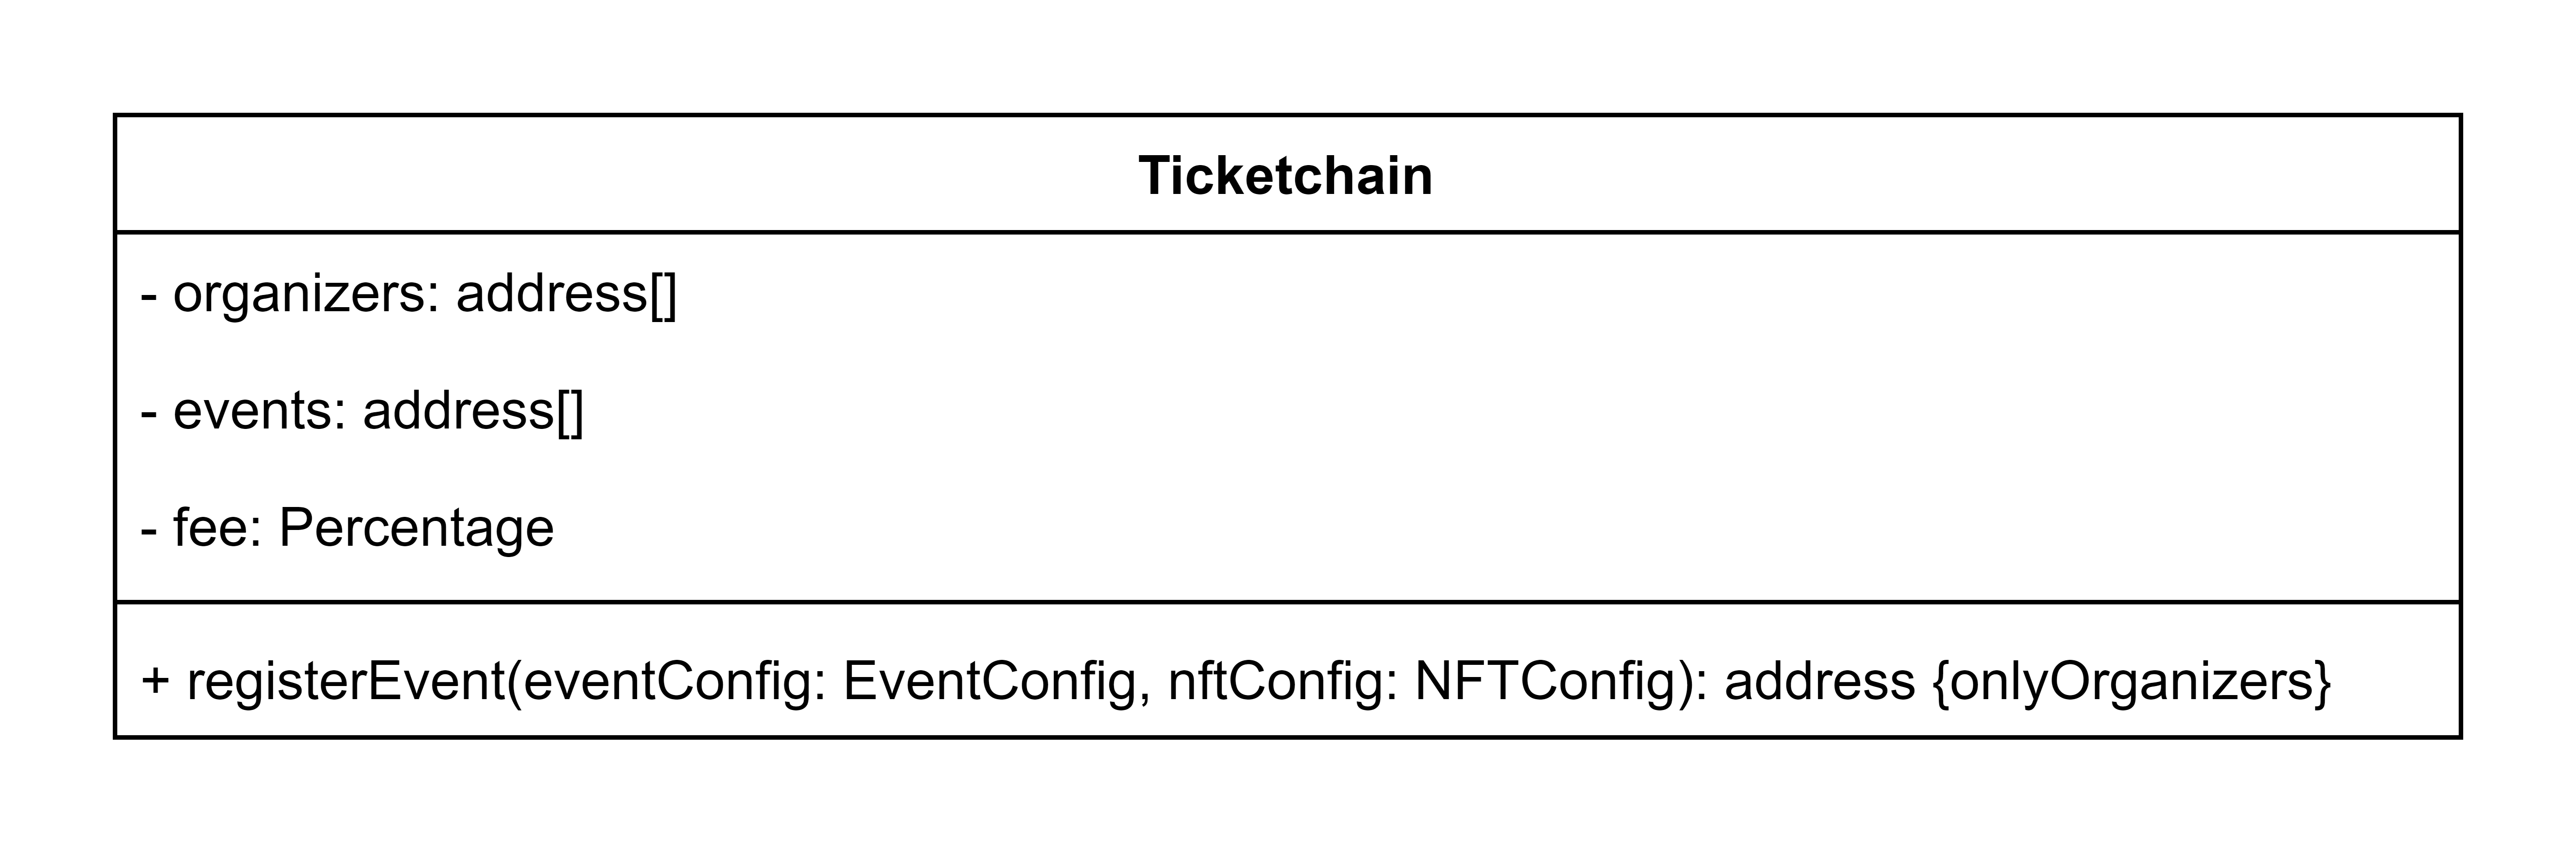
\includegraphics[width=\textwidth]{Ticketchain UML.png}
	\centering
	\caption{Main smart contract UML (simplified)}
	\label{fig:system_uml}
\end{figure}

With this structure, since we have this main contract where all the events of
the system are stored, we can simply make a call to get them all, showcasing
them in the app's home page for users to search. Any event that is deployed
outside the system or if it gets removed from there, it won't be shown to the
users.

\section{Event Smart Contract}
\label{sec:event_smart_contract}

For the event contract, we'll be extending the ERC721 standard and adding the
necessary methods to interact with the tickets, like buying, selling, and
validating them. The reason to extend this standard and not implement the logic
manually is because it makes it compatible with the most common marketplaces
for NFTs, which allows for users to do what they desire with them after the
event. It also has the necessary methods to manage the tickets, like
transferring them between users, and the necessary operations to track these
operations.

\subsection{ERC721 Structure}
\label{subsec:erc721_structure}

The standard was obtained through the
\href{https://docs.openzeppelin.com/contracts/api/token/erc721#ERC721}{OpenZeppelin}
library, which is a collection of secure and community-vetted smart contracts
that are used by many projects in the Ethereum ecosystem. This library is a
great resource for developers to build secure and reliable smart contracts.

Analyzing its source code [TODO ref], and looking into the most important
variables and methods of the standard shown in the Figure \ref{fig:erc721_uml},
we can understand that the NFTs are simply a mapping of the token ID to the
owner address, so when you execute a transaction to get a token (this process
is called minting), the token ID is then associated to your address. Then for
each token it's possible set a URI, which is a link to the NFTs metadata,
usually being a JSON file with the necessary information about the token, like
the name, description, and image.

This link could point to anything, for example a google drive file, but the
common thing is to store the metadata on the IPFS, which is a decentralized
storage system, so the metadata is not stored on the blockchain itself
(onchain), which would be very expensive, but rather on a decentralized storage
system (offchain), which is much cheaper.

\begin{figure}[H]
	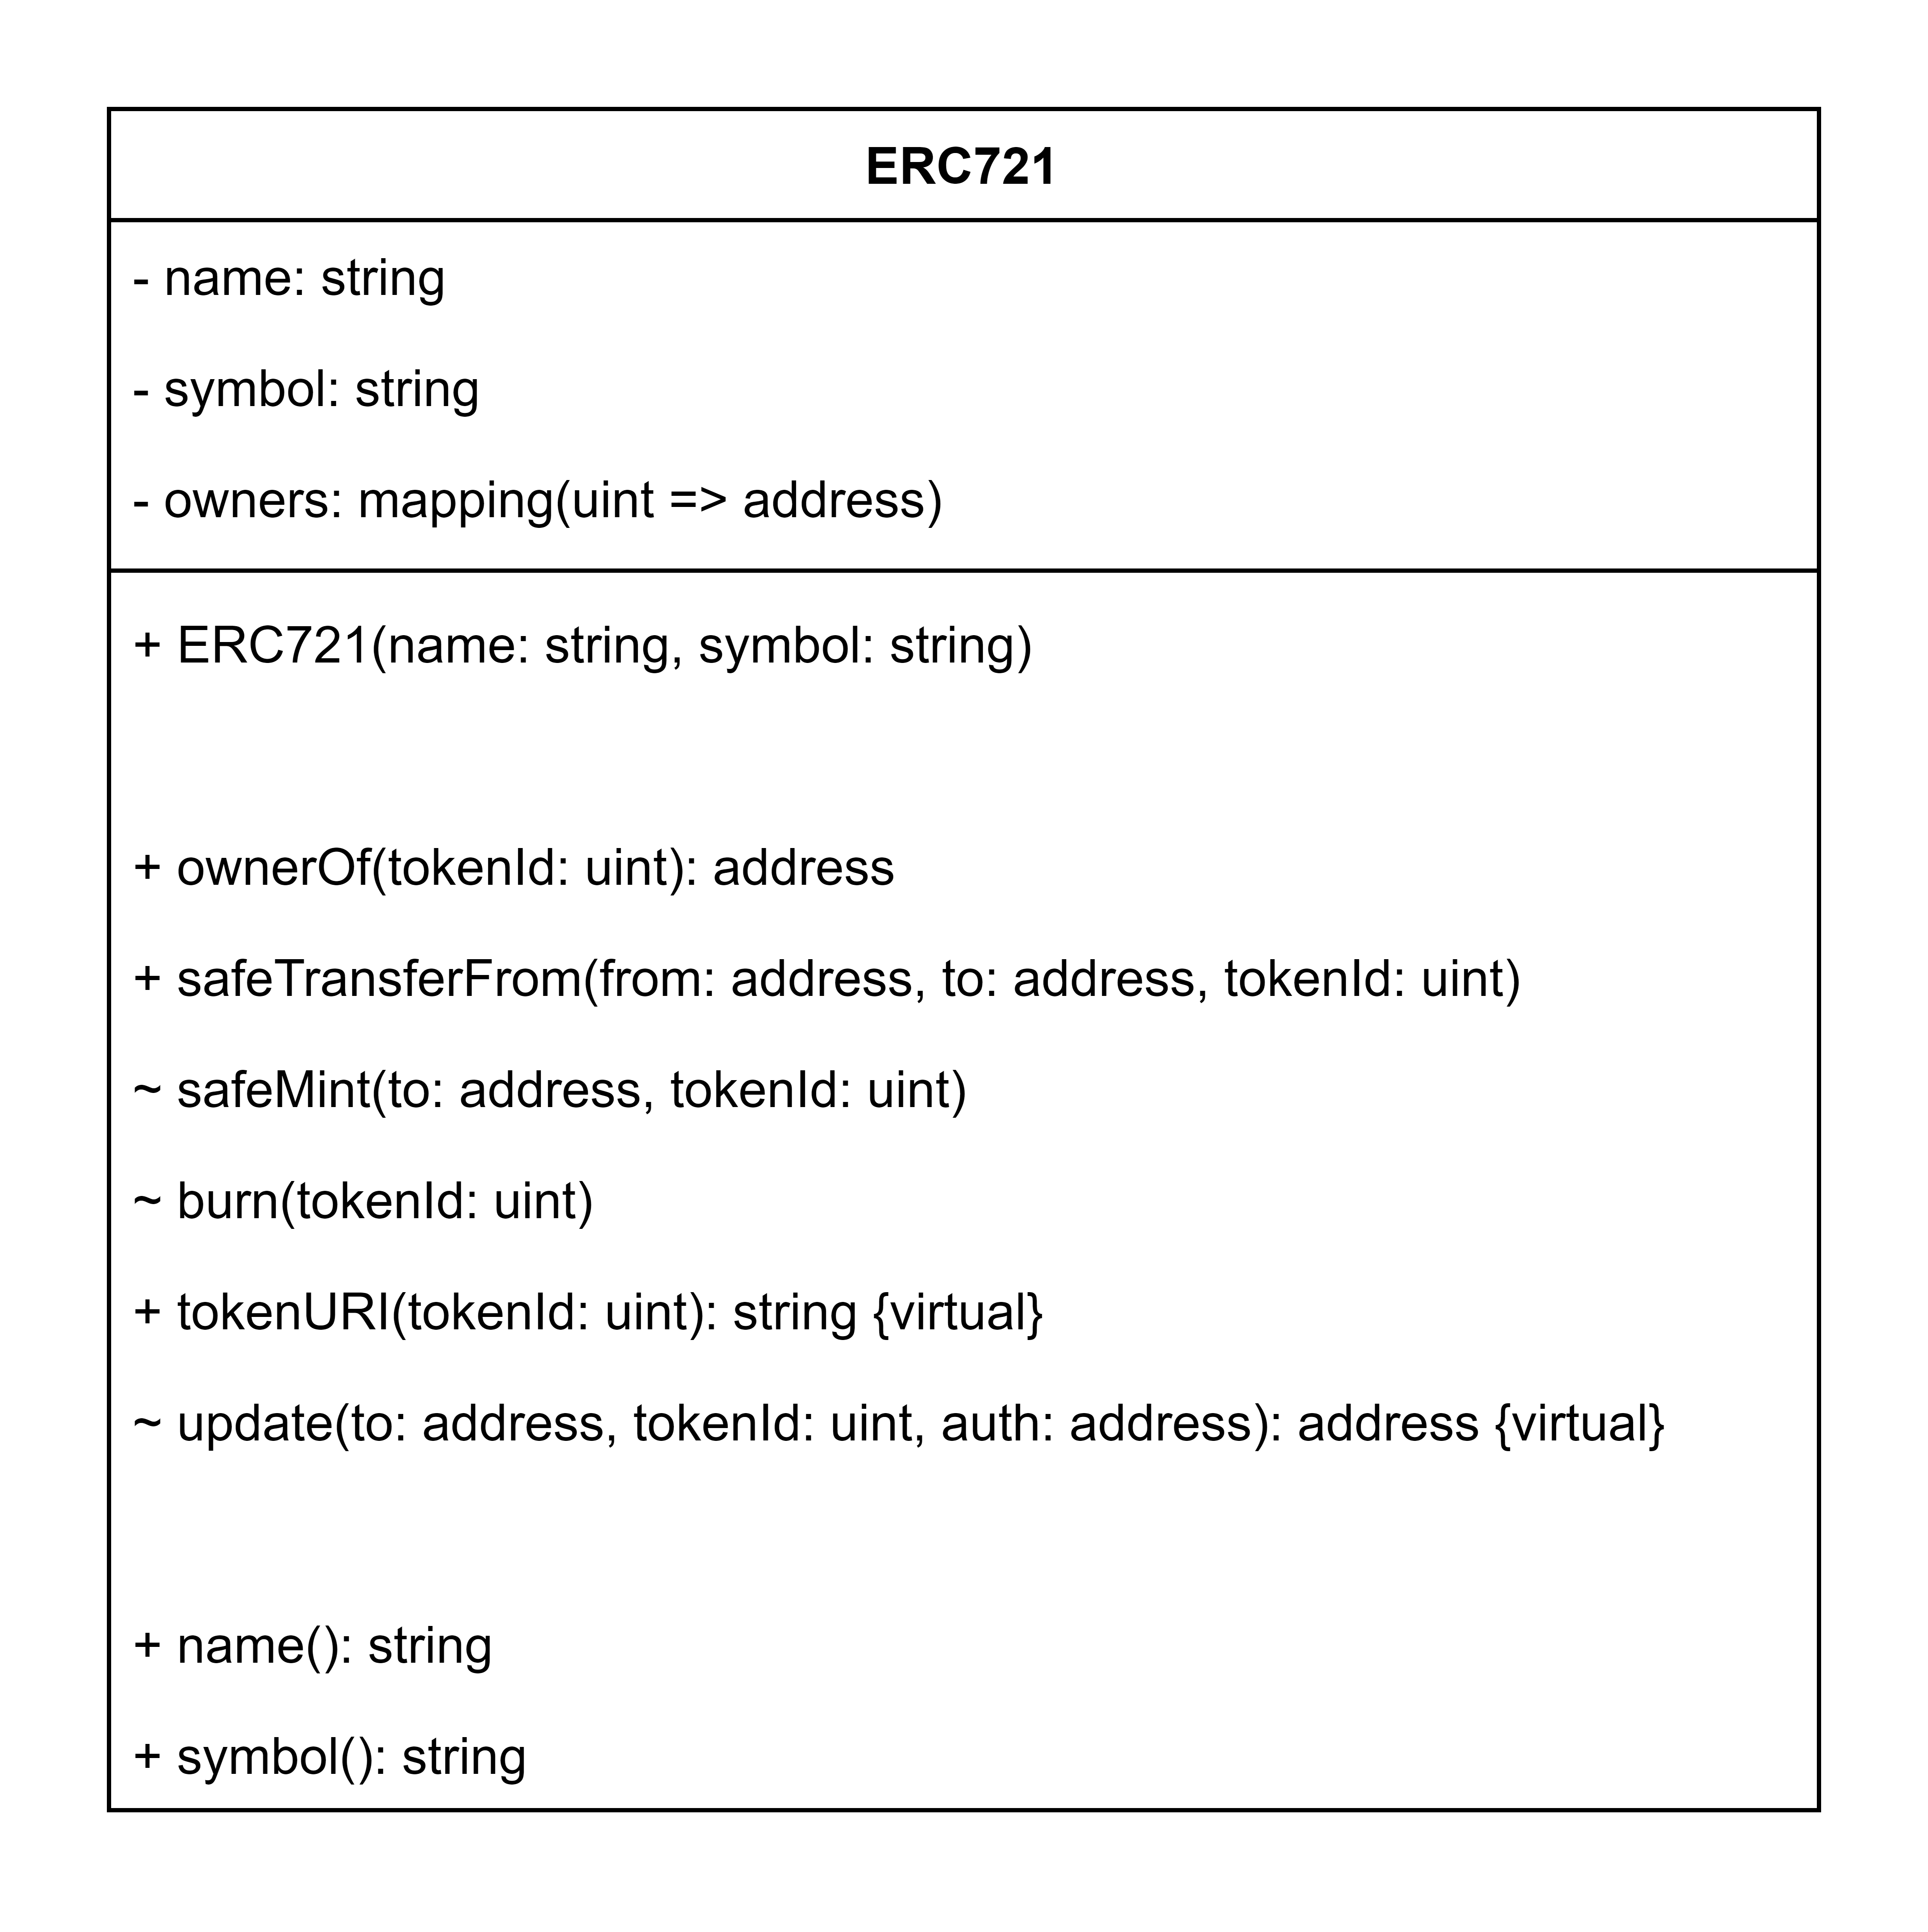
\includegraphics[width=\textwidth*2/3]{ERC721 UML.png}
	\centering
	\caption{ERC721 UML (simplified)}
	\label{fig:erc721_uml}
\end{figure}

The function \textit{tokenURI} is the one that is called by default in the
marketplaces to get the NFT's metadata, being one of the main reasons to extend
the ERC721 standard, because it enforces the implementation of this method. In
the Figure \ref{fig:erc721_uml} we see that it has the \textit{virtual}
keyword, meaning this can be overridden by the contracts that extend it, to
manipulate the way to store the metadata. We'll be mentioning this again in the
Section \ref{fig:package_logic}, about how the packages logic is implemented.

\subsection{Event Behavior}
\label{subsec:event_behavior}

So the event will be deployed and we need a certain control over the tickets.
One of the aspects we need to account for is that when deploying an event, and
since the event will extend the ERC721, any public functions on that standard
will be possible to execute. This is a problem because we don't want the users
to mint tickets whenever they want or transfer them between themselves from
outside the system, so we need to restrict these operations. As we saw already
on the Figure \ref{fig:erc721_uml}, only the \textit{safeTransferFrom} method
is public, so users could transfer NFTs between each other. We want that to be
possible, just not from outside the system, since that can lead users to
exploit the system and scalping the tickets easily. The minting, however, won't
be an issue because it's an internal method, so we will access it from the buy
method in the event and restrict it there.

The Figure \ref{fig:event_lifecycle} shows the lifecycle of the event, and what
restrictions are in place for the ticket operations. The dates above the line
indicate the states of the event, and below a small description of the
operations that are allowed when each state is reached.

\begin{figure}[H]
	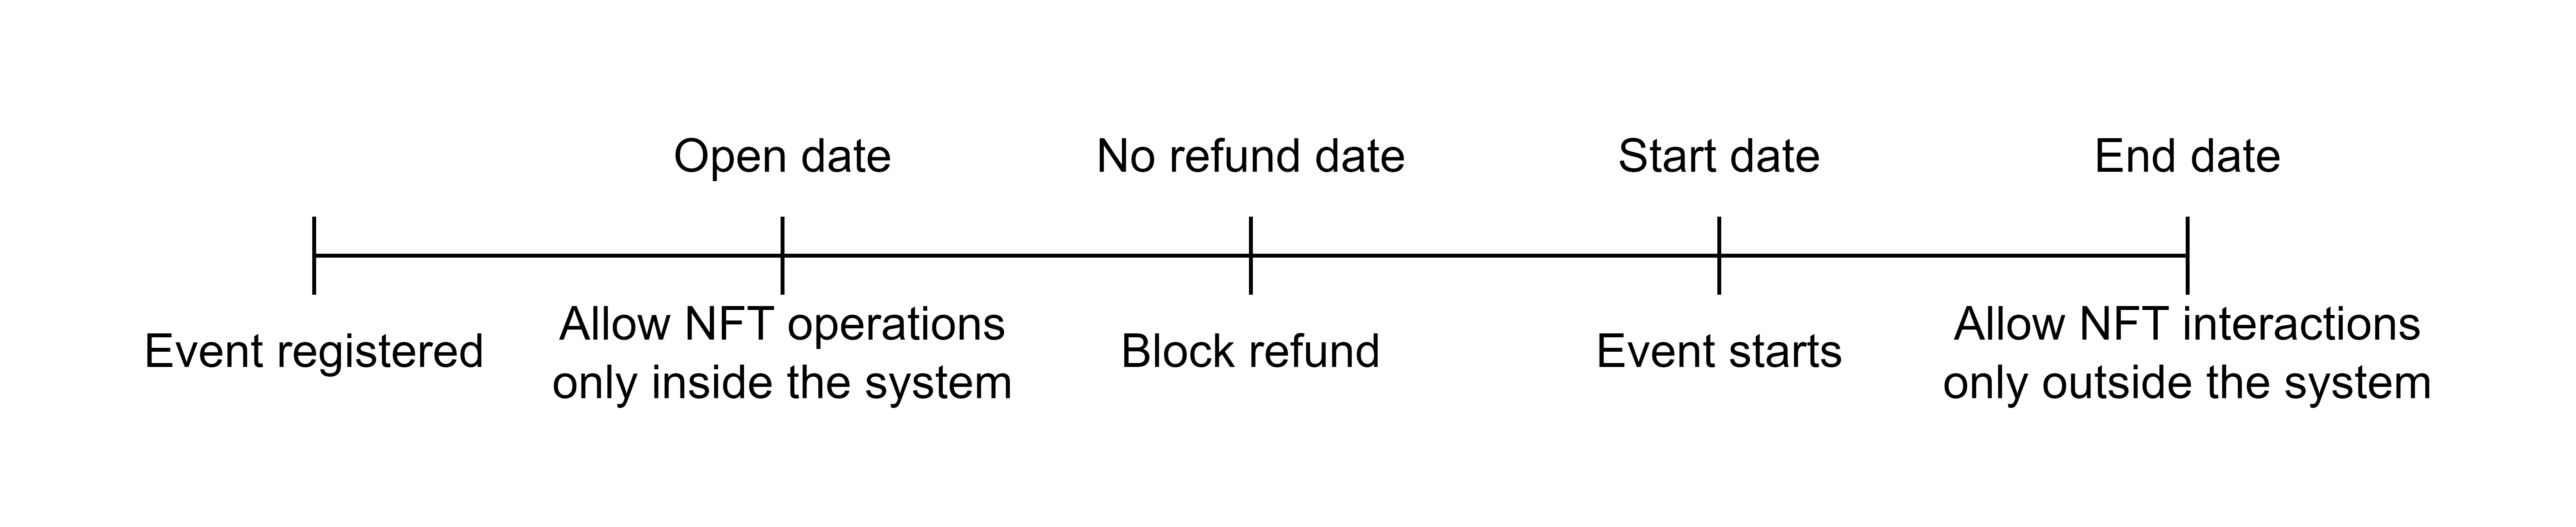
\includegraphics[width=\textwidth]{Event lifecycle.png}
	\centering
	\caption{Event lifecycle}
	\label{fig:event_lifecycle}
\end{figure}

We will have 4 main states for the event after it has been registered (the ones
in bold), being the \textit{Open}, \textit{No refund}, \textit{Start}, and
\textit{End} dates. Once the event is registered, it will show up in the app
for user to see, and the organizers can set a later open date to allow ticket
minting (buying).

\paragraph{Open Date:} Once it hits the \textit{Open} date, we will allow the users to buy tickets,
which will mint the NFTs by executing the \textit{safeMint} method of the
ERC721 contract. We will allow users to operate over the NFTs, but only within
the system. If they try to call the \textit{safeTransferFrom} directly from the
ERC721 standard, it will revert, because we detect it's not being called
through the system.

\paragraph{No Refund Date:} After the \textit{No refund} date, we will prevent the users to call the refund
method, which essentially \textit{burns} the NFTs, removing them from the user
and making them available again. This is a nice operation to add because it
allows the users to get their money back if they can't attend the event. The
organizer decides the percentage of the refund and the deadline, which is there
to prevent users to buy a big amount of tickets and then refund them last
minute, which would be a way to exploit the system (in case of a 100\% refund,
they wouldn't risk anything). The other good thing for the organizer is when
the event is expected to be sold out. Since the users will get some money back,
they will have a reason to refund their tickets if they cannot attend the event
anymore, making them available again for other users to buy at the original
price, making the organizer a higher profit. After this deadline, the only
that'll be allowed is for users to resell their tickets in the system's
marketplace, which them to sell at a higher price than the refund (but never
higher than the original, of course).

\paragraph{Start Date:} The \textit{Start} date is there to tell the users when the event starts, so
basically when the gates will open. That's the date that appears in the app, so
the users know when to show up.

\paragraph{End Date:} The \textit{End} date tells when the event is over, unlocking all the ticket
operations to outside the system. So users can simply keep the tickets as a
souvenir or sell them in any marketplace, without any restrictions on the
tickets, including the removal of the price cap.

With this behavior in mind, we came up with the Event UML, like shown in the
Figure \ref{fig:event_uml}, where we added the necessary methods for the
organizer/admins to manage the event and the users to handle the tickets, which
then trigger the corresponding methods of the ERC721 contract. We added a
possibility to have admins so the organizer can distribute the workload of
executing the necessary operations to people he trusts.

\begin{figure}[H]
	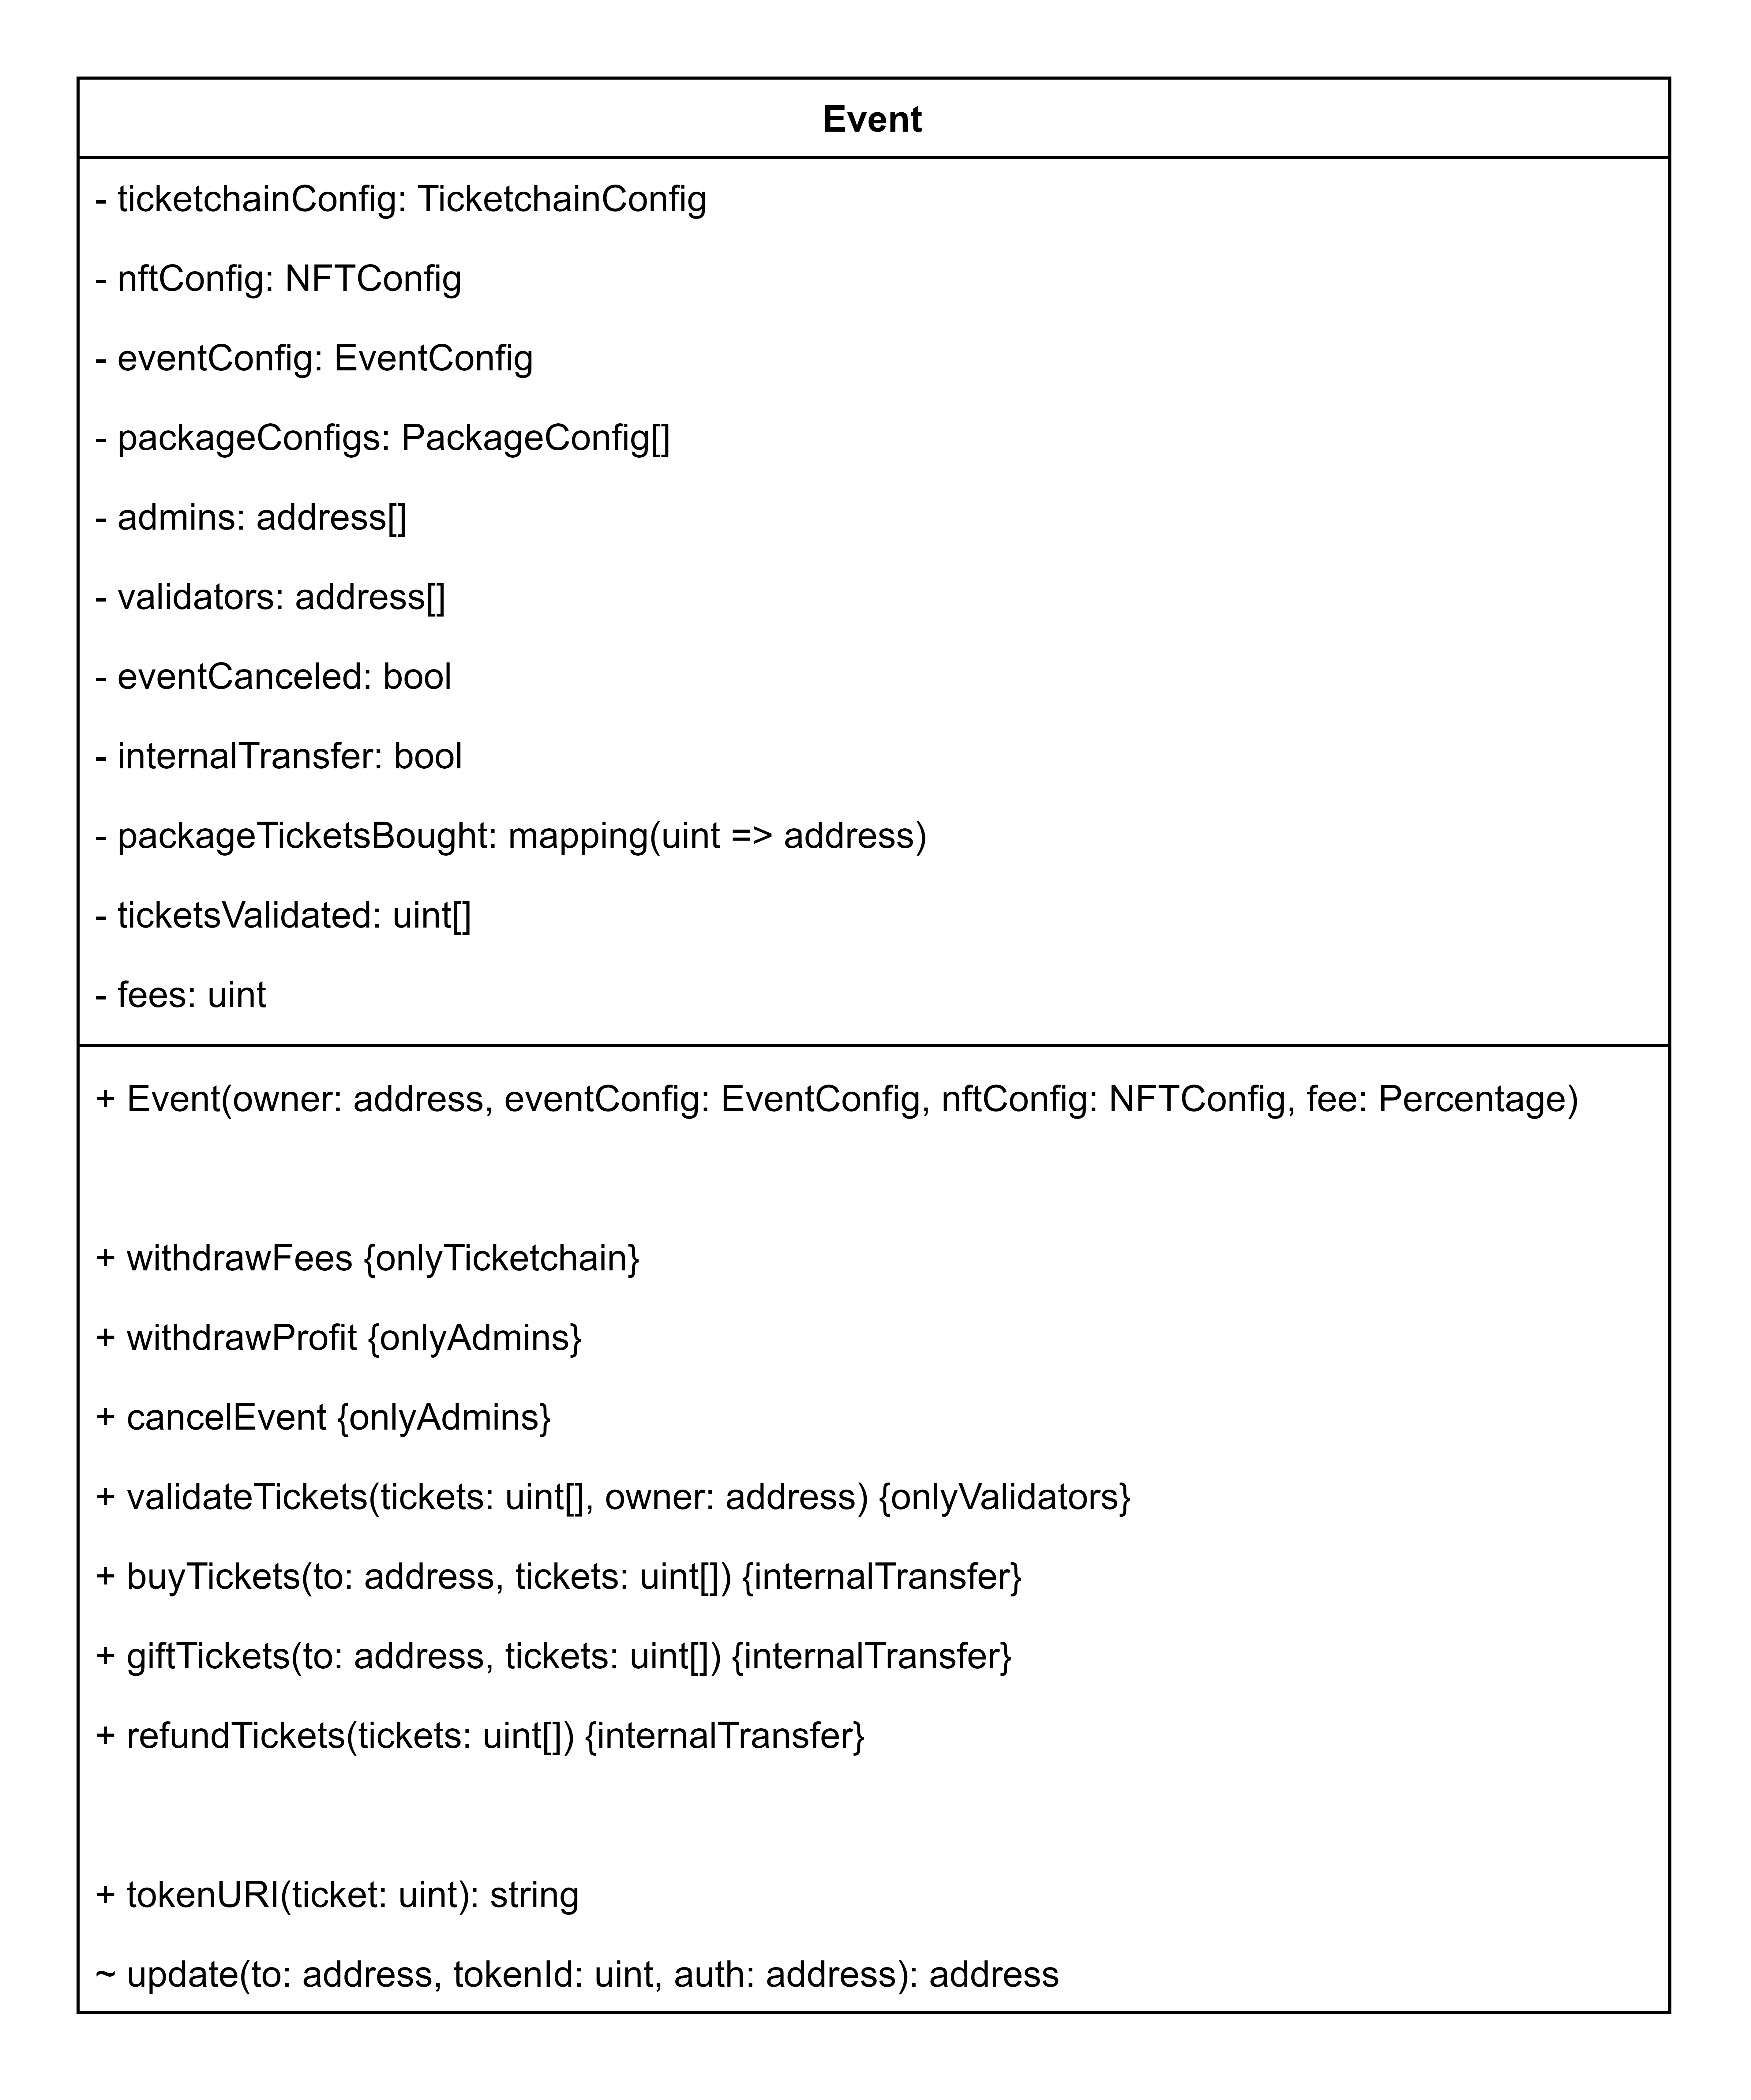
\includegraphics[width=\textwidth*3/4]{Event UML.png}
	\centering
	\caption{Event smart contract UML (simplified)}
	\label{fig:event_uml}
\end{figure}

As we can see, the \textit{update} method has been overridden from the ERC721
standard to restrict the interactions with the NFTs according the defined
behavior. This method is the one that gets called anytime there's an operation
on any NFT, so we can implement here the necessary logic to restrict the
operations, and we can visualize that in the following flowchart, shown in the
Figure \ref{fig:nft_flowchart}.

\begin{figure}[H]
	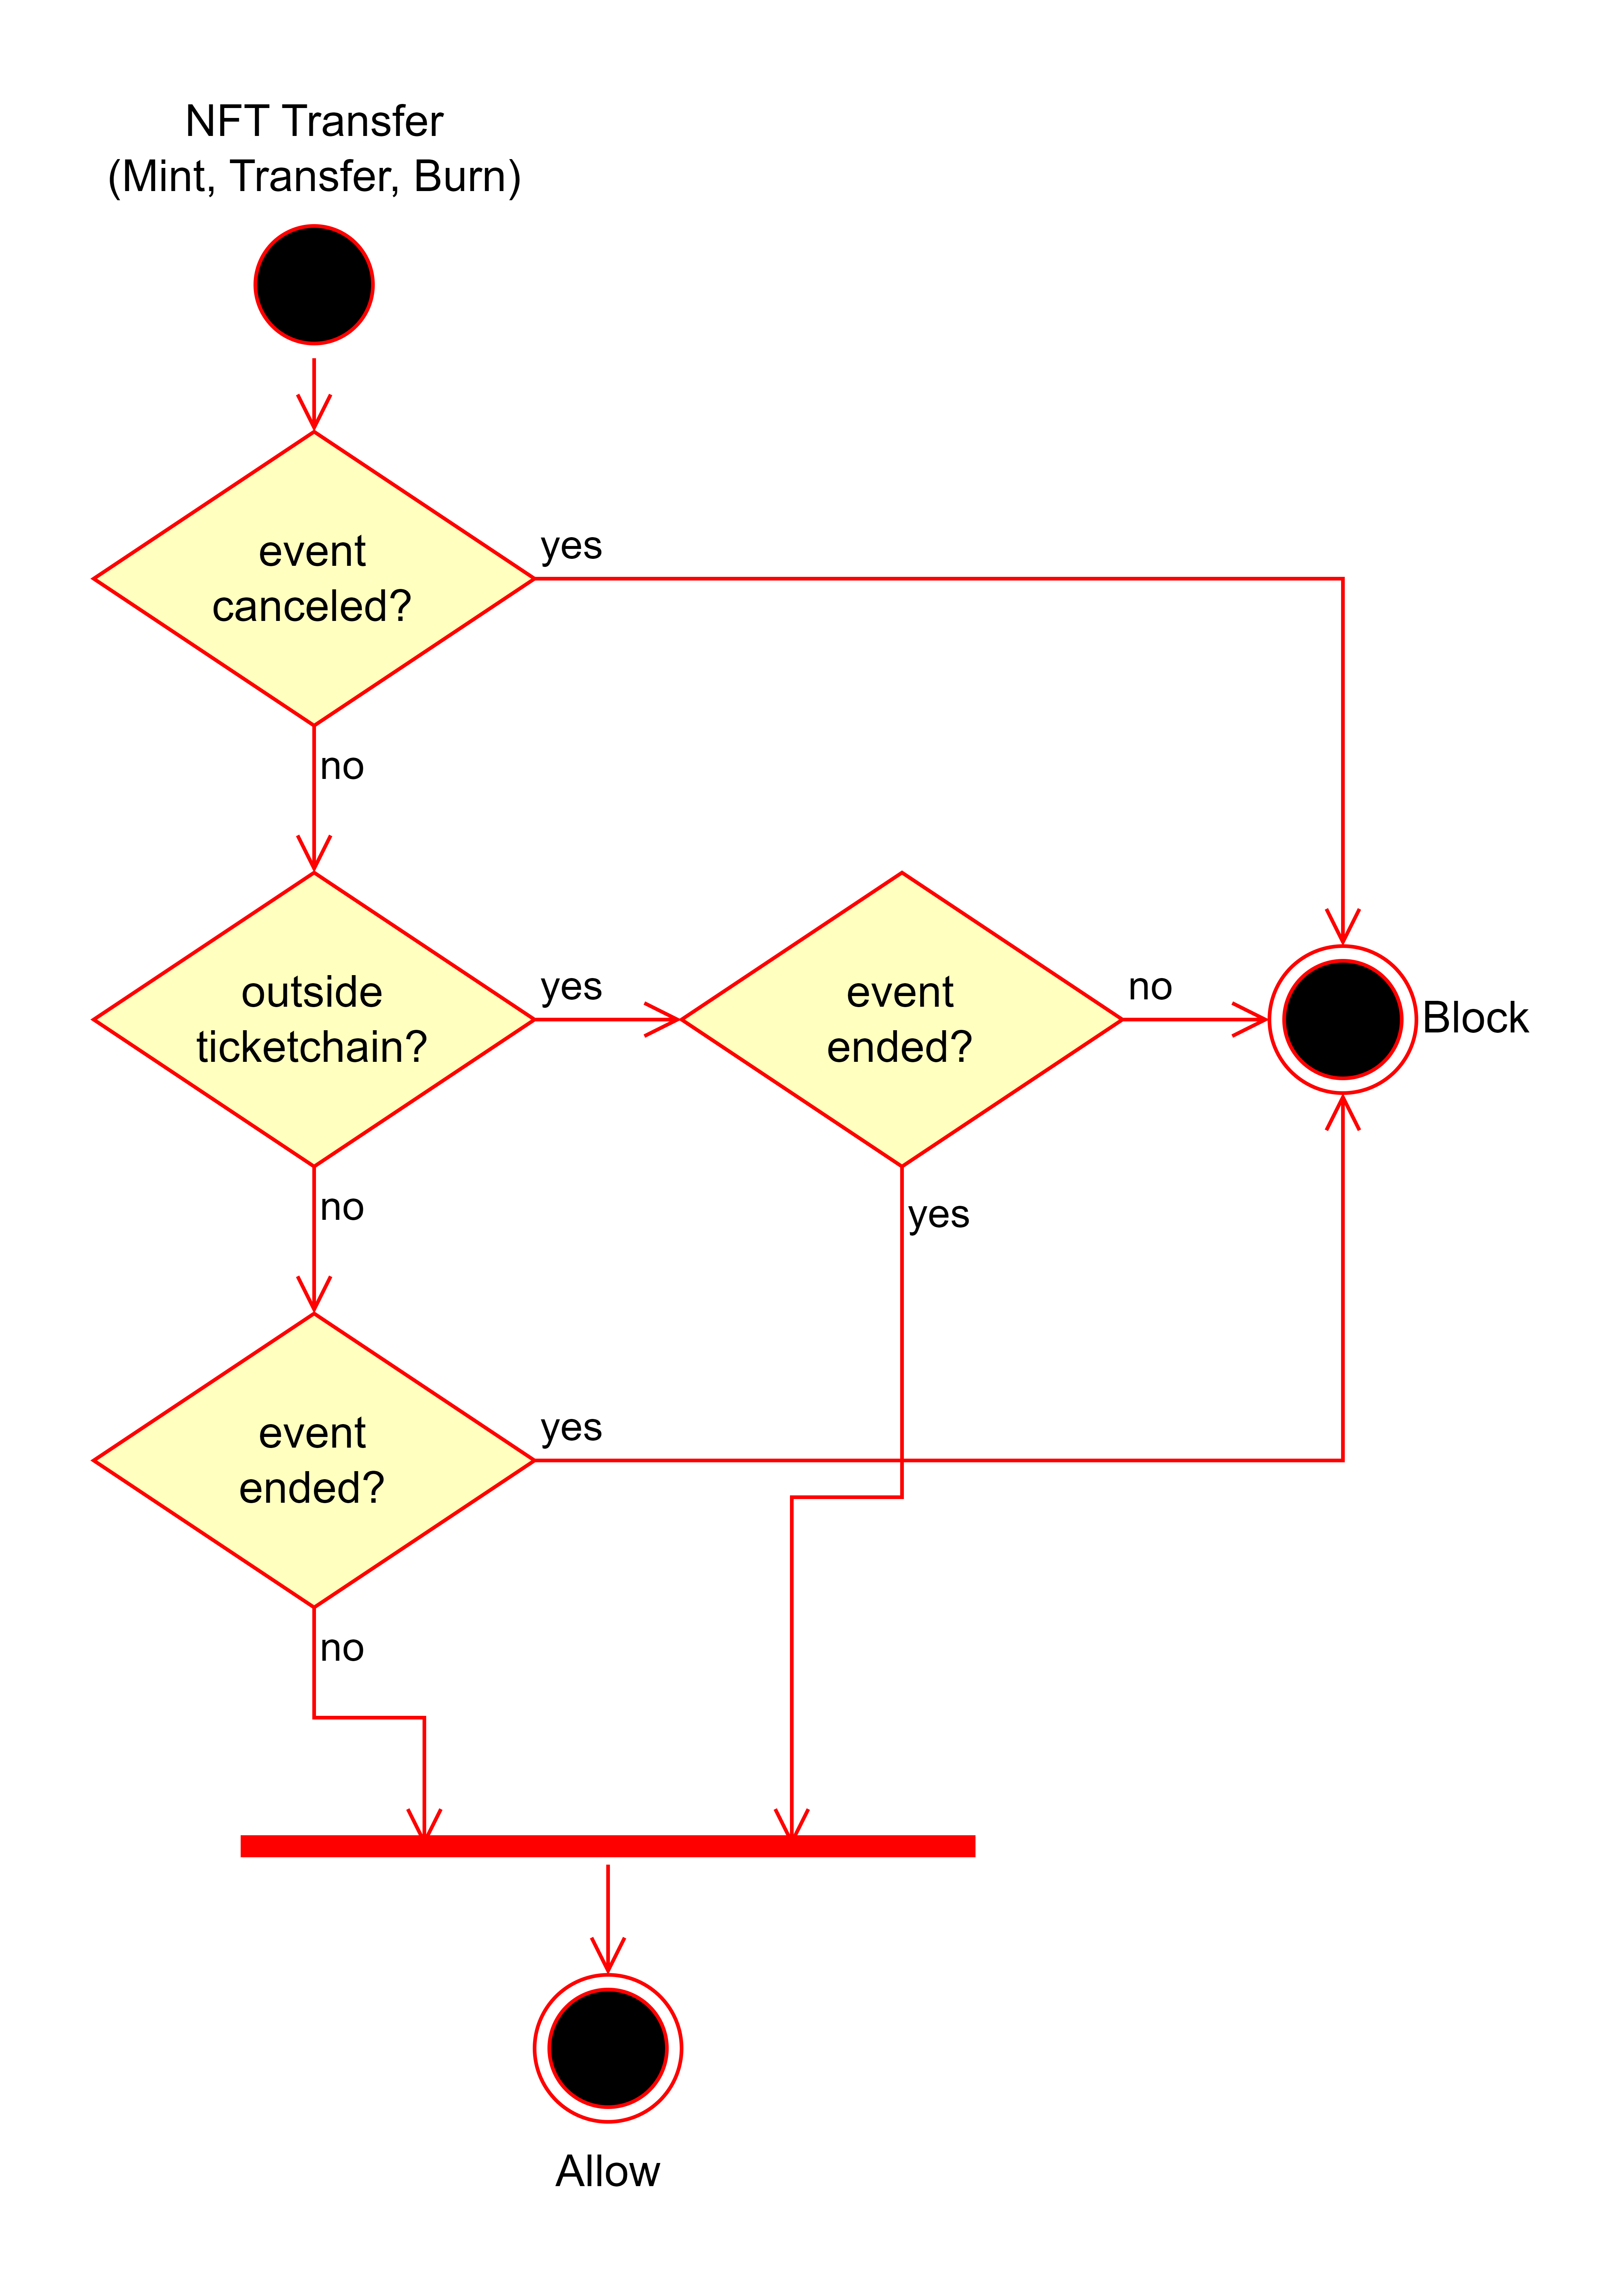
\includegraphics[width=\textwidth*2/3]{NFT flowchart.png}
	\centering
	\caption{NFT flowchart}
	\label{fig:nft_flowchart}
\end{figure}

This logic is possible to implement because of modifiers, mentioned before.
What we essentially do on that modifier, is set a variable to true (meaning the
NFT operation is coming from within the system), execute the function it's
assigned to, and then we set the variable back to false. Then we apply that
modifier on the necessary functions, which we can see them with the operator
	{internalTransfer} in the event UML, shown in the Figure
\ref{sec:event_smart_contract}.

\subsection{Structs}
\label{subsec:structs}

As is possible to see in the Figure \ref{fig:event_uml}, and also in the Figure
\ref{fig:system_uml}, we have a few custom structs to organize better the data.
These structs are the \textit{Percentage}, \textit{EventConfig},
\textit{NFTConfig}, \textit{PackageConfig} and \textit{TicketchainConfig}
structs.

\paragraph{Percentage Struct:} The \textit{Percentage} struct is necessary because in Solidity there are no
floating point numbers, so we need a way to make calculations with percentages.
What this struct does is it stores the value of the percentage and the amount
of decimals it has, so if we want to calculate 55.50\% of a number, we would
have 555 as the value with 1 decimal, or 5550 with 2 decimals.

The struct is as follows:
\begin{lstlisting}[caption=Percentage struct]
    struct Percentage {
        uint256 value;
        uint256 decimals;
    }
\end{lstlisting}
so to obtain a percentage of some $x$ number, we do $y = \frac{x \times
		\text{Percentage.value}}{100\mathrm{e}^\text{Percentage.decimals}}$.

When working with ether units, it can be common to have values like 0.00005
ether, but it's rather rare to have small values in wei, like 1000 wei, so
applying this formula won't lose much precision (note that 1 ether is $10^{18}$
wei).

\paragraph{TicketchainConfig Struct:} The \textit{TicketchainConfig} struct is simply to keep it stored the system
address and the system fee percentage, so we can easily access this information
when applying the fees and withdrawing them, and is as follows:
\begin{lstlisting}[caption=TicketchainConfig struct]
    struct TicketchainConfig {
        address ticketchainAddress;
        Percentage feePercentage;
    }
\end{lstlisting}

\paragraph{NFTConfig Struct:} The \textit{NFTConfig} struct is just to store the NFTs basic information, like
the name, symbol, and base URI, to ease the input of the NFTs information when
registering the event:
\begin{lstlisting}[caption=NFTConfig struct]
    struct NFTConfig {
        string name;
        string symbol;
        string baseURI;
    }
\end{lstlisting}
The is the name of the NFT collection and the symbol is the abbreviation of it,
like the name being 'Ticketchain' and the symbol being 'TCK', for example. The
base URI is the link to the metadata of the NFTs, which will be used to get the
information about the tickets.

\paragraph{EventConfig Struct:} The \textit{EventConfig} struct is to store the event's entire configuration,
like the name, description, location, dates, and refund, like this:
\begin{lstlisting}[caption=EventConfig struct]
    struct EventConfig {
        string name;
        string description;
        string location;
        uint256 openDate;
        uint256 noRefundDate;
        uint256 startDate;
        uint256 endDate;
        Percentage refundPercentage;
    }
\end{lstlisting}

\paragraph{PackageConfig Struct:} Lastly, the \textit{PackageConfig} struct is there to store each package
information, to keep track of the ones that are available for the event:
\begin{lstlisting}[caption=PackageConfig struct]
    struct PackageConfig {
        string name;
        string description;
        uint256 price;
        uint256 supply;
        bool individualNfts;
    }
\end{lstlisting}
This structure will be better discussed in the next Section
\ref{subsec:ticket_packages}.

\subsection{Ticket Packages}
\label{subsec:ticket_packages}

It's common to see events with different types of tickets, like VIP, standard,
or even 3-day passes, each with its own price and benefits. We want to
implement this feature in the system, so we can have a better control over the
tickets and the users can choose the one that fits them better.

For that, we will allow the organizer to add packages, indicating the supply of
each one, and as we saw already, the NFTs are a mapping of the ID to the owner,
so we can organize the packages as a list, where the supply and order of them
assigns the ID of each NFT to the package, like the Figure
\ref{fig:package_logic} illustrates.

\begin{figure}[H]
	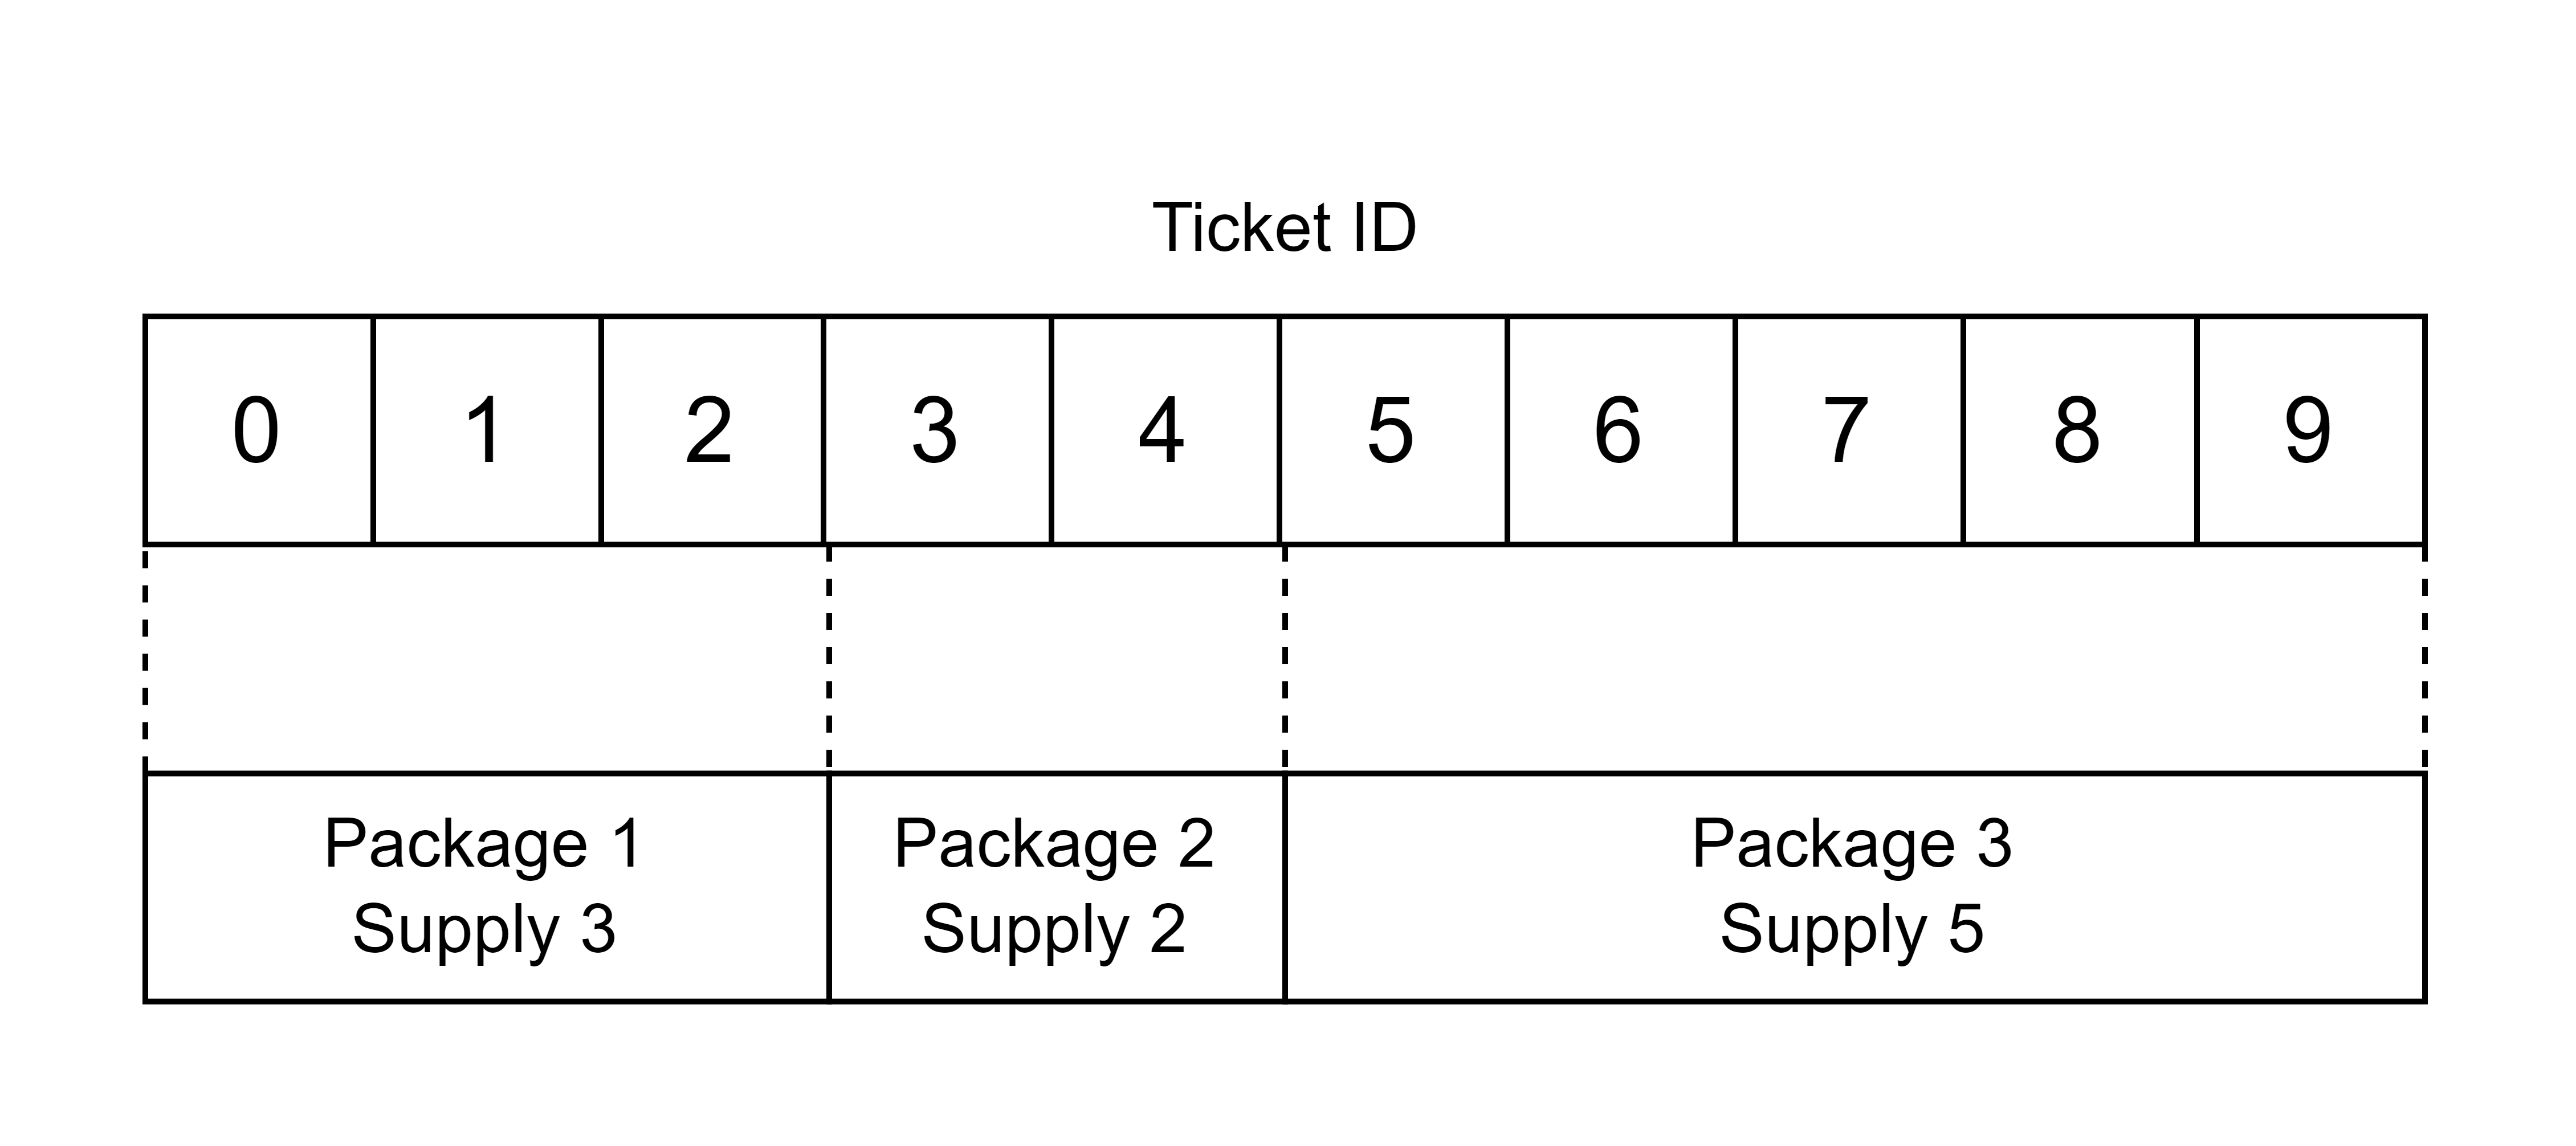
\includegraphics[width=\textwidth*2/3]{Package logic.png}
	\centering
	\caption{Package logic}
	\label{fig:package_logic}
\end{figure}

This way, whenever we need to get a ticket for a certain package, we can go
through the packages and see which one the ID is in. One only limitation with
this is if the event is already open (users can buy tickets), the only thing we
can allow the organizer to do is to add packages, neither remove or change
their order, because that would change the package associated to the tickets,
which would be a problem for the users that already bought them.

Now we just have to make sure the information obtained with the
\textit{tokenURI} method corresponds to the ticket, according to its package.
For this we will have a different metadata file for each package, with the
necessary information about the tickets. The \textit{individualNfts} boolean in
the \textit{PackageConfig} struct is there to indicate if the organizer wants
each ticket on the package to have its own metadata, or if they can share it.

According to this, the \textit{tokenURI} will return an URI like
'baseURI/packageId/ticketId' for a package with individual NFTs, and
'baseURI/packageId' for a package with shared metadata. Like this, when we
store the metadata on the IPFS, we store the metadata for each ticket inside a
folder of the packages with individual NFTs, and only a metadata file for each
package without individual NFTs.

\subsection{Metadata Storage}
\label{subsec:metadata_storage}

To store the NFTs metadata files, we'll be using the
\href{https://ipfs.tech/}{InterPlanetary File System (IPFS)} for storing the
NFTs metadata. The IPFS is a decentralized storage system where the data is
stored in a distributed network of nodes (decentralized), making it very secure
and reliable. This is a great solution for storing the metadata of the NFTs
because it's very cheap and easy to use, and it's a common practice in the
blockchain ecosystem.

Other options would be to store the data on some kind of server, but that would
be more expensive to maintain, and since we are dealing with NFTs, it's good
practice to store the data in a decentralized manner, to avoid any kind of
alteration on its contents, if the tickets possibly become valuable
collectibles.

This kind of issue was something that has happened before, where people bought
NFTs with the idea of them being somewhat valuable, but then the owner changed
the contents of the metadata, executing what was called of a \textit{rug pull},
which is a scam that made the NFTs worthless, keeping the money for himself.

To store the data on the IPFS, we will be using the
\href{https://www.pinata.cloud/}{Pinata} service, which does the heavy lifting
for interacting with the storage itself. To accomplish this, we just need to
arrange the files according to the ticket packages, like mentioned before in
the Section \ref{subsec:ticket_packages}, and then upload them to the IPFS,
getting the link to the metadata, which we'll then store on the contract as the
base URI. The files would be stored like the Figure \ref{fig:metadata_storage}
shows, being the packages 1 and 3 with shared metadata, and the package 2 with
individual NFTs.

\begin{figure}[H]
	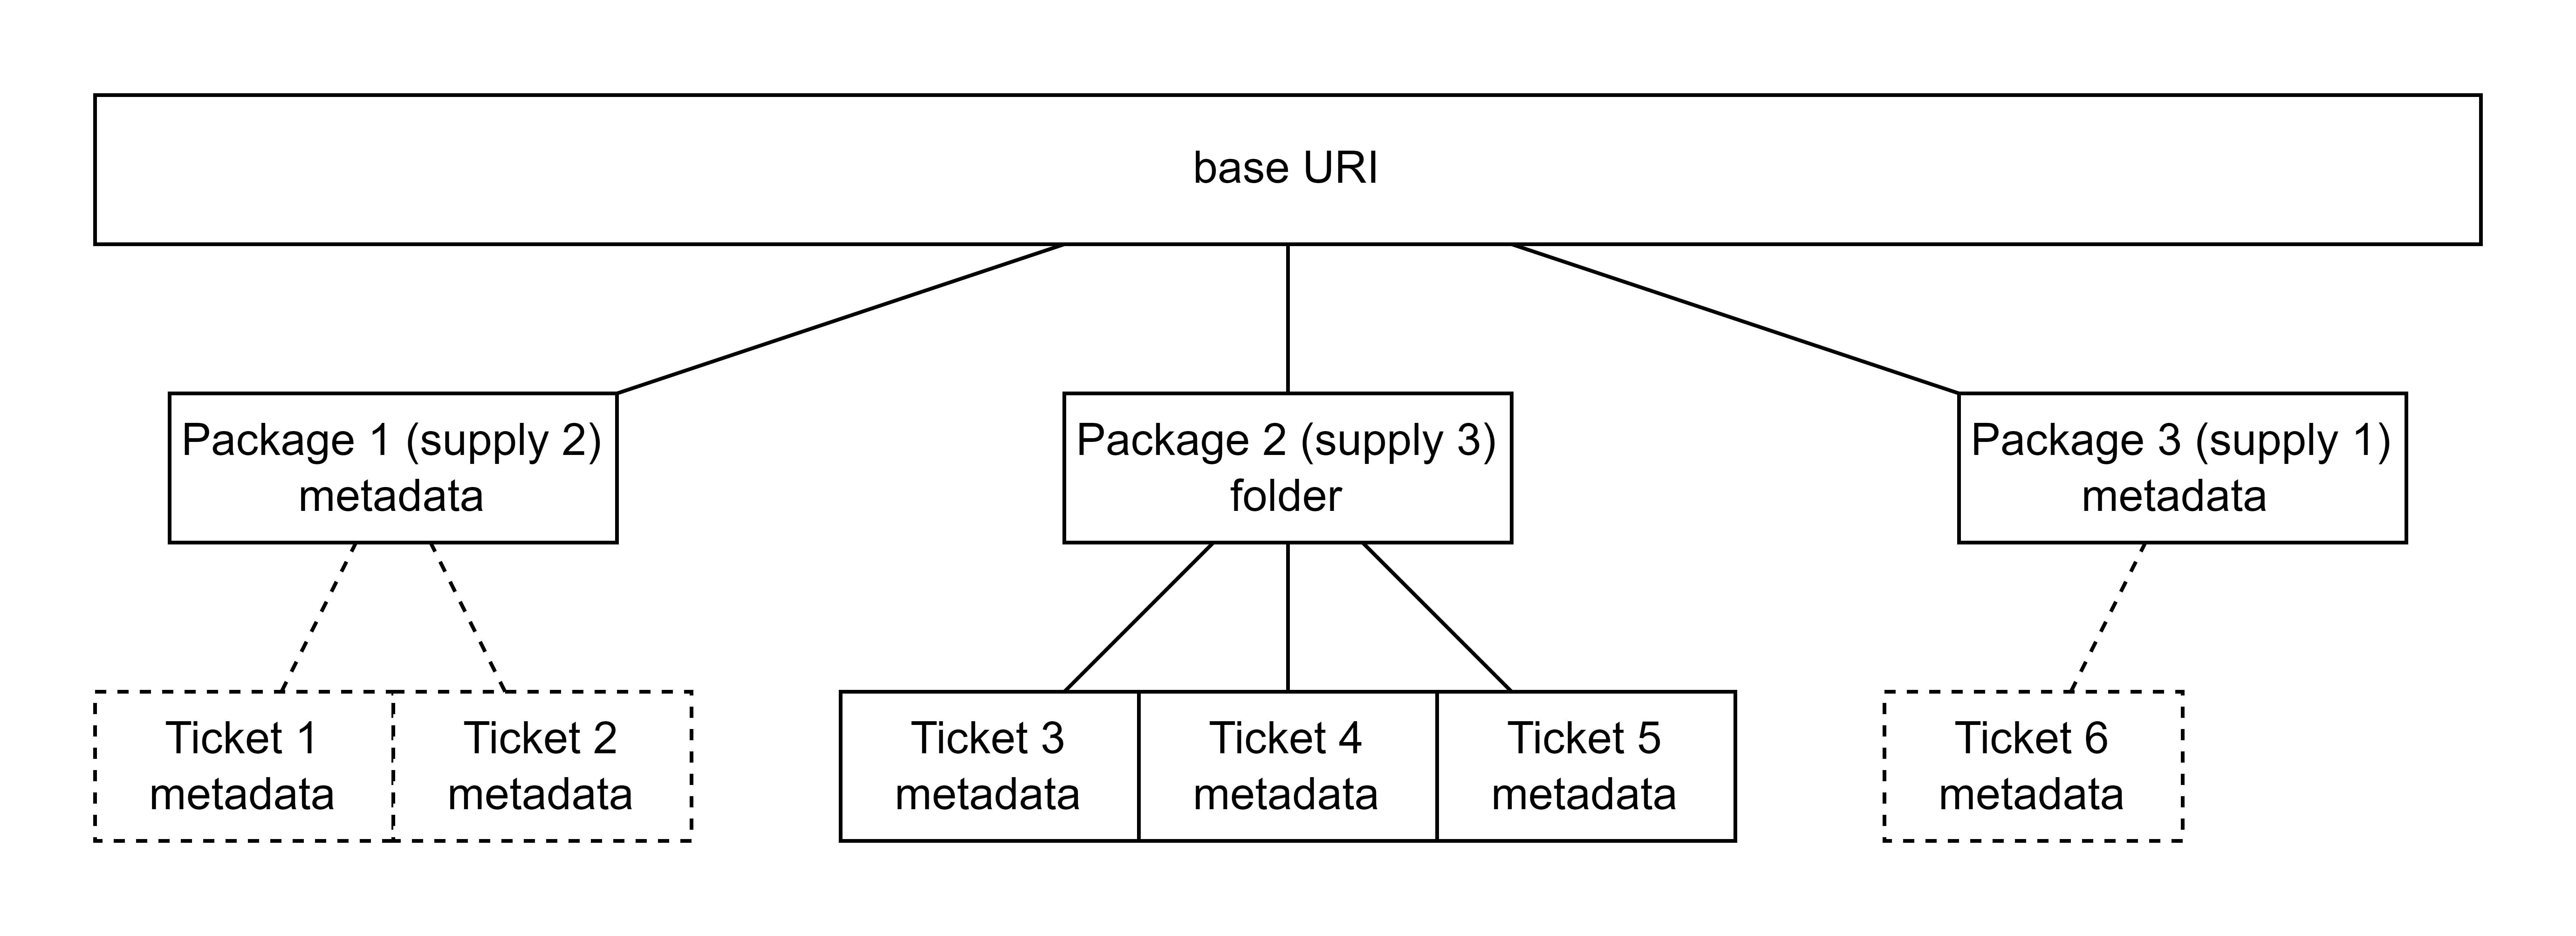
\includegraphics[width=\textwidth]{Metadata storage.png}
	\centering
	\caption{Metadata storage}
	\label{fig:metadata_storage}
\end{figure}

\subsection{System Fees}
\label{subsec:system_fees}

One of the most important aspects of a system like this is the business model
we have to take into account. Since this is a service we want to deploy for
event organizers, we need to make this sustainable and profitable. This kind of
service aims to do some heavy lifting, with its own features, so we could set a
fee lower than the usual on the traditional marketplaces and ticket selling
platforms, since the organizers need to pay for each service.

These low fees are possible because with the system being deployed on the
blockchain, it stays there while the network is running, so the only extra cost
are the network fees when interacting with the event. For the users, each
interaction is paid by them, so when a user buys a ticket, the only thing to
take into account are the network fees, which depending on the network, can be
super low.

The other kind of fee the organizer needs to look out for is for the validators
to validate the tickets, which is a necessary operation to avoid people from
exploiting the system. These fees are paid by the validators, which the
organizer essentially manages, so we need to take this into account when
setting the system fee, to make it sustainable for the organizer to use our
system.

We'll set a fee on the main smart contract, where will be stored in the event
when registering it, so that if we decide to change it, the previous events
aren't affected. This is also because we want to abstract the user of any extra
fee, so the price the organizer sets, is the price the user pays, and the
system fee is taken from the tickets price. In case an event gets cancelled, or
a user decides to get a refund, the ticket fee is returned to the user
(proportional to the refund), making the system less profit, but guarantees the
users of a fair process. With this, we need to restrict the system to only
withdraw any profit after the event is over. Since this is rather an uncommon
case, the less profit that the system makes compensates for the trust that the
users and organizers will have on it.

\pagebreak
\chapter{Results}

\section{Limitations}

\section{Future Work}

\pagebreak

\chapter{Conclusions}
\label{ch:conclusions}

\section{Limitations}
 [network fees]
 [finality]
 [connection to wallet can be unstable depending on the wallet]
 [users can still gift others in exchange for money, but we have to let users know they should only operate within the system]

\section{Future Work}

 [marketplace (resell)]
 [organizer dashboard]
 [mention how wei can be translated to any currency later]

\printbibliography[heading=bibintoc]

% \nocite{*}
% \bibliographystyle{plain}
% \bibliography{references}
% \appendix
% \chapter{Appendix}

\end{document}
